    
%% bare_conf.tex
%% V1.3
%% 2007/01/11
%% by Michael Shell
%% See:
%% http://www.michaelshell.org/
%% for current contact information.
%%
%% This is a skeleton file demonstrating the use of IEEEtran.cls
%% (requires IEEEtran.cls version 1.7 or later) with an IEEE conference paper.
%%
%% Support sites:
%% http://www.michaelshell.org/tex/ieeetran/
%% http://www.ctan.org/tex-archive/macros/latex/contrib/IEEEtran/
%% and
%% http://www.ieee.org/

%%*************************************************************************
%% Legal Notice:
%% This code is offered as-is without any warranty either expressed or
%% implied; without even the implied warranty of MERCHANTABILITY or
%% FITNESS FOR A PARTICULAR PURPOSE! 
%% User assumes all risk.
%% In no event shall IEEE or any contributor to this code be liable for
%% any damages or losses, including, but not limited to, incidental,
%% consequential, or any other damages, resulting from the use or misuse
%% of any information contained here.
%%
%% All comments are the opinions of their respective authors and are not
%% necessarily endorsed by the IEEE.
%%
%% This work is distributed under the LaTeX Project Public License (LPPL)
%% ( http://www.latex-project.org/ ) version 1.3, and may be freely used,
%% distributed and modified. A copy of the LPPL, version 1.3, is included
%% in the base LaTeX documentation of all distributions of LaTeX released
%% 2003/12/01 or later.
%% Retain all contribution notices and credits.
%% ** Modified files should be clearly indicated as such, including  **
%% ** renaming them and changing author support contact information. **
%%
%% File list of work: IEEEtran.cls, IEEEtran_HOWTO.pdf, bare_adv.tex,
%%                    bare_conf.tex, bare_jrnl.tex, bare_jrnl_compsoc.tex
%%*************************************************************************

% *** Authors should verify (and, if needed, correct) their LaTeX system  ***
% *** with the testflow diagnostic prior to trusting their LaTeX platform ***
% *** with production work. IEEE's font choices can trigger bugs that do  ***
% *** not appear when using other class files.                            ***
% The testflow support page is at:
% http://www.michaelshell.org/tex/testflow/



% Note that the a4paper option is mainly intended so that authors in
% countries using A4 can easily print to A4 and see how their papers will
% look in print - the typesetting of the document will not typically be
% affected with changes in paper size (but the bottom and side margins will).
% Use the testflow package mentioned above to verify correct handling of
% both paper sizes by the user's LaTeX system.
%
% Also note that the "draftcls" or "draftclsnofoot", not "draft", option
% should be used if it is desired that the figures are to be displayed in
% draft mode.
%
\documentclass[10pt, conference, compsocconf]{IEEEtran}
% Add the compsocconf option for Computer Society conferences.
%
% If IEEEtran.cls has not been installed into the LaTeX system files,
% manually specify the path to it like:
% \documentclass[conference]{../sty/IEEEtran}





% Some very useful LaTeX packages include:
% (uncomment the ones you want to load)


% *** MISC UTILITY PACKAGES ***
%
%\usepackage{ifpdf}
% Heiko Oberdiek's ifpdf.sty is very useful if you need conditional
% compilation based on whether the output is pdf or dvi.
% usage:
% \ifpdf
%   % pdf code
% \else
%   % dvi code
% \fi
% The latest version of ifpdf.sty can be obtained from:
% http://www.ctan.org/tex-archive/macros/latex/contrib/oberdiek/
% Also, note that IEEEtran.cls V1.7 and later provides a builtin
% \ifCLASSINFOpdf conditional that works the same way.
% When switching from latex to pdflatex and vice-versa, the compiler may
% have to be run twice to clear warning/error messages.






% *** CITATION PACKAGES ***
%
%\usepackage{cite}
% cite.sty was written by Donald Arseneau
% V1.6 and later of IEEEtran pre-defines the format of the cite.sty package
% \cite{} output to follow that of IEEE. Loading the cite package will
% result in citation numbers being automatically sorted and properly
% "compressed/ranged". e.g., [1], [9], [2], [7], [5], [6] without using
% cite.sty will become [1], [2], [5]--[7], [9] using cite.sty. cite.sty's
% \cite will automatically add leading space, if needed. Use cite.sty's
% noadjust option (cite.sty V3.8 and later) if you want to turn this off.
% cite.sty is already installed on most LaTeX systems. Be sure and use
% version 4.0 (2003-05-27) and later if using hyperref.sty. cite.sty does
% not currently provide for hyperlinked citations.
% The latest version can be obtained at:
% http://www.ctan.org/tex-archive/macros/latex/contrib/cite/
% The documentation is contained in the cite.sty file itself.






% *** GRAPHICS RELATED PACKAGES ***
%
\ifCLASSINFOpdf
  \usepackage[pdftex]{graphicx}
  % declare the path(s) where your graphic files are
  % \graphicspath{{../pdf/}{../jpeg/}}
  % and their extensions so you won't have to specify these with
  % every instance of \inputgraphics
  % \DeclareGraphicsExtensions{.pdf,.jpeg,.png}
\else
  % or other class option (dvipsone, dvipdf, if not using dvips). graphicx
  % will default to the driver specified in the system graphics.cfg if no
  % driver is specified.
   \usepackage[dvips]{graphicx}
  % declare the path(s) where your graphic files are
  % \graphicspath{{../eps/}}
  % and their extensions so you won't have to specify these with
  % every instance of \inputgraphics
  % \DeclareGraphicsExtensions{.eps}
\fi
% graphicx was written by David Carlisle and Sebastian Rahtz. It is
% required if you want graphics, photos, etc. graphicx.sty is already
% installed on most LaTeX systems. The latest version and documentation can
% be obtained at: 
% http://www.ctan.org/tex-archive/macros/latex/required/graphics/
% Another good source of documentation is "Using Imported Graphics in
% LaTeX2e" by Keith Reckdahl which can be found as epslatex.ps or
% epslatex.pdf at: http://www.ctan.org/tex-archive/info/
%
% latex, and pdflatex in dvi mode, support graphics in encapsulated
% postscript (.eps) format. pdflatex in pdf mode supports graphics
% in .pdf, .jpeg, .png and .mps (metapost) formats. Users should ensure
% that all non-photo figures use a vector format (.eps, .pdf, .mps) and
% not a bitmapped formats (.jpeg, .png). IEEE frowns on bitmapped formats
% which can result in "jaggedy"/blurry rendering of lines and letters as
% well as large increases in file sizes.
%
% You can find documentation about the pdfTeX application at:
% http://www.tug.org/applications/pdftex





% *** MATH PACKAGES ***
%
%\usepackage[cmex10]{amsmath}
% A popular package from the American Mathematical Society that provides
% many useful and powerful commands for dealing with mathematics. If using
% it, be sure to load this package with the cmex10 option to ensure that
% only type 1 fonts will utilized at all point sizes. Without this option,
% it is possible that some math symbols, particularly those within
% footnotes, will be rendered in bitmap form which will result in a
% document that can not be IEEE Xplore compliant!
%
% Also, note that the amsmath package sets \interdisplaylinepenalty to 10000
% thus preventing page breaks from occurring within multiline equations. Use:
%\interdisplaylinepenalty=2500
% after loading amsmath to restore such page breaks as IEEEtran.cls normally
% does. amsmath.sty is already installed on most LaTeX systems. The latest
% version and documentation can be obtained at:
% http://www.ctan.org/tex-archive/macros/latex/required/amslatex/math/





% *** SPECIALIZED LIST PACKAGES ***
%
%\usepackage{algorithmic}
% algorithmic.sty was written by Peter Williams and Rogerio Brito.
% This package provides an algorithmic environment fo describing algorithms.
% You can use the algorithmic environment in-text or within a figure
% environment to provide for a floating algorithm. Do NOT use the algorithm
% floating environment provided by algorithm.sty (by the same authors) or
% algorithm2e.sty (by Christophe Fiorio) as IEEE does not use dedicated
% algorithm float types and packages that provide these will not provide
% correct IEEE style captions. The latest version and documentation of
% algorithmic.sty can be obtained at:
% http://www.ctan.org/tex-archive/macros/latex/contrib/algorithms/
% There is also a support site at:
% http://algorithms.berlios.de/index.html
% Also of interest may be the (relatively newer and more customizable)
% algorithmicx.sty package by Szasz Janos:
% http://www.ctan.org/tex-archive/macros/latex/contrib/algorithmicx/




% *** ALIGNMENT PACKAGES ***
%
%\usepackage{array}
% Frank Mittelbach's and David Carlisle's array.sty patches and improves
% the standard LaTeX2e array and tabular environments to provide better
% appearance and additional user controls. As the default LaTeX2e table
% generation code is lacking to the point of almost being broken with
% respect to the quality of the end results, all users are strongly
% advised to use an enhanced (at the very least that provided by array.sty)
% set of table tools. array.sty is already installed on most systems. The
% latest version and documentation can be obtained at:
% http://www.ctan.org/tex-archive/macros/latex/required/tools/


%\usepackage{mdwmath}
%\usepackage{mdwtab}
% Also highly recommended is Mark Wooding's extremely powerful MDW tools,
% especially mdwmath.sty and mdwtab.sty which are used to format equations
% and tables, respectively. The MDWtools set is already installed on most
% LaTeX systems. The lastest version and documentation is available at:
% http://www.ctan.org/tex-archive/macros/latex/contrib/mdwtools/


% IEEEtran contains the IEEEeqnarray family of commands that can be used to
% generate multiline equations as well as matrices, tables, etc., of high
% quality.


%\usepackage{eqparbox}
% Also of notable interest is Scott Pakin's eqparbox package for creating
% (automatically sized) equal width boxes - aka "natural width parboxes".
% Available at:
% http://www.ctan.org/tex-archive/macros/latex/contrib/eqparbox/





% *** SUBFIGURE PACKAGES ***
%\usepackage[tight,footnotesize]{subfigure}
% subfigure.sty was written by Steven Douglas Cochran. This package makes it
% easy to put subfigures in your figures. e.g., "Figure 1a and 1b". For IEEE
% work, it is a good idea to load it with the tight package option to reduce
% the amount of white space around the subfigures. subfigure.sty is already
% installed on most LaTeX systems. The latest version and documentation can
% be obtained at:
% http://www.ctan.org/tex-archive/obsolete/macros/latex/contrib/subfigure/
% subfigure.sty has been superceeded by subfig.sty.



%\usepackage[caption=false]{caption}
%\usepackage[font=footnotesize]{subfig}
% subfig.sty, also written by Steven Douglas Cochran, is the modern
% replacement for subfigure.sty. However, subfig.sty requires and
% automatically loads Axel Sommerfeldt's caption.sty which will override
% IEEEtran.cls handling of captions and this will result in nonIEEE style
% figure/table captions. To prevent this problem, be sure and preload
% caption.sty with its "caption=false" package option. This is will preserve
% IEEEtran.cls handing of captions. Version 1.3 (2005/06/28) and later 
% (recommended due to many improvements over 1.2) of subfig.sty supports
% the caption=false option directly:
%\usepackage[caption=false,font=footnotesize]{subfig}
%
% The latest version and documentation can be obtained at:
% http://www.ctan.org/tex-archive/macros/latex/contrib/subfig/
% The latest version and documentation of caption.sty can be obtained at:
% http://www.ctan.org/tex-archive/macros/latex/contrib/caption/




% *** FLOAT PACKAGES ***
%
%\usepackage{fixltx2e}
% fixltx2e, the successor to the earlier fix2col.sty, was written by
% Frank Mittelbach and David Carlisle. This package corrects a few problems
% in the LaTeX2e kernel, the most notable of which is that in current
% LaTeX2e releases, the ordering of single and double column floats is not
% guaranteed to be preserved. Thus, an unpatched LaTeX2e can allow a
% single column figure to be placed prior to an earlier double column
% figure. The latest version and documentation can be found at:
% http://www.ctan.org/tex-archive/macros/latex/base/



%\usepackage{stfloats}
% stfloats.sty was written by Sigitas Tolusis. This package gives LaTeX2e
% the ability to do double column floats at the bottom of the page as well
% as the top. (e.g., "\begin{figure*}[!b]" is not normally possible in
% LaTeX2e). It also provides a command:
%\fnbelowfloat
% to enable the placement of footnotes below bottom floats (the standard
% LaTeX2e kernel puts them above bottom floats). This is an invasive package
% which rewrites many portions of the LaTeX2e float routines. It may not work
% with other packages that modify the LaTeX2e float routines. The latest
% version and documentation can be obtained at:
% http://www.ctan.org/tex-archive/macros/latex/contrib/sttools/
% Documentation is contained in the stfloats.sty comments as well as in the
% presfull.pdf file. Do not use the stfloats baselinefloat ability as IEEE
% does not allow \baselineskip to stretch. Authors submitting work to the
% IEEE should note that IEEE rarely uses double column equations and
% that authors should try to avoid such use. Do not be tempted to use the
% cuted.sty or midfloat.sty packages (also by Sigitas Tolusis) as IEEE does
% not format its papers in such ways.





% *** PDF, URL AND HYPERLINK PACKAGES ***
%
\usepackage{url}
% url.sty was written by Donald Arseneau. It provides better support for
% handling and breaking URLs. url.sty is already installed on most LaTeX
% systems. The latest version can be obtained at:
% http://www.ctan.org/tex-archive/macros/latex/contrib/misc/
% Read the url.sty source comments for usage information. Basically,
% \url{my_url_here}.

% For colouring and commenting during draft stages
\usepackage{xcolor}



% *** Do not adjust lengths that control margins, column widths, etc. ***
% *** Do not use packages that alter fonts (such as pslatex).         ***
% There should be no need to do such things with IEEEtran.cls V1.6 and later.
% (Unless specifically asked to do so by the journal or conference you plan
% to submit to, of course. )


% correct bad hyphenation here
\hyphenation{op-tical net-works semi-conduc-tor}

\newtheorem{definition}{Definition}
\newtheorem{result}{Result}
\newtheorem{remark}{Remark}
\usepackage{amssymb}
\usepackage{amsmath}
\usepackage{algorithm}
\usepackage{algorithmic}
\usepackage{tikz-network}
\usepackage{subfigure}
\newcommand{\dd}{\mathop{}\!\mathrm{d}}
\DeclareMathOperator{\vect}{vec}

\begin{document}
%
% paper title
% can use linebreaks \\ within to get better formatting as desired
\title{Serums: Securing Medical Data in Smart Patient-Centric Healthcare Systems}


% author names and affiliations
% use a multiple column layout for up to two different
% affiliations

\author{\IEEEauthorblockN{Vladimir Janjic, Juliana Bowles, Andreas Francois Vermeulen, Agastya Silvina}
\IEEEauthorblockA{\textit{School of Computer Science, University of St Andrews} \\
St Andrews, United  Kingdom \\
\url{{vj32,jkfb,afv}@st-andrews.ac.uk}}
\and
\IEEEauthorblockN{Marios Belk, Andreas Pitsillides}
\IEEEauthorblockA{\textit{Department of Computer Science, University of Cyprus} \\
Nicosia, Cyprus \\
\url{{belk, andreas.pitsillides}@cs.ucy.ac.cy}}
\and
\IEEEauthorblockN{Mohit Kumar, Michael Rossbory}
\IEEEauthorblockA{\textit{Data Analysis Systems} \\
\textit{Software Competence Center Hagenberg}\\
Hagenberg, Austria \\
\url{{mohit.kumar,michael.rossbory}@scch.at}}
\and
\IEEEauthorblockN{4\textsuperscript{th} Given Name Surname}
\IEEEauthorblockA{\textit{dept. name of organization (of Aff.)} \\
\textit{name of organization (of Aff.)}\\
City, Country \\
email address}
\and
\IEEEauthorblockN{5\textsuperscript{th} Given Name Surname}
\IEEEauthorblockA{\textit{dept. name of organization (of Aff.)} \\
\textit{name of organization (of Aff.)}\\
City, Country \\
email address}
\and
\IEEEauthorblockN{6\textsuperscript{th} Given Name Surname}
\IEEEauthorblockA{\textit{dept. name of organization (of Aff.)} \\
\textit{name of organization (of Aff.)}\\
City, Country \\
email address}
}

% conference papers do not typically use \thanks and this command
% is locked out in conference mode. If really needed, such as for
% the acknowledgment of grants, issue a \IEEEoverridecommandlockouts
% after \documentclass

% for over three affiliations, or if they all won't fit within the width
% of the page, use this alternative format:
% 
%\author{\IEEEauthorblockN{Michael Shell\IEEEauthorrefmark{1},
%Homer Simpson\IEEEauthorrefmark{2},
%James Kirk\IEEEauthorrefmark{3}, 
%Montgomery Scott\IEEEauthorrefmark{3} and
%Eldon Tyrell\IEEEauthorrefmark{4}}
%\IEEEauthorblockA{\IEEEauthorrefmark{1}School of Electrical and Computer Engineering\\
%Georgia Institute of Technology,
%Atlanta, Georgia 30332--0250\\ Email: see http://www.michaelshell.org/contact.html}
%\IEEEauthorblockA{\IEEEauthorrefmark{2}Twentieth Century Fox, Springfield, USA\\
%Email: homer@thesimpsons.com}
%\IEEEauthorblockA{\IEEEauthorrefmark{3}Starfleet Academy, San Francisco, California 96678-2391\\
%Telephone: (800) 555--1212, Fax: (888) 555--1212}
%\IEEEauthorblockA{\IEEEauthorrefmark{4}Tyrell Inc., 123 Replicant Street, Los Angeles, California 90210--4321}}




% use for special paper notices
%\IEEEspecialpapernotice{(Invited Paper)}




% make the title area
\maketitle


\begin{abstract}
Paper due: 27 July 2019

\end{abstract}

\begin{IEEEkeywords}
component; formatting; style; styling;

\end{IEEEkeywords}

\IEEEpeerreviewmaketitle

% Call for papers
% http://cci.drexel.edu/bigdata/bigdata2019/SpecialSession.html#SpecialSession4
% submission guidelines
% http://cci.drexel.edu/bigdata/bigdata2019/CallPapers.html
% NOTES
% 10 page IEEE 2-column format
% single blind reviews

\section{Introduction}
\noindent
The healthcare systems of the future will be highly decentralised, integrating home-, work- and environment-based monitoring into the hospital diagnostic systems, thus reducing costs and travel-associated risks while allowing patients to get better medical treatment (Figure~\ref{fig:dataExch}). As a consequence, medical data will need to be collected from a variety of sources and exchanged in a variety of ways, including over public networks that cannot be implicitly trusted. At the same time, we have more and more strict regulations about ownership and access rights for the patient data. Trans-national standards for data protection, such as GDPR~\cite{gdpr}, will need to be combined with local regulations, giving very strict rules about who is allowed to access what data. Complying with these rules while, at the same time, facilitating data exchange and analytics in much more distributed way will be the main challenge for the modern healtcare systems.  

\begin{figure}[h!]
    \centering
    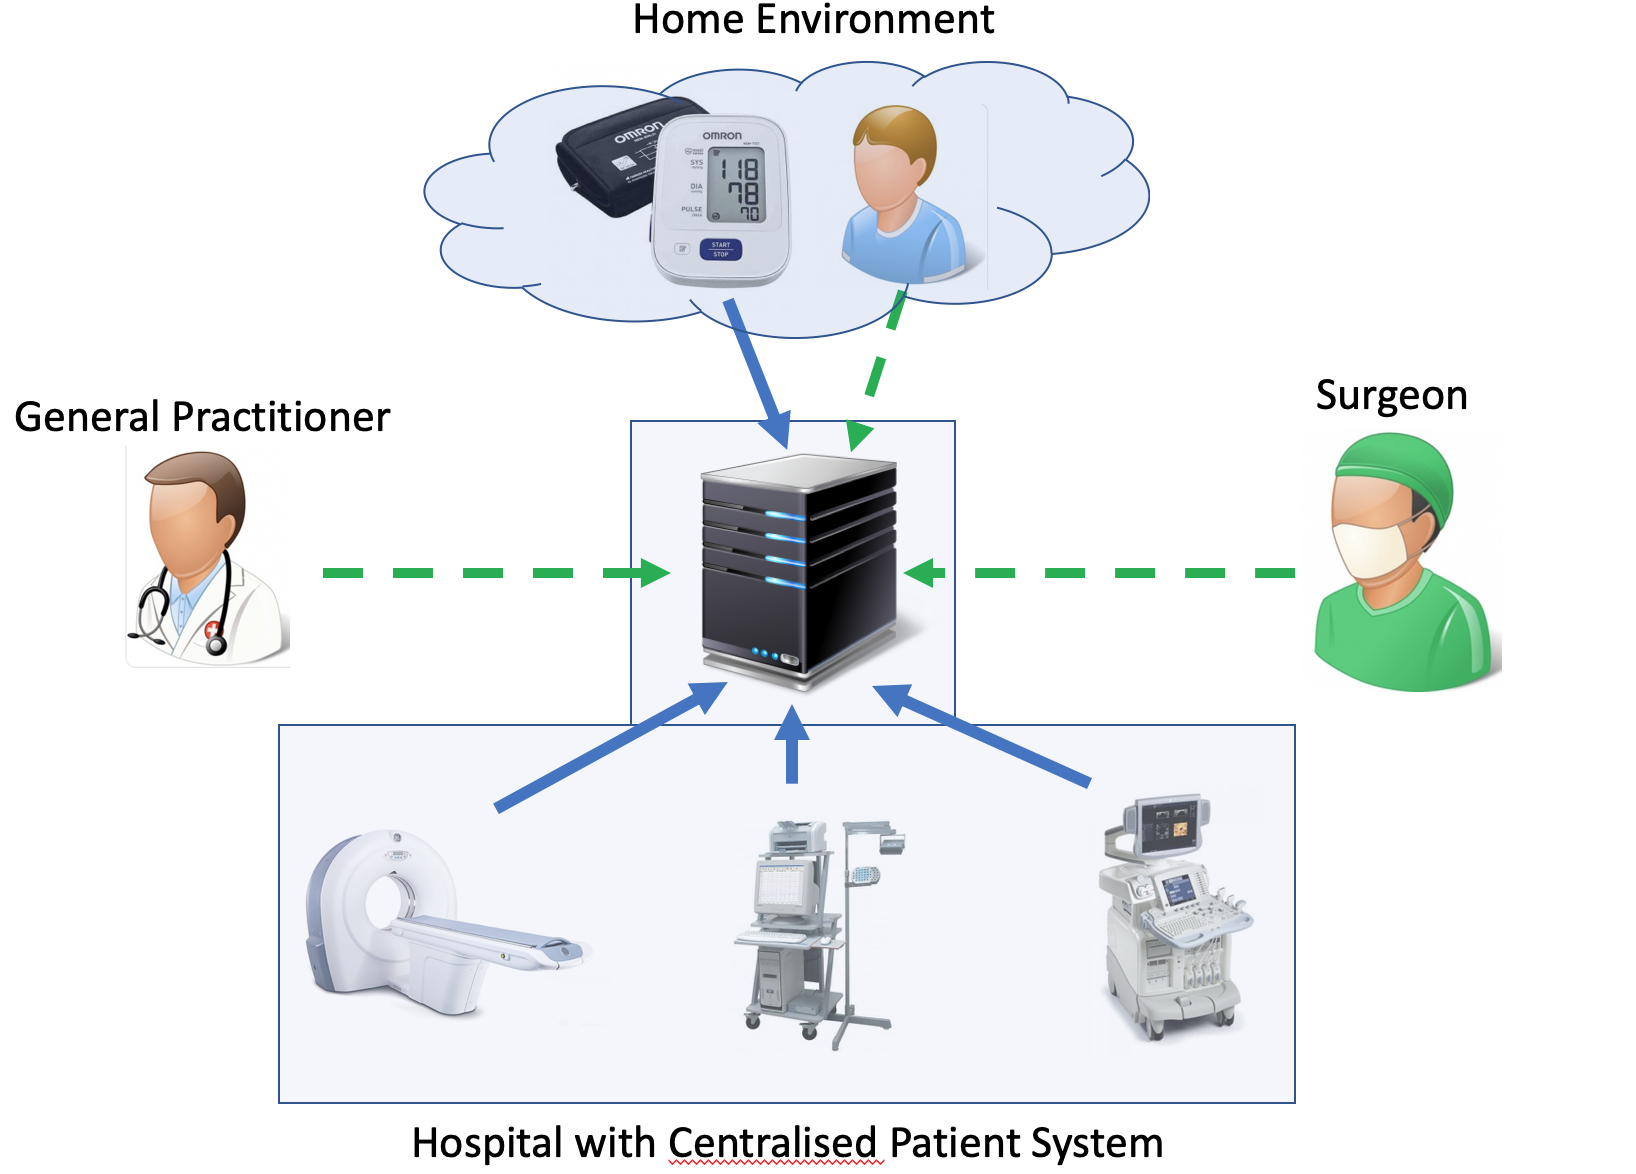
\includegraphics[scale=0.3]{images/DataExchange.png}
    \caption{Data Exhcange in Modern Healthcare Systems}
    \label{fig:dataExch}
\end{figure}



\subsection*{Notes}

Here are the items from the call for Healthcare Data and some comments/notes:
\begin{enumerate}
\item 
\emph{Health data collection and analysis:}
We have a lot of basis on this, we are clearly in both collection analytics.

\item 
\emph{Problems in health data processing:}
We have some data processing aspects, so this is also strong for us.

\item 
\emph{Protection and security of personal health data:}
We have this conceptually, and also concrete connections to GDPR.

\item 
\emph{Electronic health records and standards:}
Exactly what we're doing for the first parts, standards not so clear?
\end{enumerate}





\section{Serums Technologies}
\subsection{Smart Patient Records}

% Sopra-Steria, Scotland, UK

\noindent
Good organisation of patient data is essential to the smooth and correct operation of any health system. 
%This includes the traditional requirements of
%ease of accessibility and precise structure of the records.
Furthermore, new legislation for privacy and ownership of the data (such as GDPR) together with a highly-decentralised organisation of modern health providers impose additional requirements for health data. Ideally, patient data should be owned by the patient, and only they have full access to their data. Other system users, such as specialists, general practitioners and insurers, are expected to have access to parts of the data relevant to the services they provide (e.g.~diagnostics, treatment, insurance etc.). In addition to access restrictions, the distributed nature of health systems means that we cannot assume that data is stored in one central location. Secure communication of data across untrusted networks might be required at any point the patient record is accessed. To develop a generic infrastructure for safe and secure communication of distributed medical data, it is highly desirable for the patient data (including pointers to any data that resides on remote systems) to be stored in a precise and machine-readable format.

In the \emph{SERUMS} technology tool-chain, the \emph{Smart Patient Record} represents a central information source for information about patients registered in Europe. These records aggregate a complete patient medical history across approved healthcare providers. The information in a single record includes both relatively static information (such as name, age, address, type of insurance, allergies) and highly dynamic information (such as undergoing treatments, results of scans and hospital admissions). For each healthcare institution, smart patient records will reside in a \emph{Smart Healthcare Data Lake}. The \emph{Smart Patient Record Format} represents metadata that describes the data in the records. 
%One of the main goals of the \emph{SERUMS} project is to 
We propose a \emph{universal} format for patient records that can be used for describing different use cases within SERUMS and is applicable to future healthcare systems.

Our universal format is based on the concept of \emph{data vault}~\cite{Inmon2015}, which consists of \emph{hubs} (unique business keys), \emph{links} (that represent associations between hubs) and \emph{satellites} (where attributes of the hubs and links are stored). 
%\subsubsection{Data Vault}
%
%A \emph{data vault} defines guidelines on how to organise the tables and relationships within a database system,  
%As such, it can work on top of any database system such as PostgreSQL, a distributed file system such as Hadoop, or even a NoSQL database such as MongoDB. 
%and has  been  designed  to  take  in  data  from  disparate sources and systems and centralise the data in a non-destructive manner. End users do not interact directly with the raw data in the database, but with a layer of cleansed data which is produced on top in the form of a data warehouse. The data vault model is comprised of  \emph{hubs} (that  contain  a  list  of  unique  business  keys  with  low  propensity  to change), \emph{links} (that represent associations or transactions between hubs) and \emph{satellites} (where temporal and descriptive attributes of the hubs and links are stored).
%
%We have chosen to use the data vault as the format to represent patient records because it supports a structure that stores data in a history preserving methodology. 
%using Disciplined Agile Deliveries (DAD) {\color{red}[VJ: Citation?]}. 
%The long-term functionality of the data vault can evolve as requirements change. %The natural hub-link-satellite structure empowers the 
%Furthermore, it makes it possible to use an insert-only data loading methodology to merge parallel data sources together and introduce the requirements rapidly as information becomes available from the various health care providers.
%
%VJ : This was all pretty much said above
%AV : Accepted and now marked for removal from document
%The \emph{data vault} format supports both static and dynamic patient data and can cover the complete data cycle of the patients' interaction with the system. For example, when a patient is admitted to hospital, their current status may change rapidly (and their diagnosis). The data vault enables to record how the information becomes available from the systems. Therefore, on admission to the hospital, a patient is registered with a record that supports both static (and immutable) data and dynamic data that covers the ever-changing parts of their interactions with the health systems, making the history of the interactions immutable and relevant at all times during the patients visit.
%%
%
%
%\subsubsection{T-P-O-L-E Data Vault as Universal Smart Patient Record Format} \label{sec:tpole}
The general data vault has unlimited types of hubs, links and satellites to model real-world data. The SERUMS project has introduced a more limited type of hub, link and satellite classification \cite{Linstedt2012} to force a more generalised view of all data sources. This will support scaling \cite{Linstedt2016} of the data vault. We propose a \emph{Time-Person-Object-Location-Event (T-P-O-L-E)} data vault as a universal smart patient record format, such that:
%T-P-O-L-E data vault consists of the following hubs.

\begin{itemize}
    \item \emph{Time}: the dates and times of events are stored in Coordinated Universal Time.
    \item \emph{Person}: information  about  patients  is  stored  using  the  concept of "Golden Nominal".  This type of record is a single person record with a unique reference to that person.
    \item \emph{Object}: other referable entities that are stored, including organisations (hospital, bank, medicine suppliers etc.), physical objects (medicine, bank cards, vehicles, hospital beds), buildings etc.
    \item \emph{Location}: described by latitude, longitude and altitude \cite{Li2016a}.
    \item \emph{Event}: an abstraction of any event or action in the real-world, including scans, home visits by a doctor and treatments. 
\end{itemize}
The T-P-O-L-E data vault supports a future-proof design of the healthcare solution by enabling adding data at any point with full history capabilities. This model is the basis for the single-truth records data sharing and processing engine of the SERUMS project. The solution then uses advanced security to protect the information in a cross-country configuration respecting patient consent. This health record system will be able to support evolving coordinated services~\cite{Silow-Carroll2012} 

%\subsection{Smart Patient Records pt2}
\noindent
% VJ: We had all of this above, I think
% AV : Accepted - Suggest we remove the complete document from the bigger document.

%\paragraph{The Smart Patient Health Record (SPHR) is the combination of a patient's data, and the patient's control over access to their data. By gathering together all of the data into a single source, we allow the patient to have direct control over who can see what.}

%\paragraph{Our stated our choice for database format is Data Vault. This is a highly flexible format that will allow for continuous changes to what is stored in them, future-proofing the underlying design of the SPHR.}

%\begin{figure}
%    \centering
%    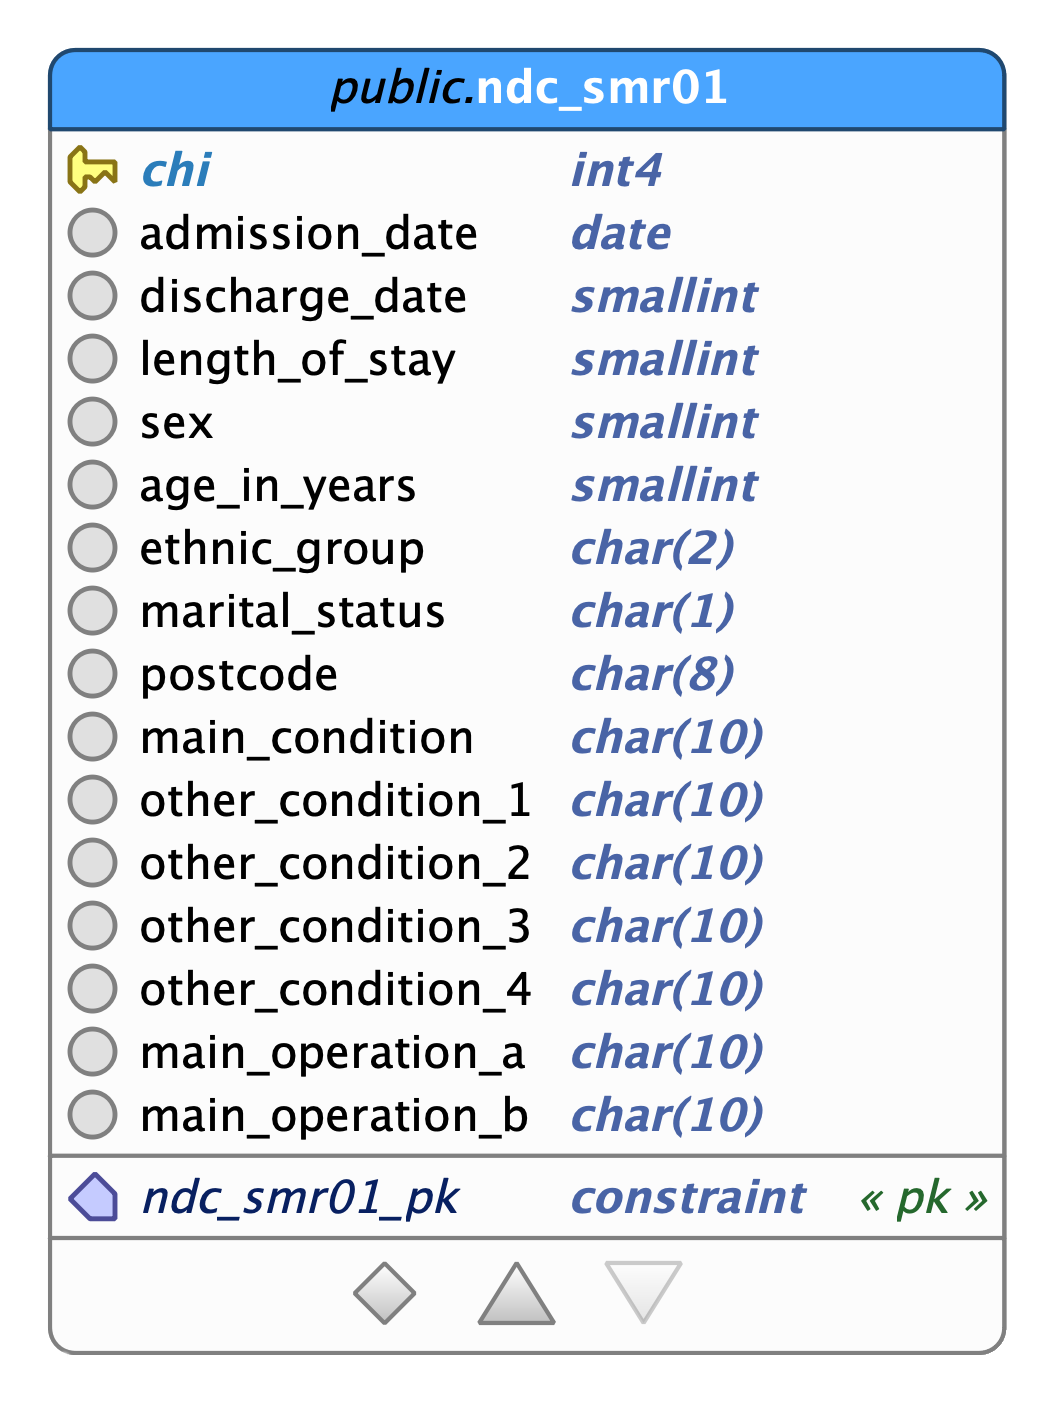
\includegraphics[width=45mm]{images/DataVault/smr01_source.png}
%    \caption{Example of source table}
%    \label{fig:smr01_source}
%\end{figure}


%\begin{figure}
 %   \centering
  %  \includegraphics[width=80mm]{images/DataVault/DataVault.pdf}
   % \caption{Example of source table abstracted into Data Vault}
    %\label{fig:dv_smr01}
%\end{figure}

%For example, Figure~\ref{fig:smr01_source} shows a part of the Edinburgh Cancer Gateway Centre use case, described in more detail in Section~\ref{sec:XX}. It contains information about one hospital visit of one patient. When abstracted into a data vault, the person hub would refer to patients, the time hub would refer to the dates and times of the hospital visits, and the object hub would contain the operations. The person hub contains the \emph{person demographic details} satellite, the time hub contains the \emph{admission date} satellite and the object hub contains the \emph{operations} and \emph{conditions} satellites (See Figure~\ref{fig:dv_smr01}).

\subsection{Data Fabrication}



\noindent
\label{sec:dfp}
IBM’s Data Fabrication Platform (DFP) is a web based central platform that provides a consistent and organisational-wide methodology (\emph{rule-guided fabrication}) for generating high-quality data for testing, development, and training. Fabrication of synthetic data consists of two stages - \emph{data modelling} and \emph{data generation}. Furthermore, data modelling comprises \emph{resources and structure definitions}, \emph{constraint rules definitions} and \emph{fabrication configuration definitions}. Input and output resources are standard relational databases (e.g., DB2, Oracle, PostgreSQL, SQLite), standard file formats (e.g., Flat file, XLS, CSV, XML, JSON) and streaming via MQTT protocol.

In rule guided fabrication, the database logic is extracted automatically and is augmented by application logic and testing logic modelled by the user. The application logic and the testing logic can be modelled using rules that the platform provides, but the users can also add new rules. Once the user requests the generation of a certain amount of data into a set of test databases, the platform internally ensures that the generated data satisfies the modelled rules as well as the internal databases consistency requirements. The platform can generate data from scratch, inflate existing databases, move existing data, and transform data from previously existing resources, such as old test databases or even production data. The platform provides a comprehensive and hybrid solution that can create a mixture of synthetic and real data according to user requirements.

\begin{figure}
    \centering
    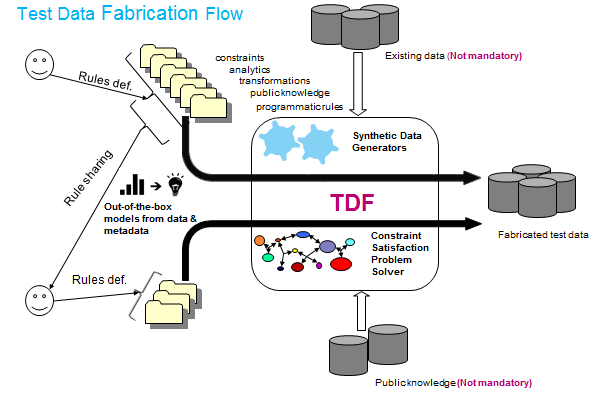
\includegraphics[width=0.45\textwidth]{images/DFPPlatformFlow.png}
    \caption{Flow of Generating Fabricated Data}
    \label{fig:dataFab}
\end{figure}

To overcome the shortcomings of existing data generation techniques, DFP generates data using a proprietary \emph{Constraint Satisfaction Problem (CPS)} solver (See Figure~\ref{fig:dataFab}). This methodology is generic and does not require access to real data, making it very safe to use in our setting. Data fabrication consists of the following steps.
\begin{enumerate}
\item The user defines a data project which contains the structure of the data, the constraint rules and the fabrication configuration. In order to construct a constraint satisfaction problem for the solver, the platform analyses the table metadata to get the desired properties (columns data types, referential integrity constraints etc.). 
\item The platform then selects a subset of the relevant rules and tables using the fabrication configuration, with possible addition of relevant parent tables and some default rules (e.g. PK and Unique Column). This information is used for the construction of a database table dependency graph. For each table in that graph, starting at root nodes, structural record dependencies are built recursively.
\item Based on the dependency graph, the fabrication pattern is computed where each target table record is assigned to one of the following fabrication modes: ‘New’, ‘Reuse’ or ‘Other’. Given the patterns, the graph and the rules, a CSP problem can be created. The problem consists of variables and rules, and a solution is an assignment of values to variables that satisfies the rules. 
\item Finally, the CSP problem is submitted to the solver, which produces a desired number of solutions to the problem and stores them in the appropriate places (e.g.~database, file or stream).
\end{enumerate} 



\subsection{Distributed Privacy-Preserving Data Analytics}\label{sec:dataanalysis}

\noindent
\label{sec:dataanalytics}
%Machine learning techniques are becoming increasingly important for many data-analytics models, and healthcare data analysis is no exception. 
\noindent
Machine learning methods such as deep neural networks have delivered remarkable results in data-analytics for a wide range of application domains, including healthcare. However, their training requires large data-sets which might be containing sensitive information that need to be be protected from \emph{model inversion} attack~\cite{Fredrikson:2015:MIA:2810103.2813677} and adversaries with access to model parameters and knowledge of the training procedure. This problem is addressed within the framework of differential privacy~\cite{Abadi:2016:DLD:2976749.2978318,Phan:2016:DPP:3015812.3016005}. Machine learning algorithms typically operate on data in the form of a matrix where e.g. rows correspond to features and columns correspond to samples. The particular problem in the context of matrix-valued data is to protect a machine learning algorithm, under differential privacy framework, from an adversary who seeks to gain an information about the data from an algorithm's output by perturbing the value in an element of the training data matrix. Despite the fact that random noise adding mechanism has been widely studied in privacy-preserving machine learning, there remains the challenge of studying privacy-utility trade-off for matrix-valued query functions. Our recent work~\cite{Kumar/IWCFS2019} has suggested a novel entropy based approach for resolving the privacy-utility trade-off for real-valued data matrices. The study in~\cite{Kumar/IWCFS2019}  mathematically derives the probability density function of noise that minimizes the expected noise magnitude together with satisfying sufficient conditions for $(\epsilon,\delta)-$differential privacy.

\subsubsection{An Optimal $(\epsilon,\delta)-$Differentially Private Noise for Real-Valued Matrices}
Consider a data-set consisting of $N$ number of samples with each sample having $p$ number of attributes represented by a matrix $\mathrm{Y} \in \mathbb{R}^{p \times N}$. A given machine learning algorithm, training a model using data matrix $\mathrm{Y}$, can be represented by a mapping, $\mathcal{A}: \mathbb{R}^{p \times N} \rightarrow \mathbf{M}$, where $\mathbf{M}$ is the model space.  
\begin{definition}[A Private Algorithm]\label{definition_private_algorithm}
Let $\mathcal{A}^+ : \mathbb{R}^{p \times N} \rightarrow Range(\mathcal{A}^+)$ be a mapping defined as
\begin{IEEEeqnarray}{rCl}
\mathcal{A}^+\left(\mathrm{Y}\right) & = & \mathcal{A}\left(\mathrm{Y} + \mathrm{V}\right),\;  \mathrm{V} \in \mathbb{R}^{p \times N}
\end{IEEEeqnarray}  
where $\mathrm{V}$ is a random noise matrix with $f_{\mathrm{v}_j^i}(v)$ being the probability density function of its $(j,i)-$th element $\mathrm{v}_j^i$; $\mathrm{v}_j^i$ and $\mathrm{v}_j^{i^{\prime}}$ are independent from each other for $i \neq i^{\prime}$; and $\mathcal{A}(\cdot)$ is a given mapping representing a machine learning algorithm. 
\end{definition}  
\begin{definition}[$d-$Adjacency for Data Matrices]\label{def_adjacency_matrices}
Two matrices $\mathrm{Y},\mathrm{Y}^{\prime} \in \mathbb{R}^{p \times N}$ are $d-$adjacent if for a given $d  \in \mathbb{R}_{+}$, there exist $i_0 \in \{1,2,\cdots,N\}$ and $j_0 \in \{1,2,\cdots,p\}$ such that $\forall i \in \{1,2,\cdots,N\}, j \in \{1,2,\cdots,p\}$,
 \begin{IEEEeqnarray*}{rCl}
\left | \mathrm{y}^i_j - \mathrm{y}^{\prime i}_j \right | & \leq & \left\{ \begin{array}{cc}
d, & \mbox{if $i = i_0,j = j_0$} \\
0, & \mbox{otherwise}
  \end{array} \right.
\end{IEEEeqnarray*}    
where $\mathrm{y}^i_j$ and $\mathrm{y}^{\prime i}_j$ denote the $(j,i)-$th element of $\mathrm{Y}$ and $\mathrm{Y}^{\prime}$ respectively. Thus, $\mathrm{Y}$ and $\mathrm{Y}^{\prime}$ differ by only one element and the magnitude of the difference is upper bounded by $d$. 
\end{definition} 
\begin{definition}[$(\epsilon,\delta)-$Differential Privacy for $\mathcal{A}^+$]\label{def_differential_privacy}
The algorithm $\mathcal{A}^+\left(\mathrm{Y}\right)$ is $(\epsilon,\delta)-$differentially private if
 \begin{IEEEeqnarray}{rCl}
\label{eq_differential_privacy}  Pr\{ \mathcal{A}^+\left(\mathrm{Y}\right) \in \mathcal{O} \} & \leq & \exp(\epsilon) Pr\{ \mathcal{A}^+\left(\mathrm{Y}^{\prime}\right)) \in \mathcal{O} \} + \delta \IEEEeqnarraynumspace
\end{IEEEeqnarray}     
for any measurable set $\mathcal{O} \subseteq  Range(\mathcal{A}^+) $ and for $d-$adjacent matrices pair $(\mathrm{Y},\mathrm{Y}^{\prime})$. Here, $Pr\{ \cdot \}$ is the probability taken over the randomness used by algorithm.
\end{definition} 
\begin{result}[An Optimal $(\epsilon,\delta)-$Differentially Private Noise]\label{result_optimal_noise_epsilon_delta_privacy}
The probability density function of noise that minimise the expected noise magnitude together with satisfying the sufficient conditions for $(\epsilon,\delta)-$differential privacy of $\mathcal{A}^+$ is given as
\begin{IEEEeqnarray}{rCl}
\label{eq_optimal_density_epsilon_delta_privacy} f_{\mathrm{v}_j^i}^*(v) &  = & \left \{\begin{array}{cl}  \delta Dirac\delta(v), & v = 0 \\
 (1- \delta)\frac{\displaystyle \epsilon}{\displaystyle  2 d} \exp(-\frac{\displaystyle  \epsilon}{\displaystyle   d} |v|), & v \in   \mathbb{R} \setminus \{0\}
\end{array} \right.
\end{IEEEeqnarray}  
where $Dirac\delta(v)$ is Dirac delta function satisfying $\int_{-\infty}^{\infty}Dirac\delta(v)\: \dd v = 1$. The optimal value of expected noise magnitude is given as
\begin{IEEEeqnarray}{rCl}
\label{eq_optimal_noise_magnitude_epsilon_delta_privacy} E_{f_{\mathrm{v}_j^i}^*}\left[|v|\right] & = & (1-\delta) \frac{d}{\epsilon}.
\end{IEEEeqnarray}  
\end{result}
\begin{IEEEproof}
The proof follows from~\cite{Kumar/IWCFS2019}.
 \end{IEEEproof}


\subsubsection{Differentially Private Distributed Deep Learning}
The post-processing invariant property~\cite{DBLP:journals/fttcs/DworkR14} of differential privacy allows one to compose a global private deep model from local private deep models.

%\begin{figure}[!h]
%\centering
% \scalebox{1}{
%\begin{tikzpicture}[multilayer = 3d]
%\SetLayerDistance{2}
%\Plane[x=0,y=0,width=4,height=2,RGB,color={235,235,235},InBG=True,N%oBorder=True,layer=1]
%\Vertex[size=1,x=1,y=1,label=$\mathrm{Y}^1$,fontscale=1,layer=1]{y}
%\Vertex[size=1,x=3,y=1,label=$\mathrm{Y}^2$,fontscale=1,layer=1,col%or=orange!50!white]{y2}
%\Plane[x=0,y=0,width=4,height=2,RGB,color={255,184,184},InBG=True,NoBorder=True,layer=2]
%\Vertex[size=1.5,x=1,y=1,label=$\mathrm{Y}^{1}+\mathrm{V}^{1}$,fontscale=1,layer=2]{y+}
%\Vertex[size=1.5,x=3,y=1,label=$\mathrm{Y}^{2}+\mathrm{V}^{2}$,fontscale=1,layer=2,color=orange!50!white]{y2+}
%\Edge[color=blue,lw=1,bend=0](y+)(y)
%\Edge[color=blue,lw=1,bend=0,color=orange](y2+)(y2)
%\Plane[x=0,y=0,width=4,height=2,RGB,color={235,235,235},InBG=True,NoBorder=True,layer=3]
%\Vertex[size=1.5,x=1,y=1,label=$\mathcal{A}^+\left(\mathrm{Y}^1\right)$,fontscale=1,layer=3,color=red!30!white]{M}
%\Vertex[size=1.5,x=3,y=1,label=$\mathcal{A}^+\left(\mathrm{Y}^2\right)$,fontscale=1,layer=3,color=red!30!white]{M2}
%\Edge[color=red,lw=1,bend=0](y+)(M)
%\Edge[color=red,lw=1,bend=0](y2+)(M2)
%\Plane[x=0,y=0,width=4,height=2,RGB,color={235,235,235},InBG=True,NoBorder=True,layer=4]
%\Vertex[size=1.75,x=2,y=1,label=global model,fontscale=1,layer=4,color=red!30!white]{fuzzy_rules}
%\Edge[color=blue,lw=1,bend=0,color=red](M)(fuzzy_rules)
%\Edge[color=blue,lw=1,bend=0,color=red](M2)(fuzzy_rules)
%\Text[x=3.75,y=1.8,style={draw,rectangle},fontsize=\small,layer=1]{1.}
%\Text[x=5.1,y=1.8,style={color=blue},width=2cm,fontsize=\small,layer=1]{local data}
%\Text[x=3.75,y=1.8,style={draw,rectangle},fontsize=\small,layer=2]{2.}
%\Text[x=6.1,y=1.60,style={color=blue},width=4cm,fontsize=\small,layer=2]{privacy wall $(\epsilon,\delta)-$differential privacy}
%\Text[x=3.75,y=1.8,style={draw,rectangle},fontsize=\small,layer=3]{3.}
%\Text[x=5.35,y=1.6,style={color=blue},width=2.5cm,fontsize=\small,layer=3]{local private deep models}
%\Text[x=3.75,y=1.8,style={draw,rectangle},fontsize=\small,layer=4]{4.}
%\Text[x=5.35,y=1.6,style={color=blue},width=2.5cm,fontsize=\small,layer=4]{global private deep model}
%\end{tikzpicture}
%}

\begin{figure}[h!]
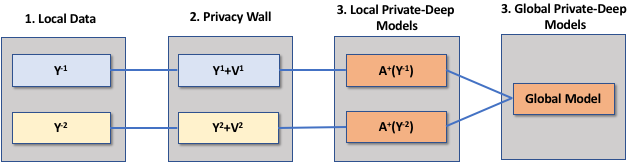
\includegraphics[width=\columnwidth]{images/privacypreserving.png}
\caption{A structural representation of the differentially private distributed learning for deep models.}
\label{fig_structural_representation_distributed_differential_private}
\end{figure}

%\caption{A structural representation of the differentially private distributed learning for deep models.}
%\label{fig_structural_representation_distributed_differential_private}
%\end{figure} 
The distributed form of differentially private deep learning is represented in Fig.~\ref{fig_structural_representation_distributed_differential_private} where a privacy wall is inserted between training data and the globally shared data. The privacy wall uses noise adding mechanisms to attain differential privacy for each participant's private training data. Therefore, the adversaries have no direct access to the training data. 
     





\subsection{Flexible User Authentication}
The Serums user authentication scheme will go beyond traditional "one-size-fits-all" practices towards adopting a personalised and adaptable multi-factor user authentication scheme which will be based on a flexible authentication paradigm, coined FlexPass \cite{belk}, \cite{constantinides}, \cite{hadjidemetriou}. A first conceptual design of the proposed flexible user authentication paradigm is depicted in Figure \ref{fig:flexpass}. Our approach attempts to provide a new user authentication paradigm that leverages upon theories in Cognitive Psychology (dual coding, episodic and semantic memory), which suggest that humans' episodic and semantic memories, represented as verbal and visual information, can be transformed into memorable and personal authentication secrets. Such secrets can be semantically similarly reflected on both textual and graphical password keys, and accordingly used complimentary based on user preference (Figure \ref{fig:flexpass}). The paradigm relies on a single, open-ended, user-selected secret that can be reflected as a textual key and a graphical key. 

\begin{figure}[H]
    \centering
    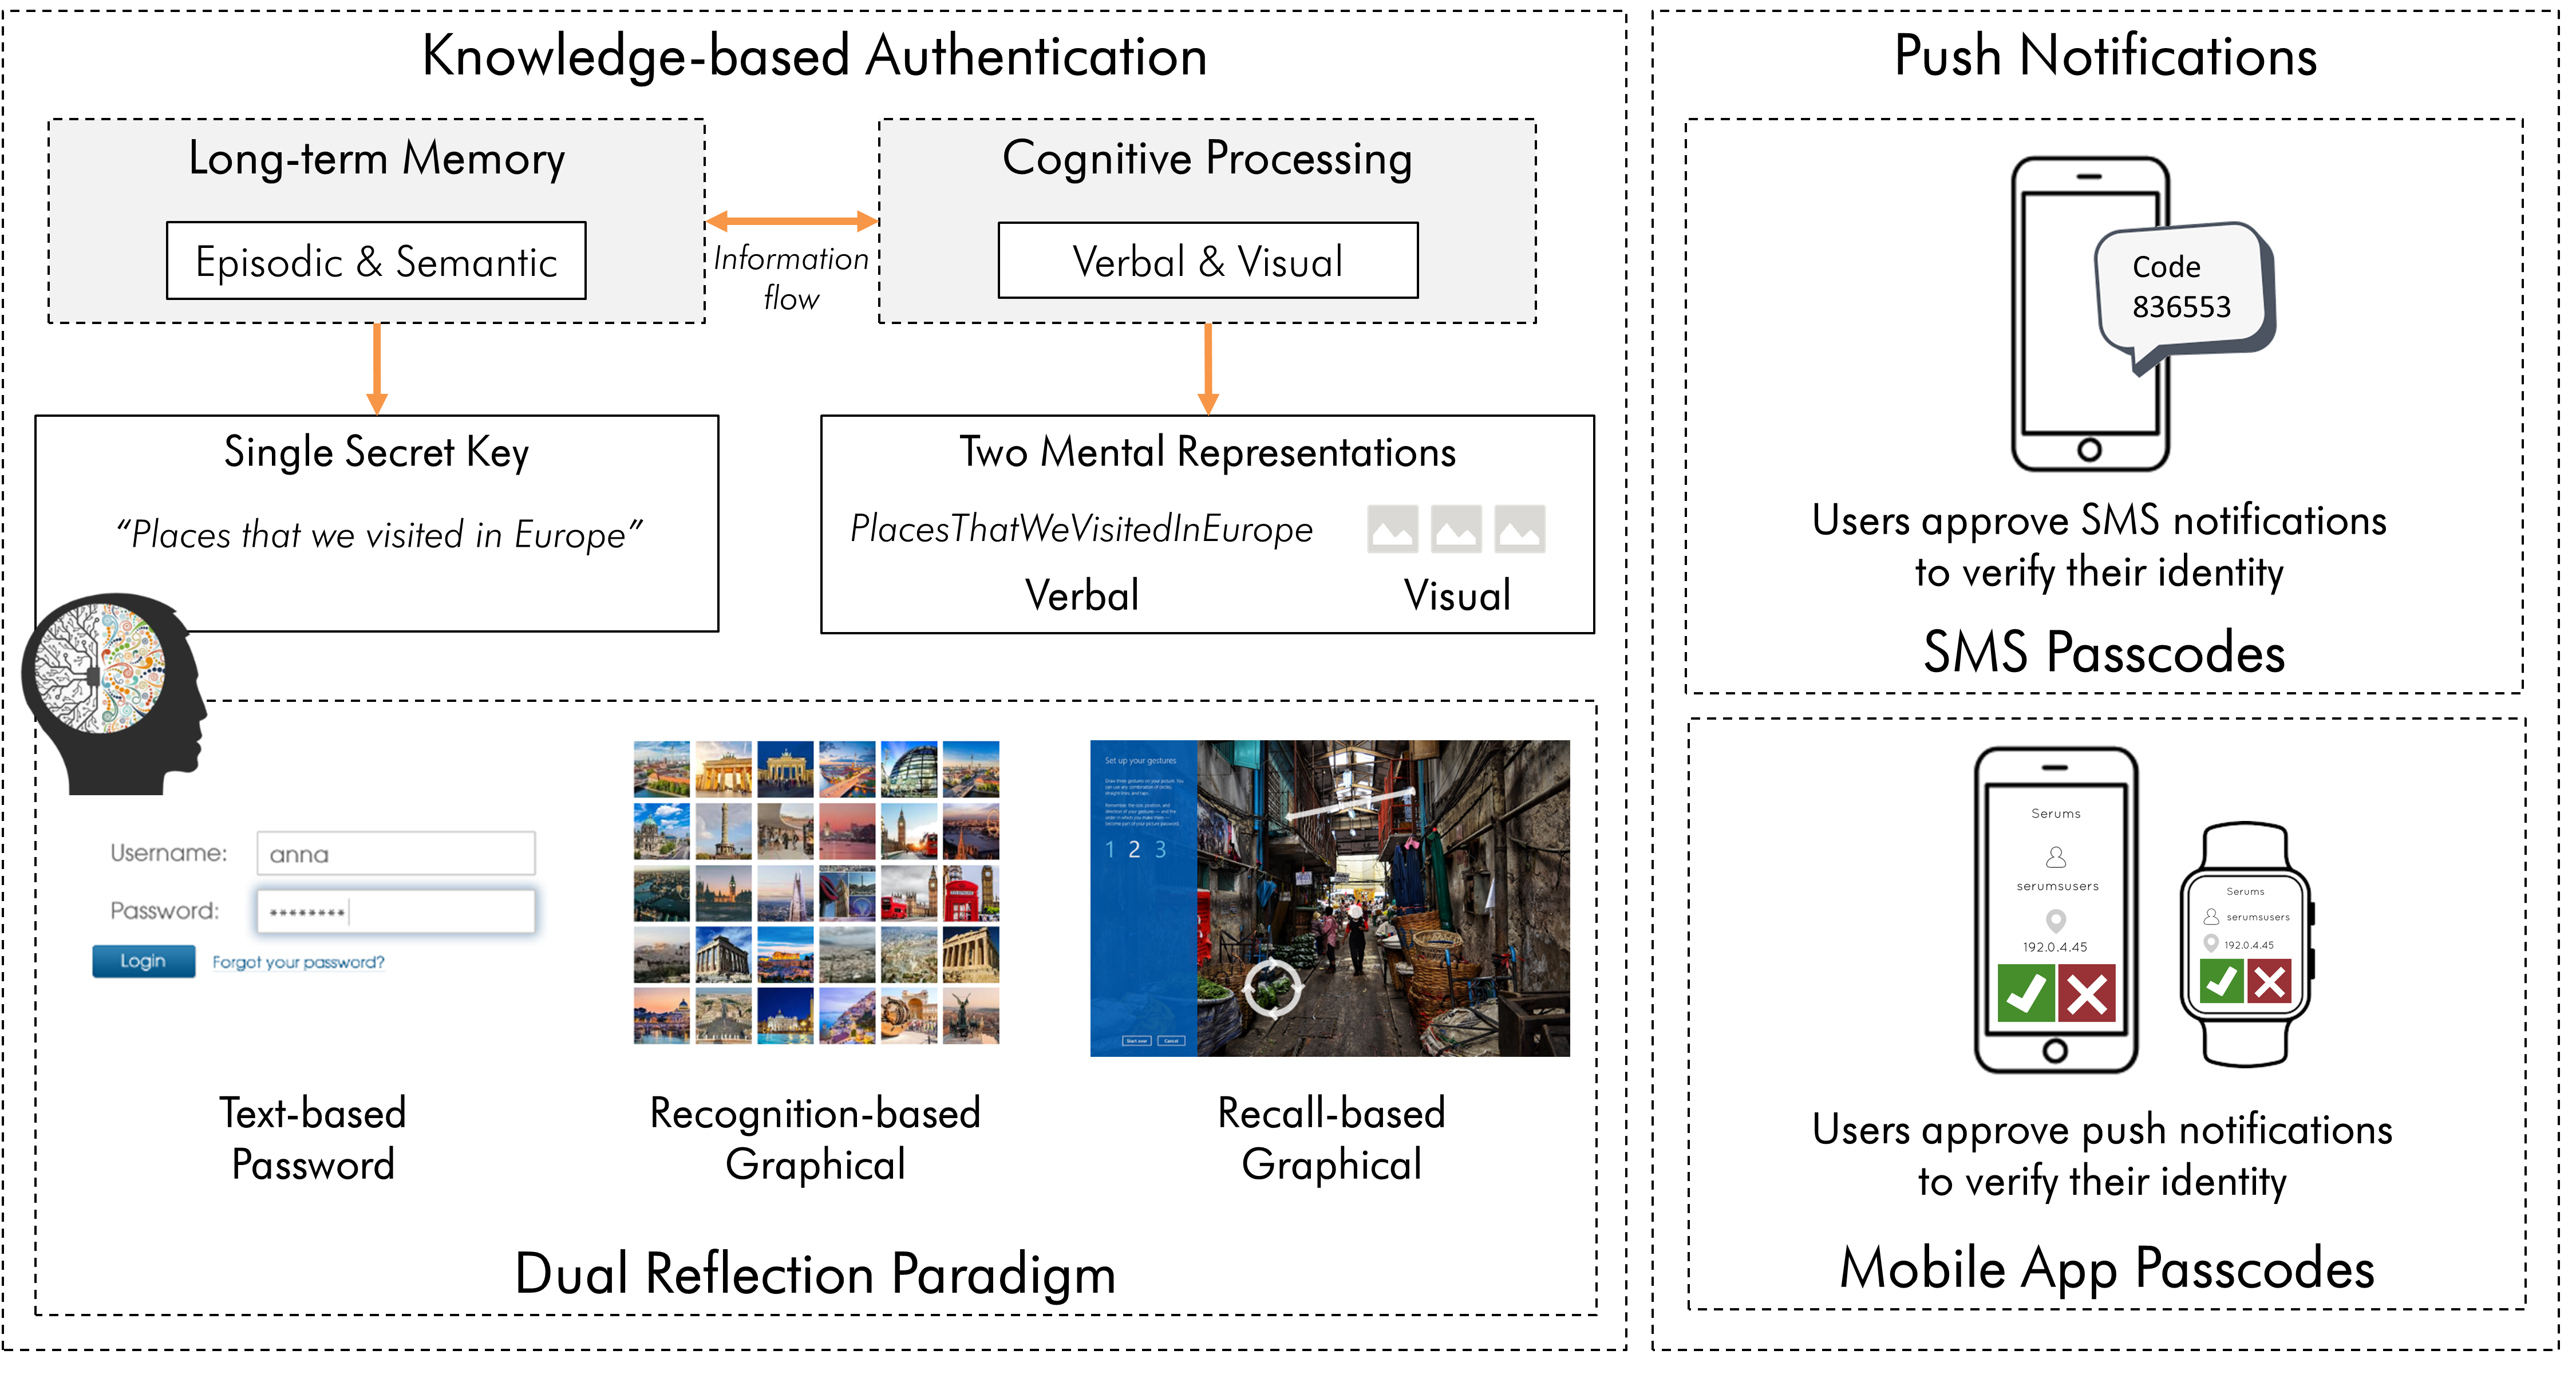
\includegraphics[width=90mm]{images/flexpass.png}
    \caption{Conceptual design of the Flexible User Authentication Paradigm}
    \label{fig:flexpass}
\end{figure}

\textit{Use-case Scenario}. Consider a password creation scenario in which a user chooses a secret derived from his episodic memory, e.g., \textit{Places that we visited in Europe}. In this scenario, the textual password key is based on the articulation of the secret, e.g., the system will generate a textual password key \textit{PlacesThatWeVisitedInEurope}. For the creation of the graphical password key, the user chooses pictures illustrating relevant images through search in Web engines. Other related images from the image search default to decoy images (in the case of recognition-based graphical authentication). Both user-selected and decoy images are finally assigned to the user’s profile to be used for login. Users will also be able to choose a single background image and then draw secret gestures on the image that will be based on the chosen single secret.

Hence, the FlexPass paradigm extends existing works in knowledge-based user authentication based on theories of human cognition with the aim: a) to enhance memorability through ownership, and prior experience and knowledge of each single user; and b) to support user authentication adaptability since users can choose their preferred way to login based on their needs and context of use. For example, users that are on the move and interact on their smartphone might prefer to login with a graphical password, instead of entering text on a virtual keyboard which is considered a demanding and time-consuming task \cite{vonzezschwitz}. The same user however, in a different context, e.g., while at home working on the desktop computer, can choose to login through his textual password key. Note that in both cases, the user is only required to recall the same single secret, which can be reflected differently based on the user’s preference. Similarly, older adults might prefer to always login with a graphical password since they find it easier than textual passwords, as opposed to younger adults that instead, prefer traditional textual passwords \cite{nicholson}.

Nevertheless, the dual nature of FlexPass embraces new vulnerabilities related to security that need closer attention, i.e., a brute-force algorithm could use the additional information provided by the graphical representation to break the textual key. In addition, FlexPass introduces a new kind of observational attack; adversaries know the format of the password and they can see the set of pictures. Accordingly, aiming to add an additional layer of security to the proposed approach, we use a second factor for authentication through push notifications as a first step before proceeding to login. In particular, at a first stage users will be required to approve a push notification that is realised as an SMS notification including an OTP, and a mobile application notification. After verifying their identity, users will login through their preferred user authentication type based on the FlexPass paradigm. Furthermore, the open-ended nature of the suggested paradigm might affect users towards misuse strategies. To assure that users will not create semantically insecure (predictable) grids of images, automated image tagging technologies (e.g., IBM Watson Visual Recognition, Google Vision API, Amazon Rekognition, etc.) and policies need to be investigated to prevent users’ unsafe coping strategies. 
% Need information on Authentication and Authorisation for SERUMS

\subsection{Blockchain}
\textbf{ACC to write the first version}


The access control for the SPHR is handled by Smart Contracts running on Blockchain. The following is the process flow:

\begin{enumerate}
    \item The Hospital (organisation) creates generic access rules about its data, these rules are written in the Blockchain
    \item The Patient creates access rules about this data, these rules are written in the Blockchain
    \item Identifier of the Patient is shared with the data requester
    \item The Doctor authenticates himself
    \item The Doctor (Individual, belonging to a group in an organisation) requests access to data about a Patient (from a Hospital). The Doctor identifier and the Patient identifier are checked against the access rules in the Blockchain (Check/Audit trail)
    \item An access token (or decryption key) is requested from the data vault to access the Patient data
    \item The data vault provides the access token (or decryption key)
    \item A response is sent to the Doctor with access token (or decryption key)
    \item The Doctor requests data about the Patient to the data vault using his access token (or decryption key)
    \item The data vault provides the requested data 
\end{enumerate}

\begin{figure}[H]
    \centering
    
\includegraphics[width=70mm]{images/DataVault/blockchain.png}
    \caption{Process flow for access request}
    \label{fig:blockchain_flow}
\end{figure}



\textbf{ACC to write the first version}


% Need write-up of smart contracts and block chain

\section{Evaluation}

\subsection{Differentially Private Distributed Deep Learning}
Experiments have been made on benchmark datasets to 1) study the effect of privacy level on the classification accuracy of the proposed method; 2) compare the proposed noise adding mechanism with the classical Gaussian mechanism in terms of classification accuracy; 3) compare the non-private version of the proposed distributed deep fuzzy models based classifier with the classical machine learning methods in classifying high-dimensional data.   

\subsubsection{MNIST dataset}
The method is studied by considering a handwritten digits recognition problem with the widely used MNIST dataset. The dataset contains $28 \times 28$ sized images divided into training set of 60000 images and testing set of 10000 images. The images' pixel values were divided by 255 to normalize the values in the range from $0$ to $1$. The $28 \times 28$ normalized values of each image are flattened to an equivalent $784-$dimensional data vector.

To create a scenario for distributed learning, each class's training dataset was partitioned into $S$ number of data-subsets using $k-$means clustering and $S$ was chosen as $S =\lceil N/1000 \rceil$. Each data-subset is assumed private and the method's $(\epsilon,\delta)-$differential privacy against perturbation (in one element of data vector), with perturbation magnitude upper bounded by $d = 1$, is considered.
\begin{figure}
\centerline{ \subfigure[$\delta = 1\mathrm{e}{-6}$.]{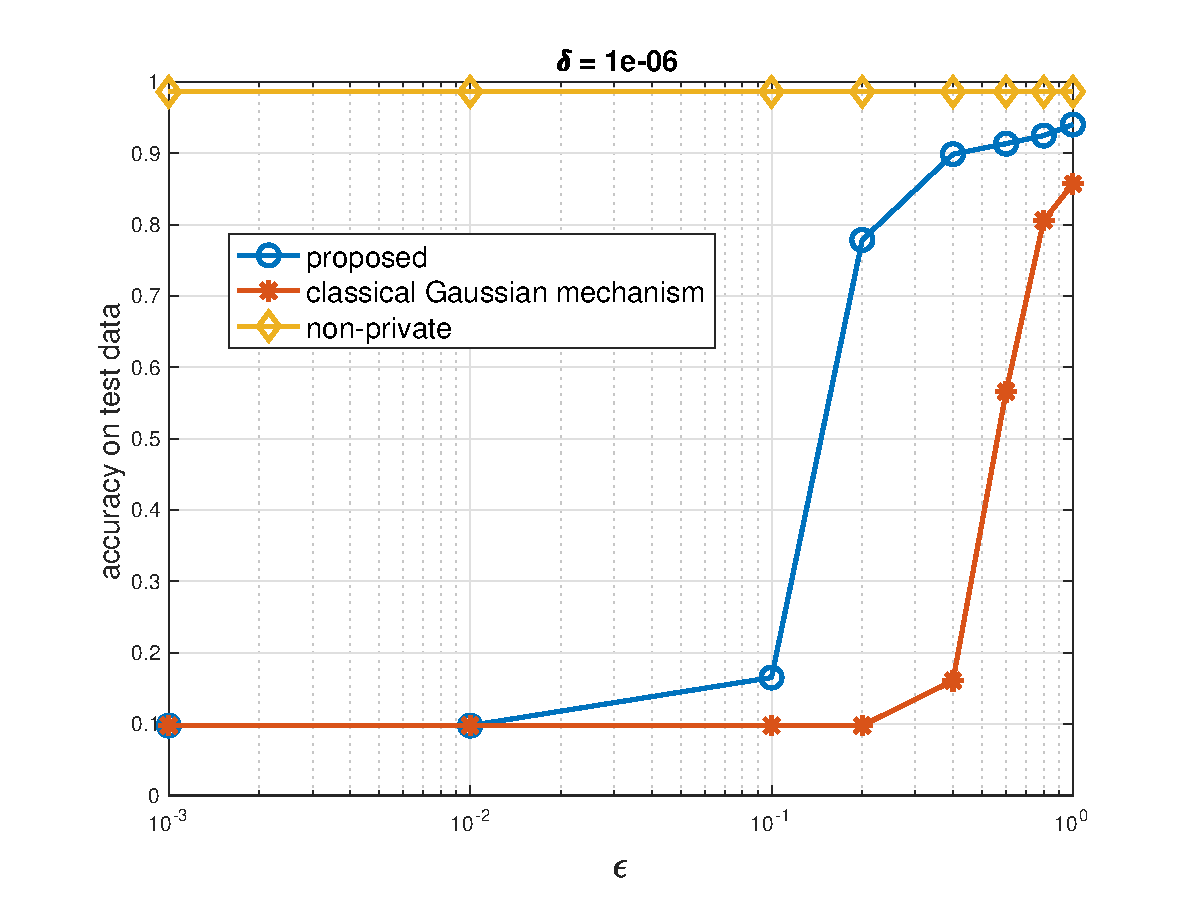
\includegraphics[width = 1.5in]{images/M_1}\label{fig_M_1}} \hfil \subfigure[$\delta = 1\mathrm{e}{-5}$.]{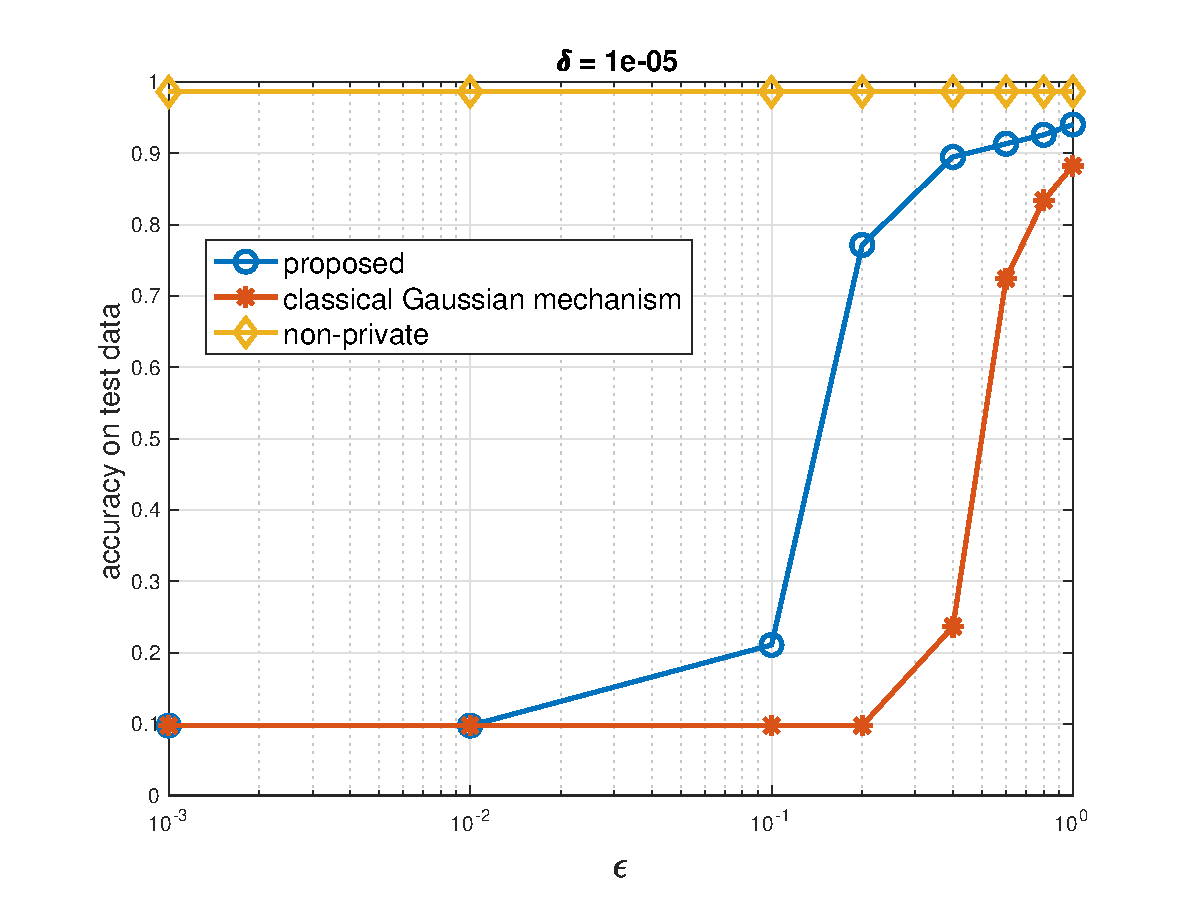
\includegraphics[width = 1.5in]{images/M_2}\label{fig_M_2}}}
\centerline{ \subfigure[$\delta = 1\mathrm{e}{-4}$.]{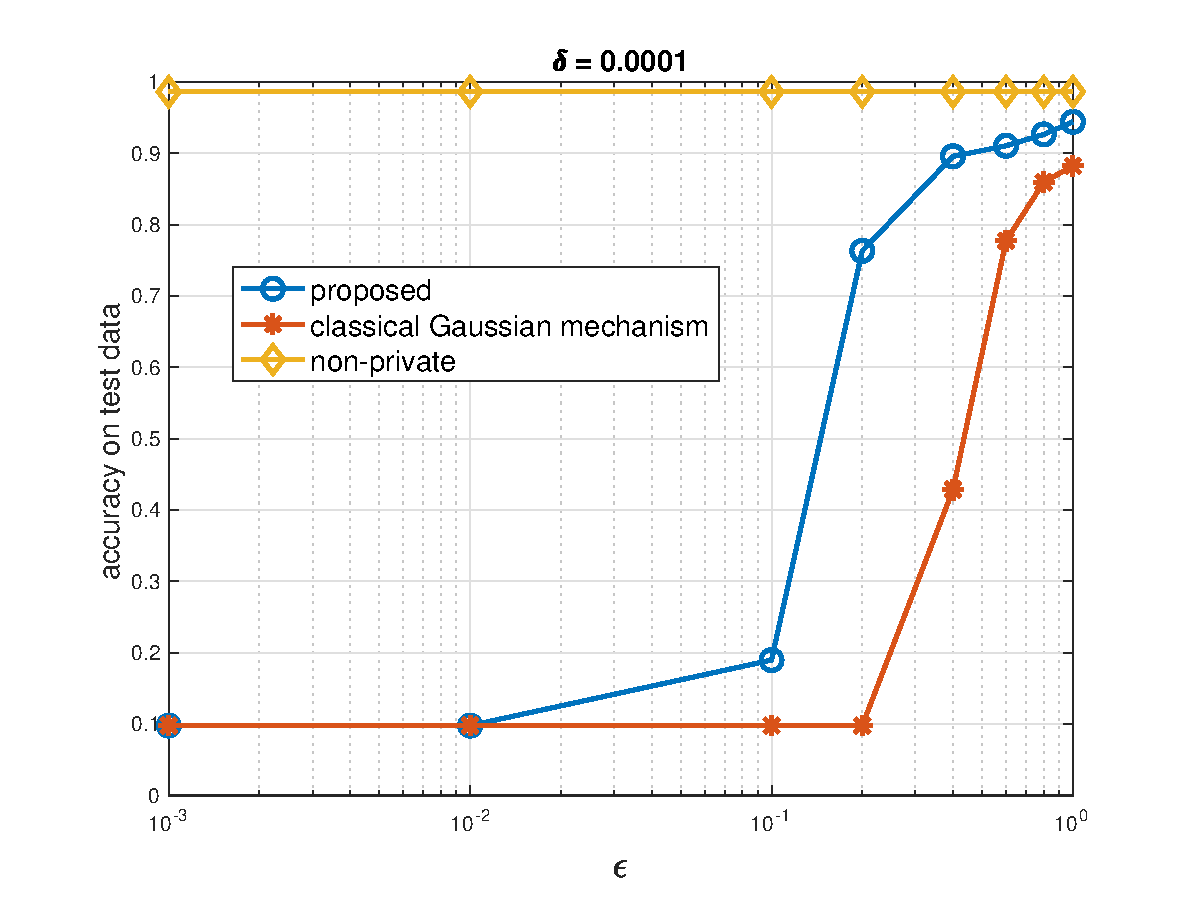
\includegraphics[width = 1.5in]{images/M_3}\label{fig_M_3}} \hfil \subfigure[$\delta = 1\mathrm{e}{-3}$.]{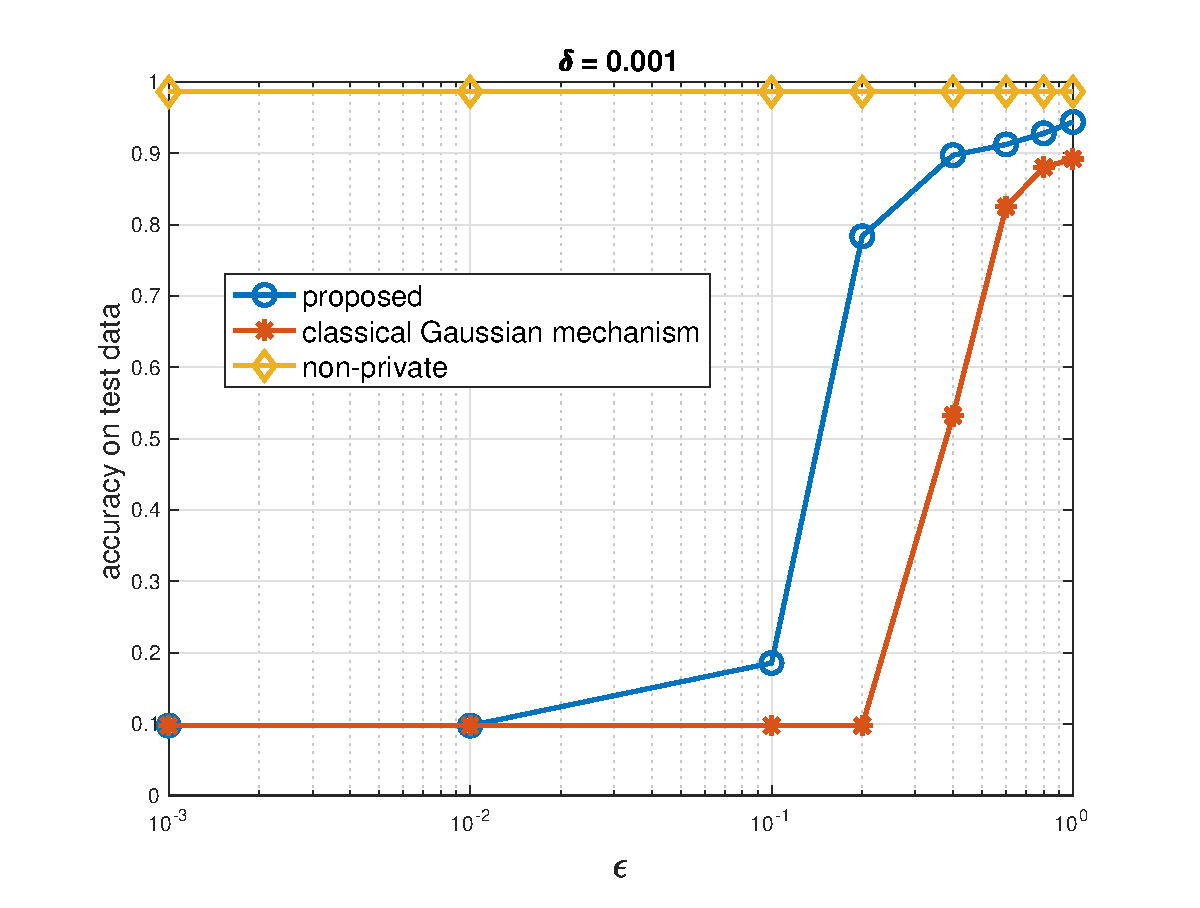
\includegraphics[width = 1.5in]{images/M_4}\label{fig_M_4}}}
\centerline{ \subfigure[$\delta = 1\mathrm{e}{-2}$.]{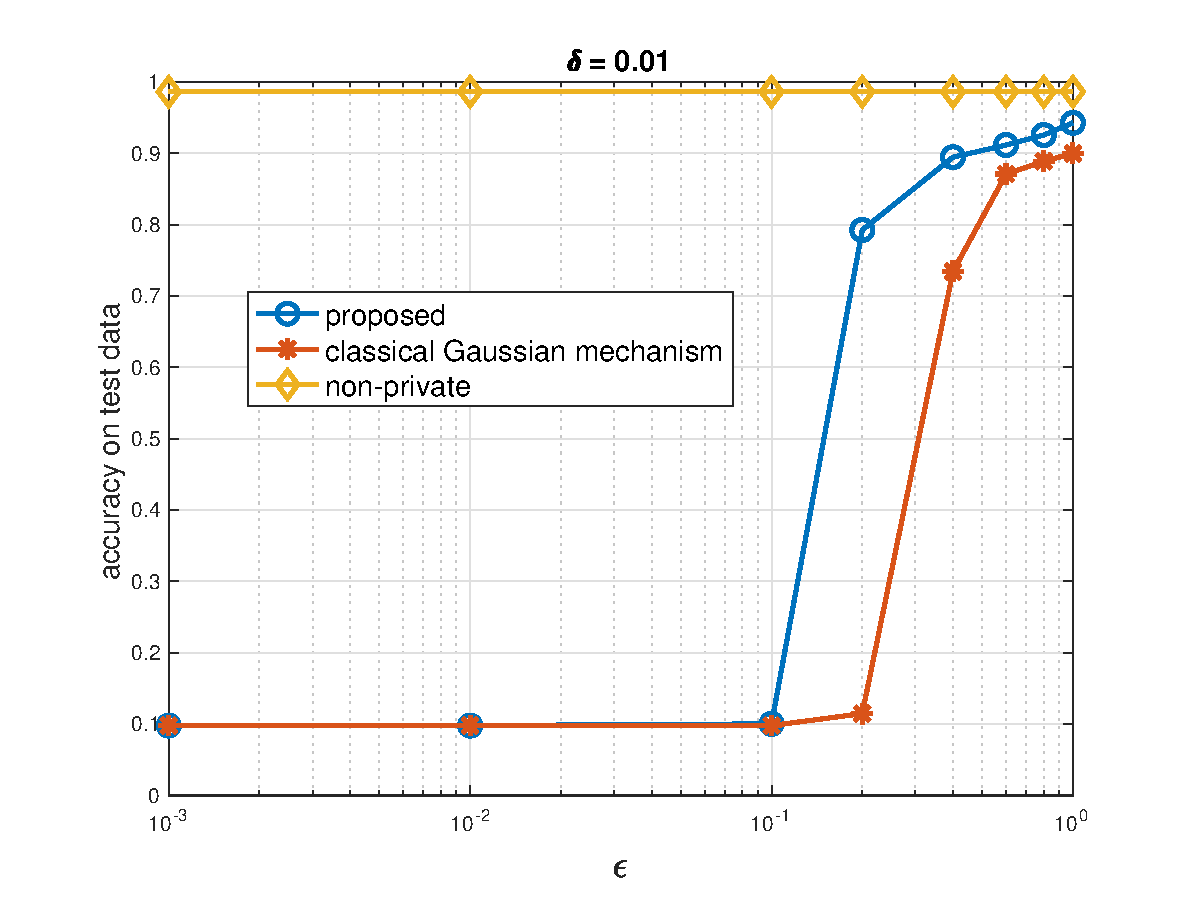
\includegraphics[width = 1.5in]{images/M_5}\label{fig_M_5}} \hfil \subfigure[$\delta = 1\mathrm{e}{-1}$.]{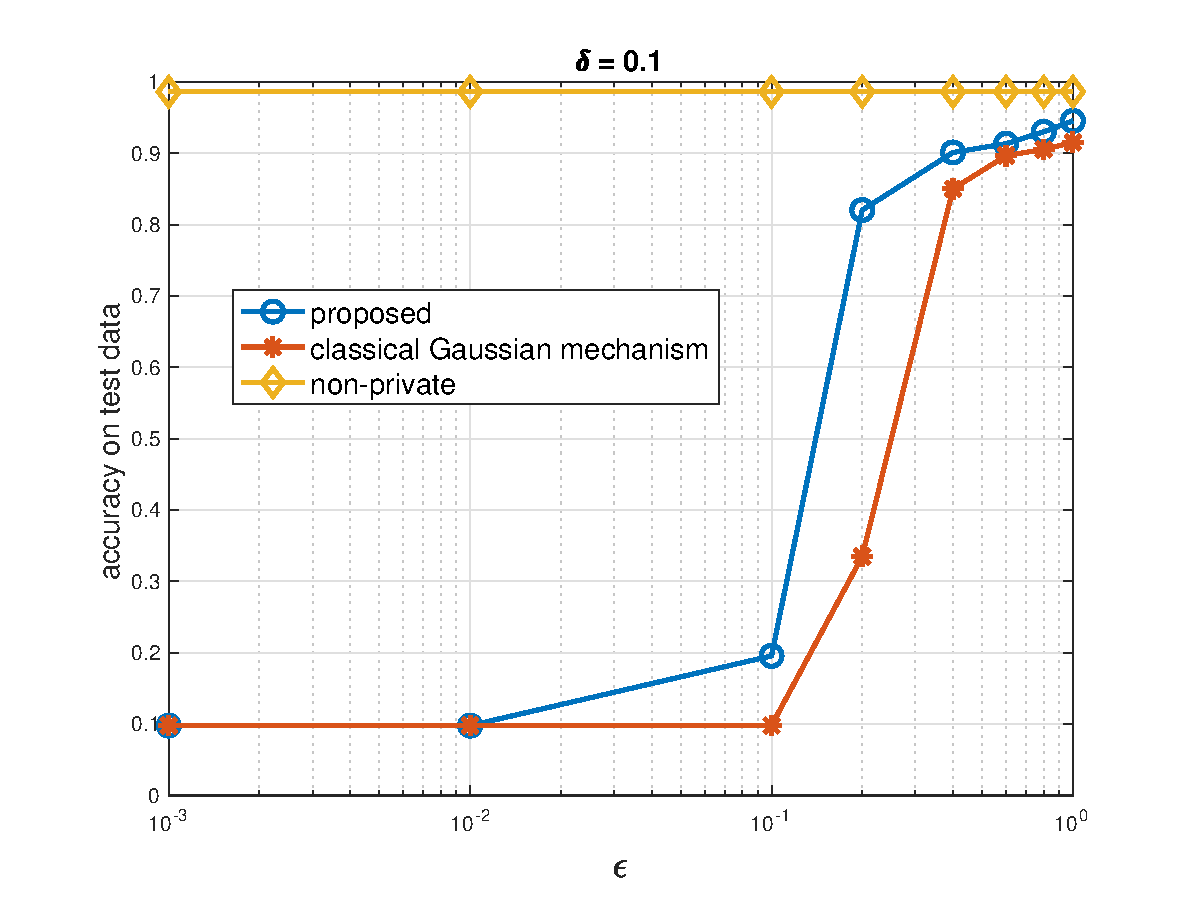
\includegraphics[width = 1.5in]{images/M_6}\label{fig_M_6}}}
\centerline{ \subfigure[$\delta = 0.5$.]{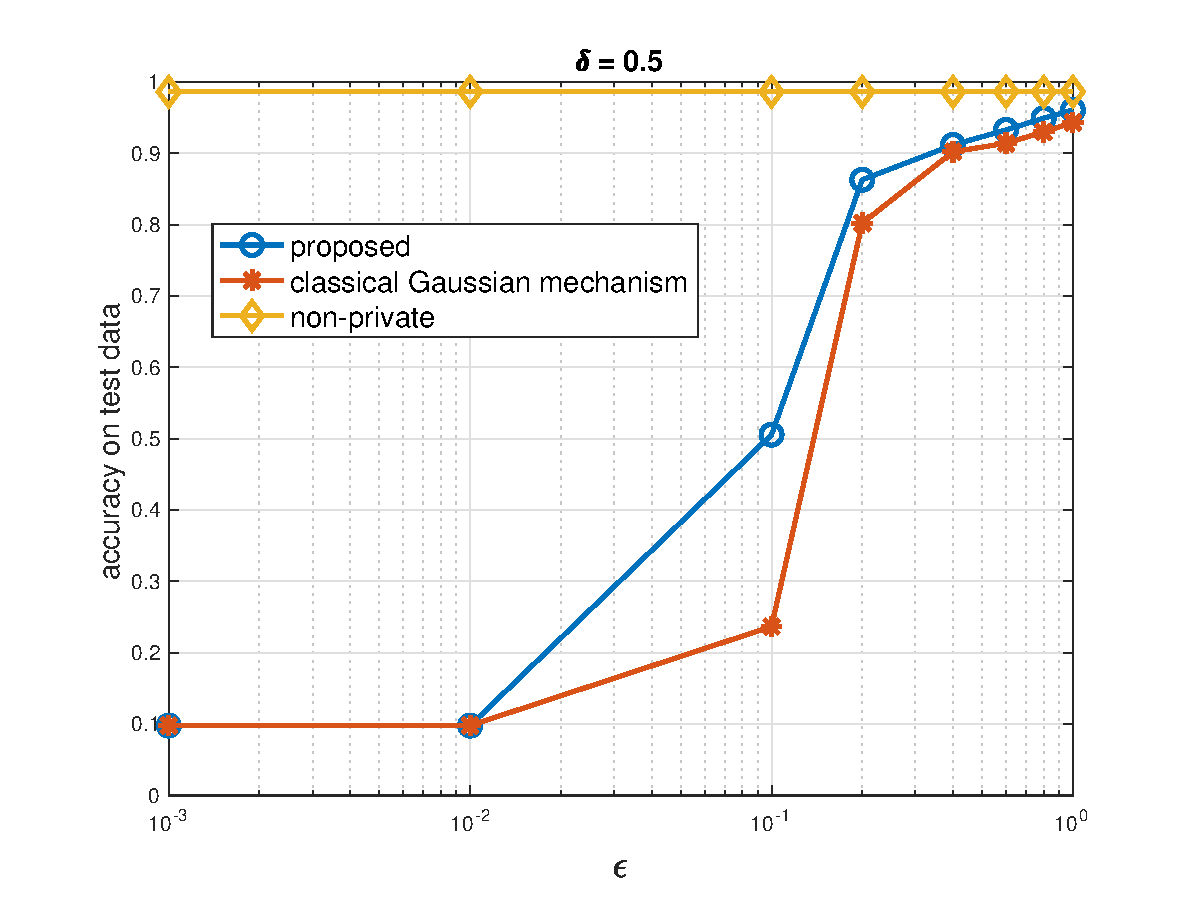
\includegraphics[width = 1.5in]{images/M_7}\label{fig_M_7}} \hfil \subfigure[$\delta = 0.9$.]{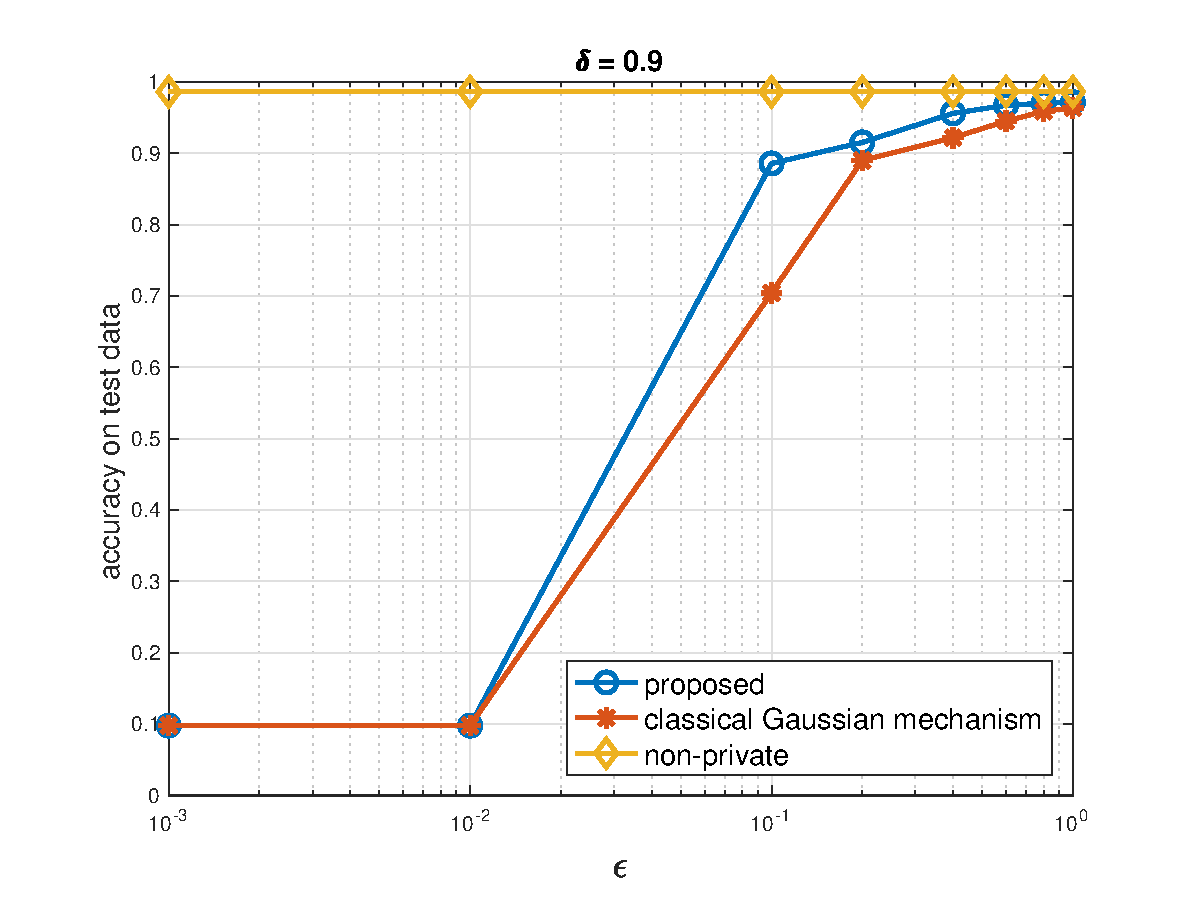
\includegraphics[width = 1.5in]{images/M_8}\label{fig_M_8}}}
\caption{The effect of $\epsilon$ on MNIST test data classification accuracy.}\label{fig_M_first_part}
\end{figure}
\begin{figure}
\centerline{ \subfigure[$\epsilon = 1\mathrm{e}{-3}$.]{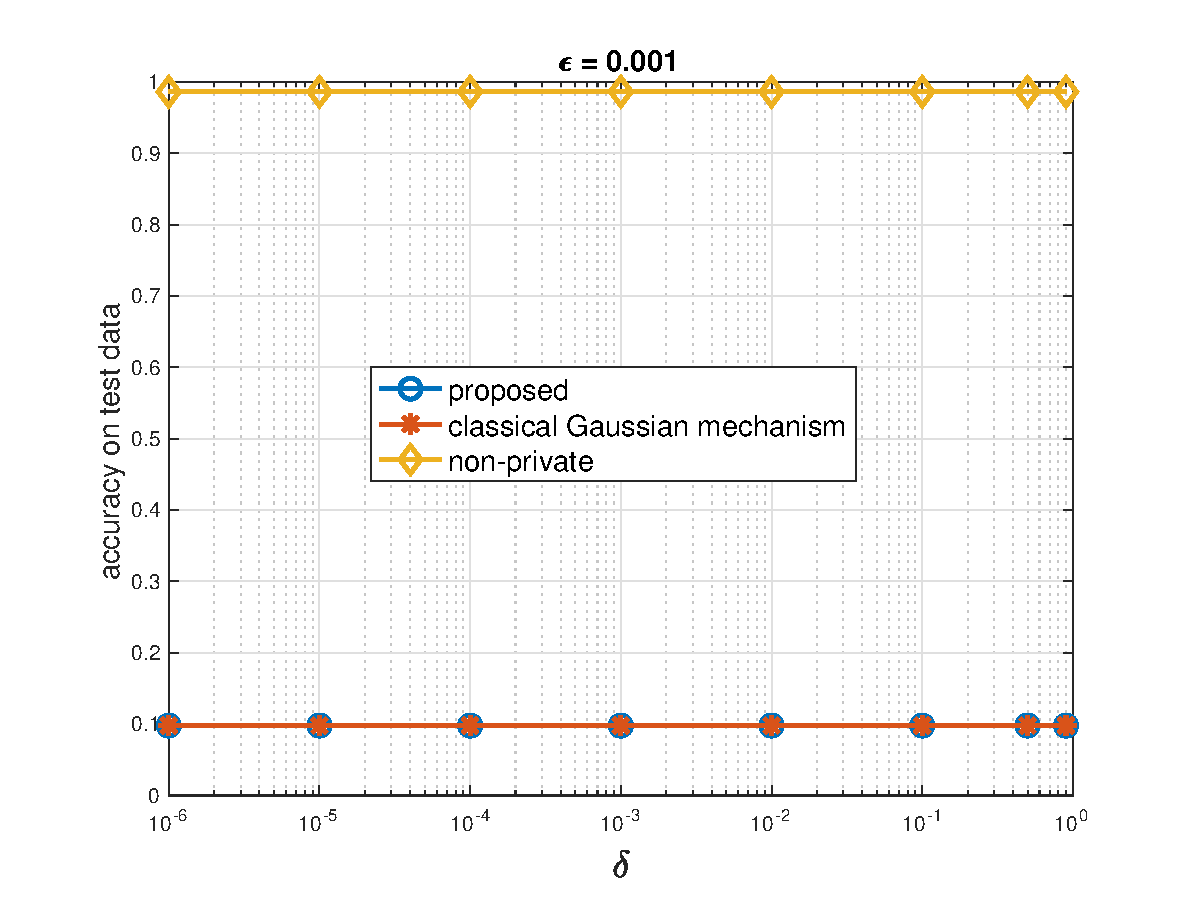
\includegraphics[width = 1.5in]{images/M_9}\label{fig_M_9}} \hfil \subfigure[$\epsilon = 1\mathrm{e}{-2}$.]{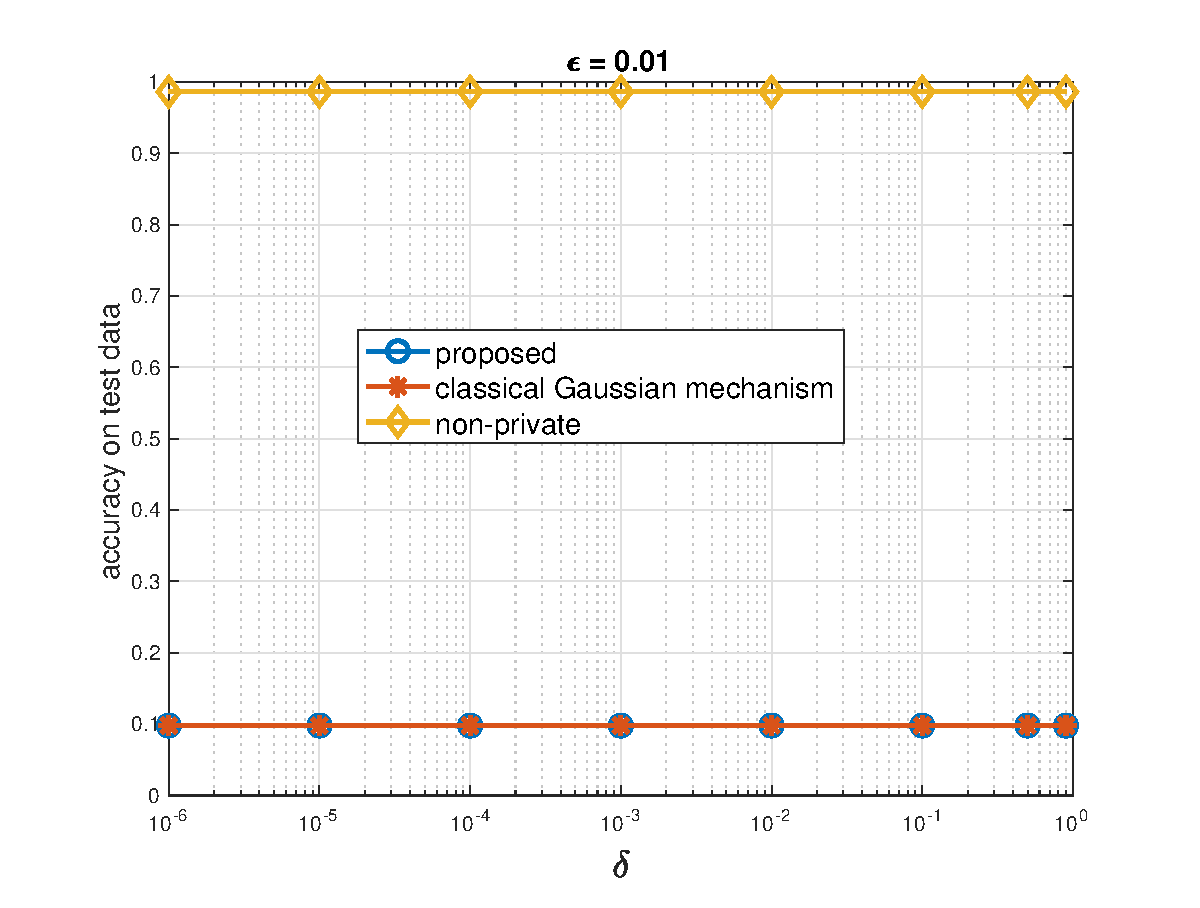
\includegraphics[width = 1.5in]{images/M_10}\label{fig_M_10}}}
\centerline{ \subfigure[$\epsilon = 1e-1$.]{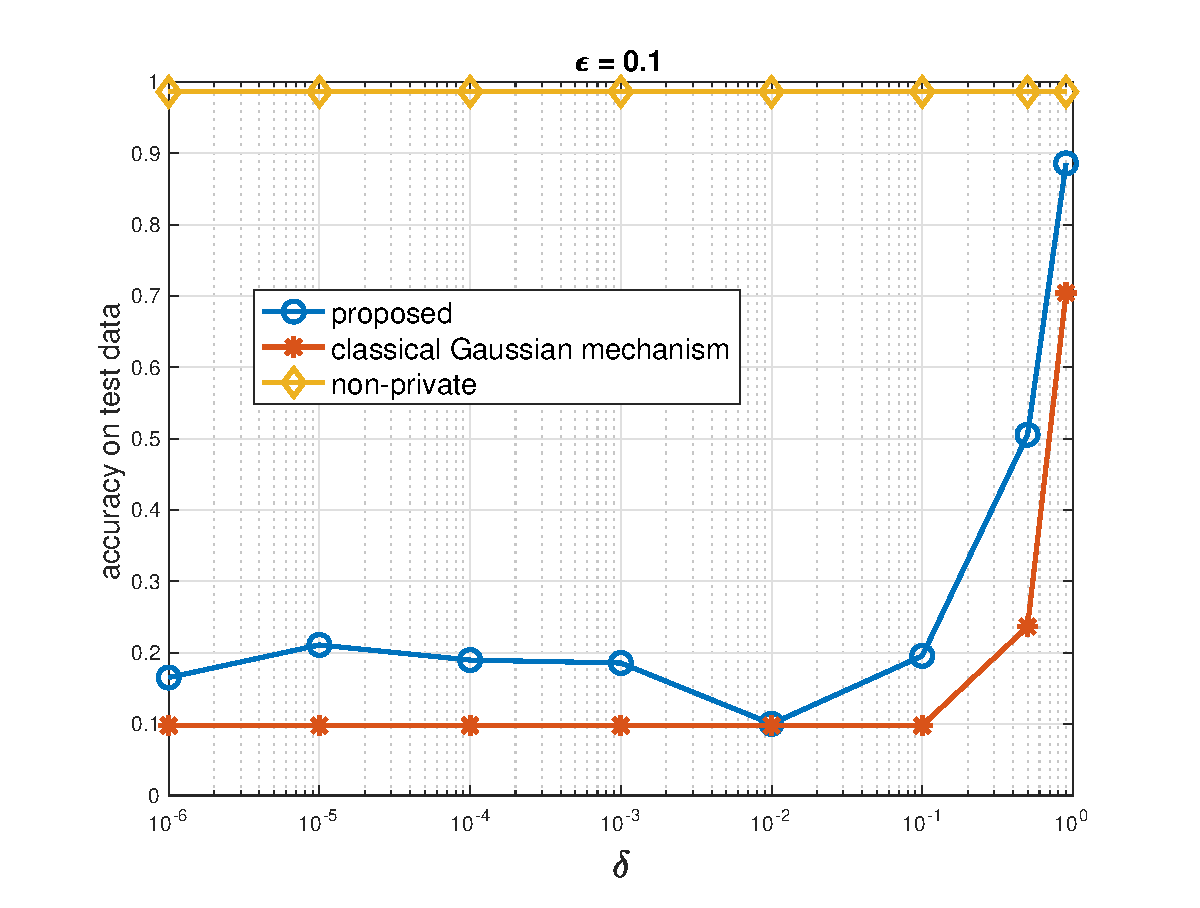
\includegraphics[width = 1.5in]{images/M_11}\label{fig_M_11}} \hfil \subfigure[$\epsilon = 0.2$.]{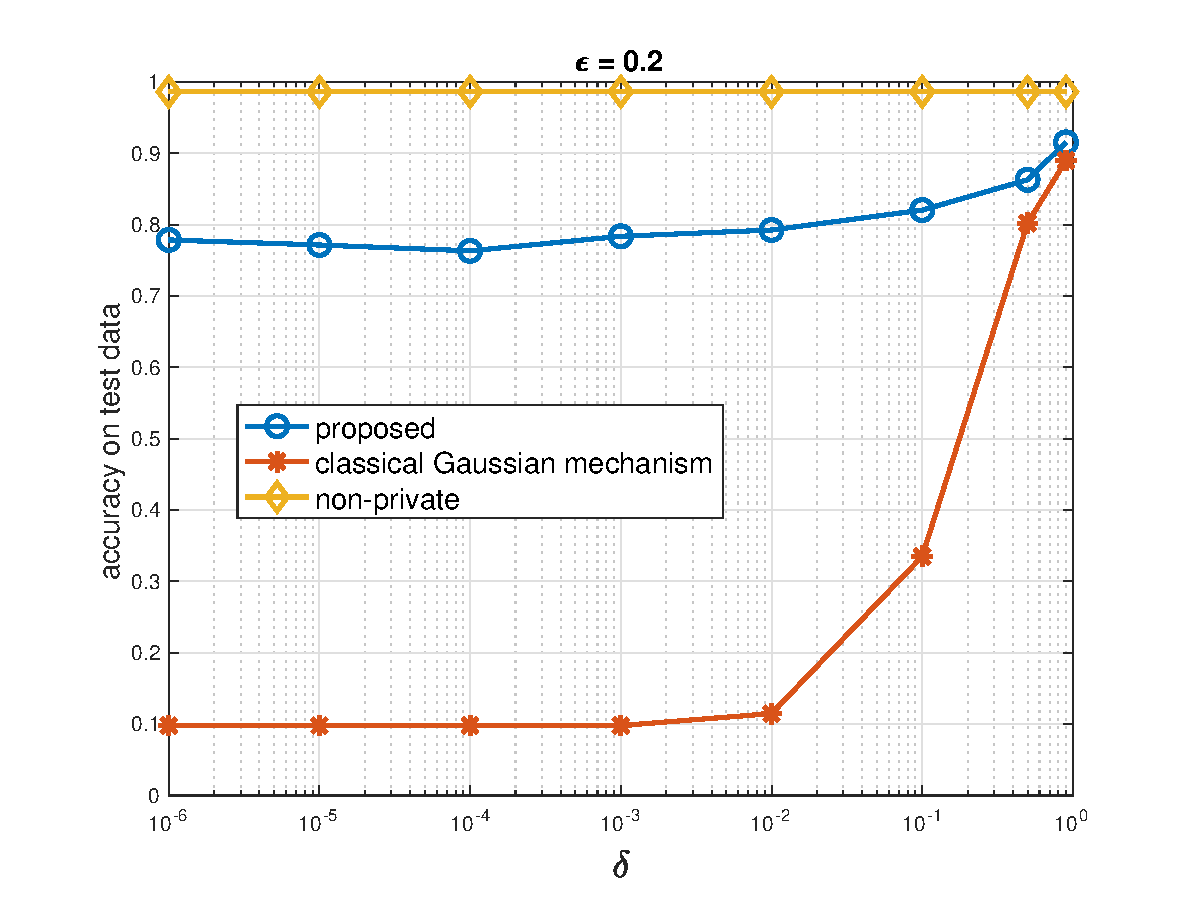
\includegraphics[width = 1.5in]{images/M_12}\label{fig_M_12}}}
\centerline{ \subfigure[$\epsilon = 0.4$.]{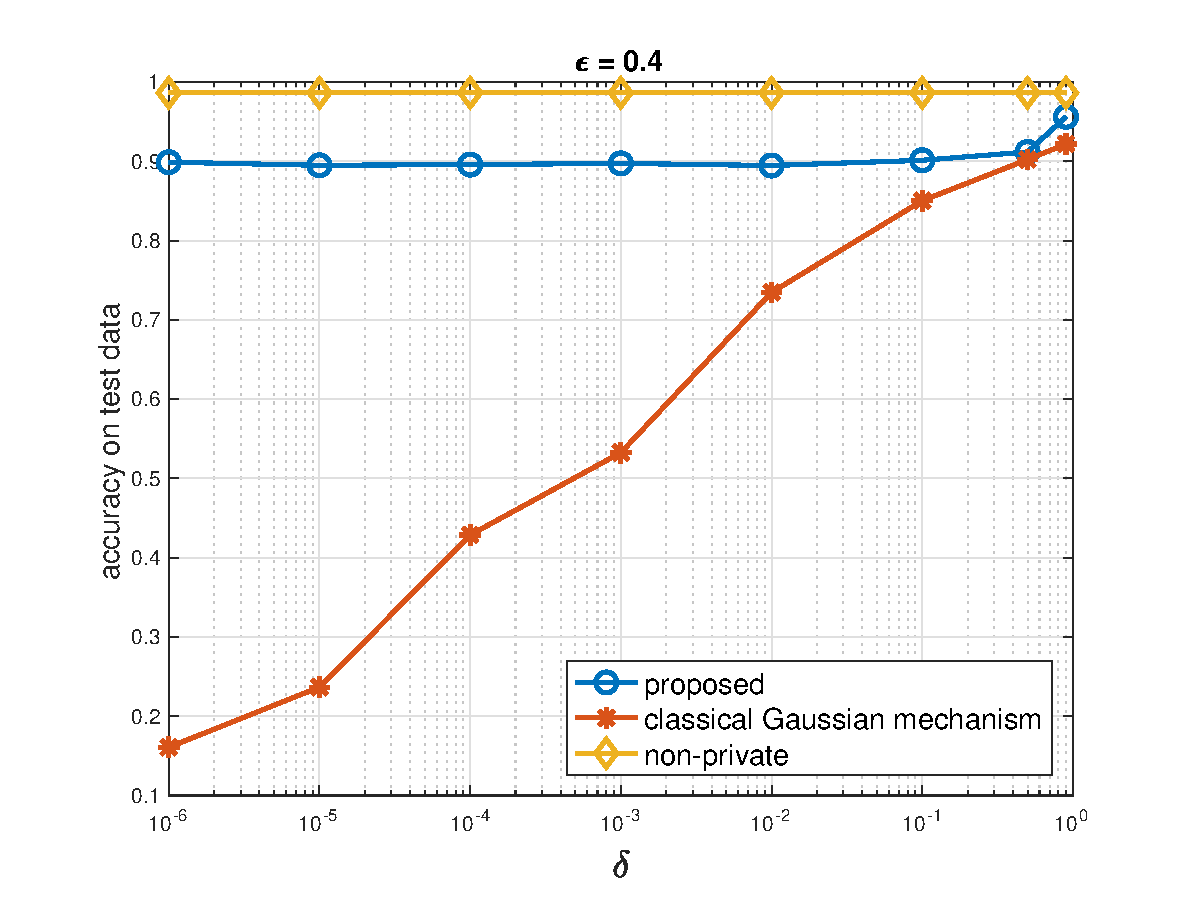
\includegraphics[width = 1.5in]{images/M_13}\label{fig_M_13}} \hfil \subfigure[$\epsilon = 0.6$.]{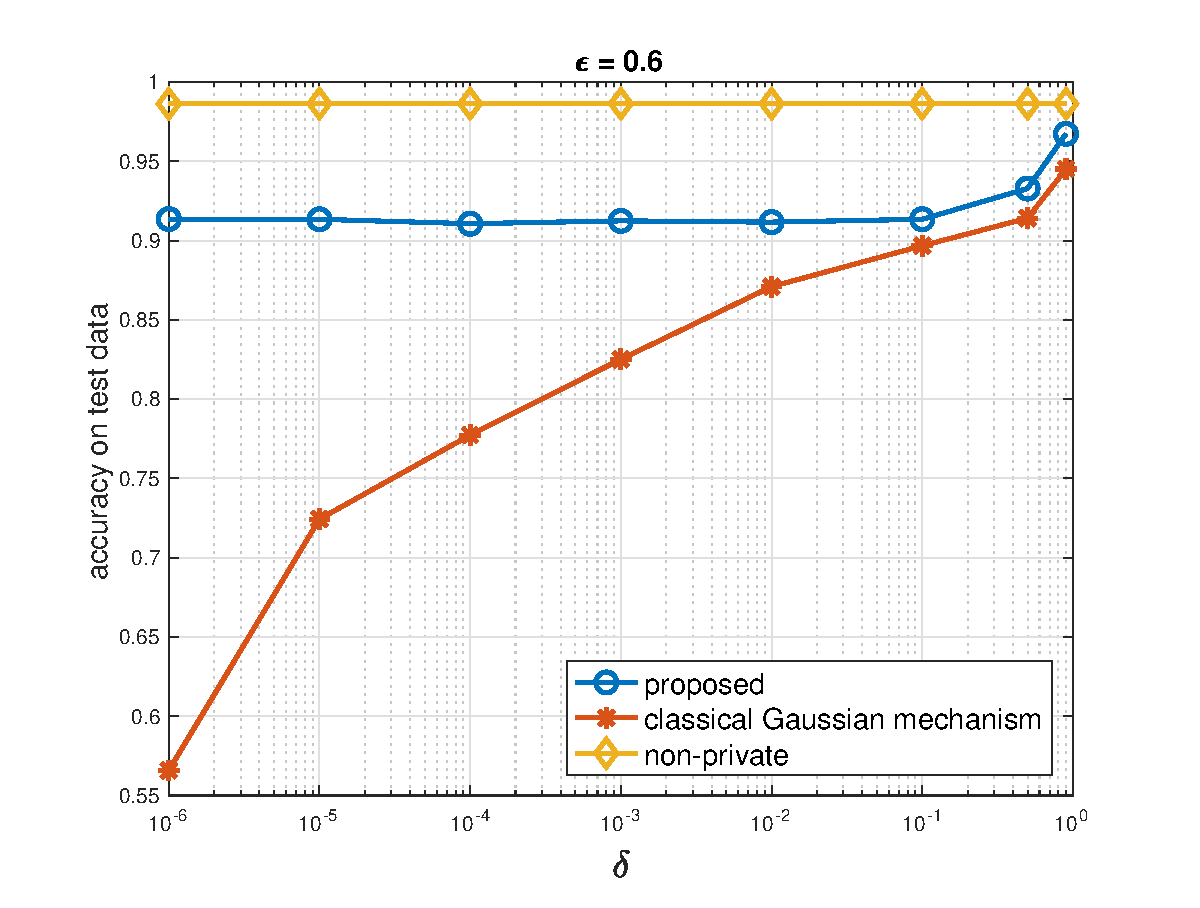
\includegraphics[width = 1.5in]{images/M_14}\label{fig_M_14}}}
\centerline{ \subfigure[$\epsilon = 0.8$.]{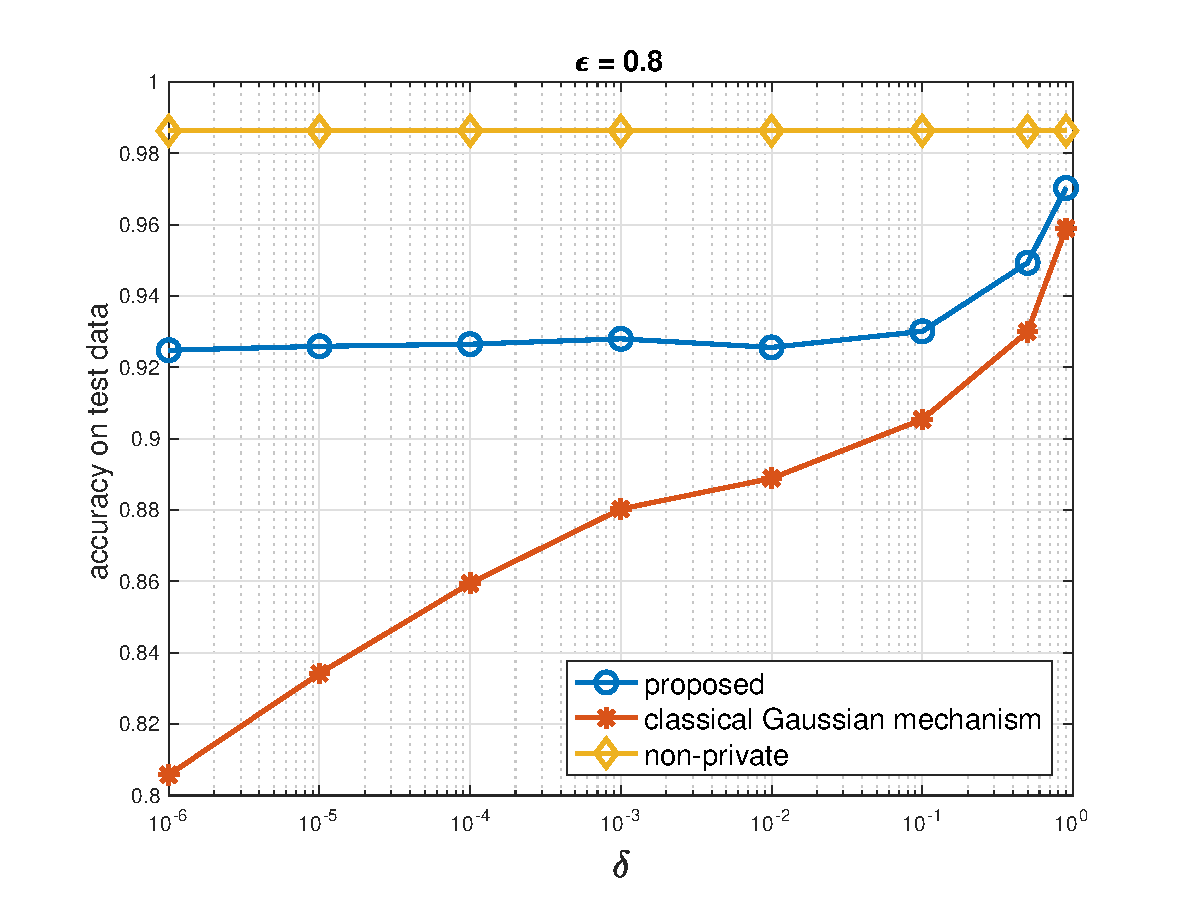
\includegraphics[width = 1.5in]{images/M_15}\label{fig_M_15}} \hfil \subfigure[$\epsilon = 1$.]{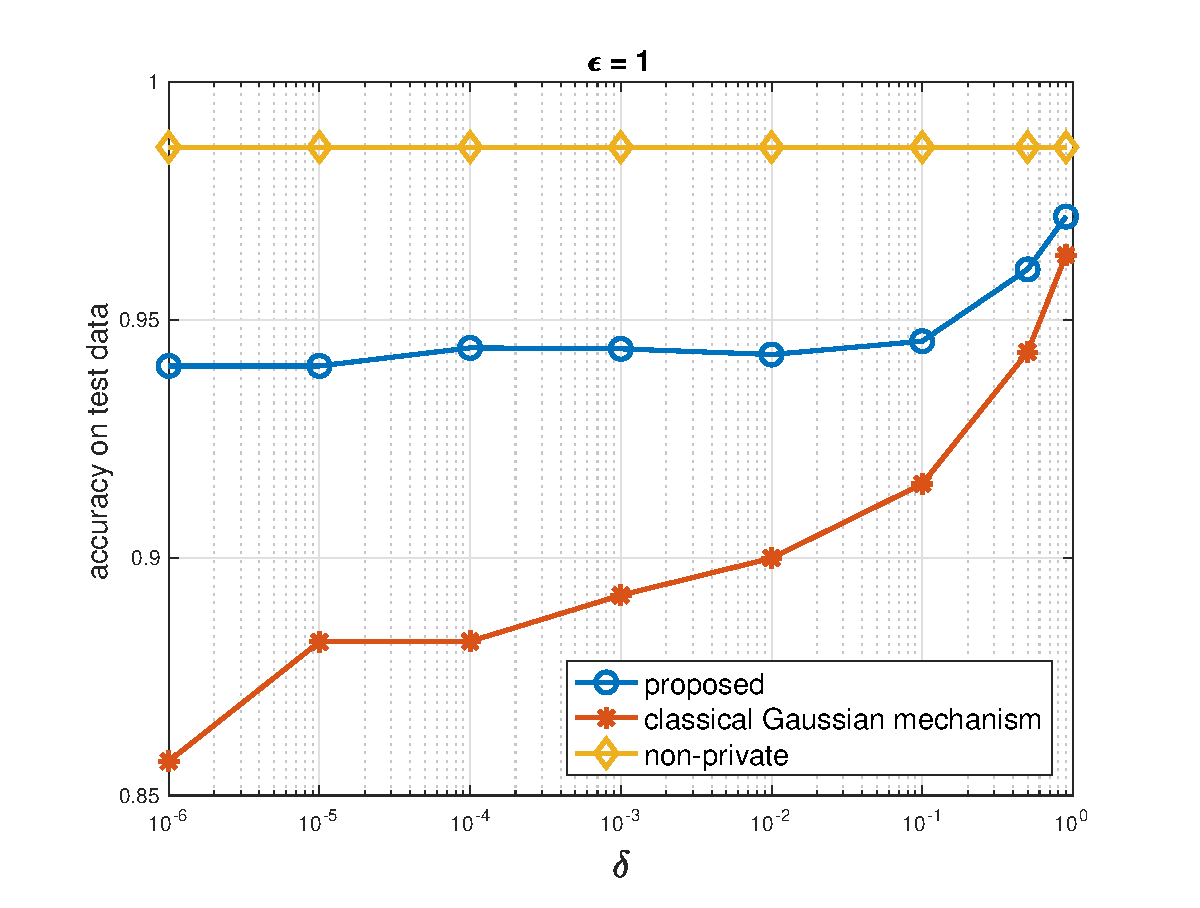
\includegraphics[width = 1.5in]{images/M_16}\label{fig_M_16}}}
\caption{The effect of $\delta$ on MNIST test data classification accuracy.}\label{fig_M_second_part}
\end{figure}

Numerous experiments are made to study the effect of $\epsilon$ and $\delta$ on the accuracy in classifying test images. The non-private version of the proposed method is applied to calculate the reference performance of the method. The experimental results have been displayed in Fig.~\ref{fig_M_first_part} and Fig.~\ref{fig_M_second_part}. The following inferences are drawn from the results: 1) The proposed method consistently achieves a higher accuracy than the classical Gaussian mechanism. This is observed in all subfigures of Fig.~\ref{fig_M_first_part} and Fig.~\ref{fig_M_second_part} except in Fig.~\ref{fig_M_9} and Fig.~\ref{fig_M_10} where both mechanisms perform nearly the same. 2) In very-high privacy regime (i.e. when $\epsilon \leq 1\mathrm{e}{-2}$ for this particular dataset), the noise level is so high that the optimality of the proposed mechanism doesn't manifest itself to any observed gain in the accuracy. This should explain the nearly same performance of both mechanism in Fig.~\ref{fig_M_9} and Fig.~\ref{fig_M_10}. 

To study the robustness, the test images are contaminated by zero-mean Gaussian additive noise with varying level of standard deviation. The widely used Convolutional Neural Network (CNN) is taken as a reference for comparing the performance. A CNN with the patch size of $5 \times 5$, first convolutional layer of 32 features, second convolutional layer of 64 features, and densely connected layer of 1024 neurons is considered. The convolutions use a stride of one and are zero padded. The pooling is max pooling over $2\times2$ blocks. The CNN was trained for 10000 iterations where each iteration uses a batch size of 100 images. 
\begin{table}
\renewcommand{\arraystretch}{1.3}
\caption{The effect of noise level on the performance in classifying MNIST digits}
\label{table_robustness_results} \centering
\begin{tabular}{c||*{2}{c}}
\hline
\bfseries $\begin{array}{c} \mbox{noise} \\ \mbox{standard deviation} \end{array}$ & \multicolumn{2}{c}{\bfseries classification accuracy on test images}  \\
\cline{2-3} 
 & \bfseries proposed  &    \bfseries CNN  \\ 
\hline \hline  
0 & 0.9863    & \textbf{0.9897}  \\
0.2 &   \textbf{0.9825}   & 0.9608  \\ 
0.4 & \textbf{0.9630}  & 0.8198 \\ 
0.6 & \textbf{0.9019}   & 0.6227  \\ 
0.8 & \textbf{0.7818}  & 0.4482  \\
1 & \textbf{0.6335}  & 0.3203 \\
\hline \hline
\end{tabular}
\end{table} 

Table~\ref{table_robustness_results} lists the performance of non-private version of the proposed method. The robustness of the proposed approach is clearly observed in Table~\ref{table_robustness_results} as with an increasing level of noise the decrease in classification accuracy is observed to be much slower in the case of proposed method than CNN. 

\subsubsection{Freiburg Groceries Dataset}
The image category classification problem is considered using ``Freiburg Groceries Dataset''~\cite{DBLP:journals/corr/JundAEB16} to study the privacy of the proposed method and to compare it with the classical machine learning algorithms. The dataset~\cite{DBLP:journals/corr/JundAEB16} contains around 5000 labeled images of grocery products commonly sold in Germany. The images have been categorized into 25 different classes of grocery products. A feature vector is created from each image by extracting features from ``AlexNet'' and ``VGG-16'' networks which are pre-trained Convolutional Neural Networks. The activations of the fully connected layer ``fc6'' in AlexNet constitute a $4096-$dimensional feature vector. Similarly, the activations of the fully connected layer ``fc6'' in VGG-16 constitute another $4096-$dimensional feature vector. The features extracted by both networks are joined together to form a $8192-$dimensional vector. The complete set of feature vectors is normalized to have zero-mean and unity-variance along each dimension.  

We choose a training-testing data split and a distributed learning scenario was created assuming that a class's complete training data is owned by a single participant. Thus the number of participants is equal to the number of classes. Several experiments have been made to study the method's $(\epsilon,\delta)-$differential privacy against perturbation (in one element of data vector), with perturbation magnitude upper bounded by $d = 0.1$. Also, the non-private version of our method is compared with the following machine learning techniques: 1) $k$-nearest neighbor ($k$-NN) with $k = 1$; 2) Naive Bayes; 3) Decision Tree; 4) Support Vector Machine (SVM); 5) Ensemble Learning via Boosting 100 Classification Trees; 6) Random Forest of 100 Classification Trees. 

Table~\ref{table_results_grocery_images}, Fig.~\ref{fig_G_first_part}, and Fig.~\ref{fig_G_second_part} state the experimental results. The following inferences are drawn from the obtained results: 1) A higher accuracy of the proposed method in comparison to Gaussian mechanism is consistently observed in all subfigures of Fig.~\ref{fig_G_first_part} and Fig.~\ref{fig_G_second_part} except in Fig.~\ref{fig_G_9} where both mechanisms perform nearly same. 2) In very-high privacy regime (i.e. when $\epsilon \leq 1\mathrm{e}{-3}$ for this particular dataset), the noise level is so high that the optimality of the proposed mechanism doesn't manifest itself to any observed gain in the accuracy. This should explain the nearly same performance of both mechanism in Fig.~\ref{fig_G_9}. 3) Also in very-low privacy regime, e.g. in Fig.~\ref{fig_G_16} at higher $\delta$ values, the noise level is so low that the both mechanism perform nearly the same. 4) A better performance of the proposed fuzzy based method in comparison to classical machine learning methods is observed (in Table~\ref{table_results_grocery_images}) in classifying high-dimensional data vectors. 
\begin{table}
\renewcommand{\arraystretch}{1.3}
\caption{Results of experiments on Freiburg groceries dataset}
\label{table_results_grocery_images} \centering
\begin{tabular}{c||c}
\hline
\bfseries method  & \bfseries testing accuracy in \%   \\
\hline \hline  
$(0.1,1\mathrm{e}{-6})-$differentially private proposed & \textbf{78.88} \\
$(0.1,1\mathrm{e}{-6})-$differentially private Gaussian & 42.53 \\
Non-private proposed &  \textbf{88.50} \\
Non-private $1$-NN & 78.00      \\
Non-private SVM & 77.90      \\
Non-private Random Forest &  63.17   \\
Non-private Naive Bayes & 56.78    \\
Non-private Ensemble Learning & 38.31     \\
Non-private Decision Tree & 31.34   \\
\hline \hline
\end{tabular}
\end{table} 
\begin{figure}[!h]
\centerline{ \subfigure[$\delta = 1\mathrm{e}{-6}$.]{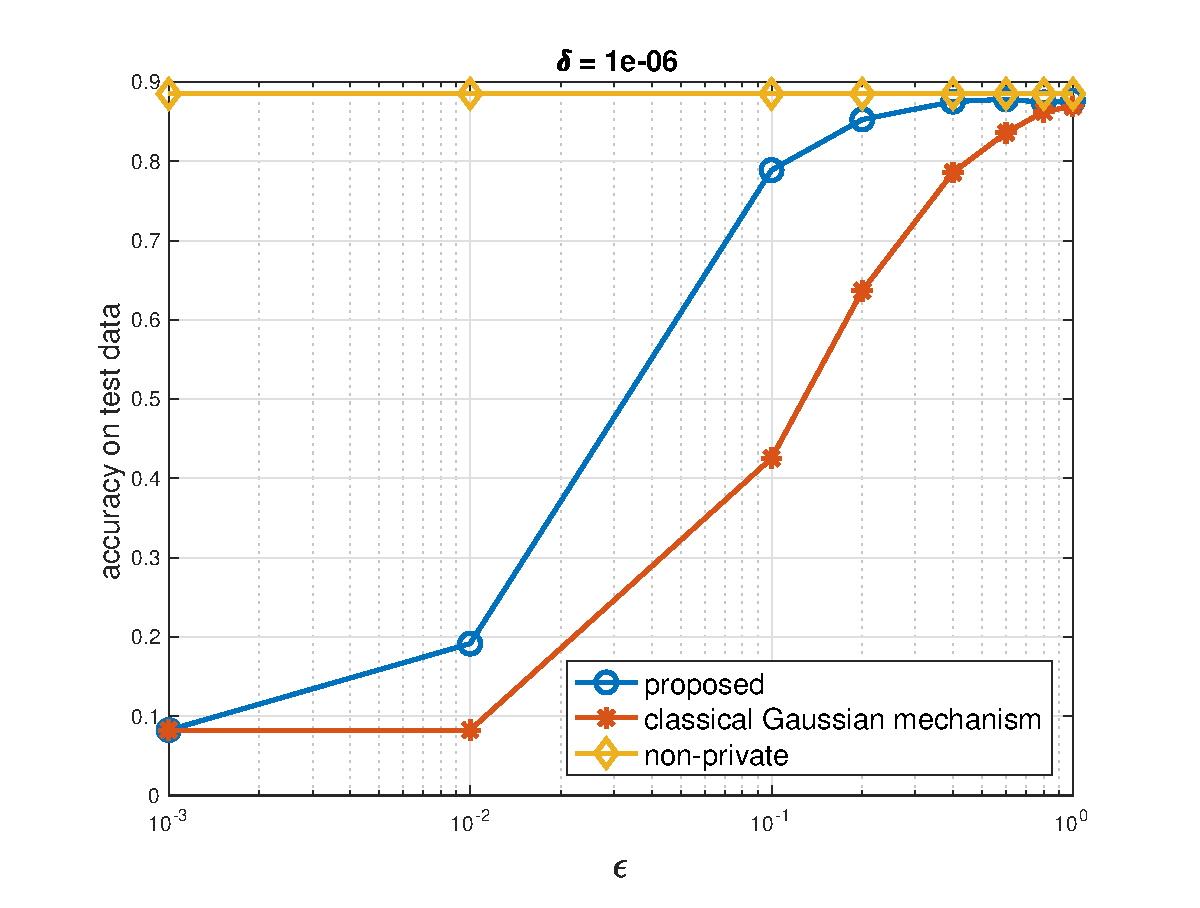
\includegraphics[width = 1.5in]{images/G_1}\label{fig_G_1}} \hfil \subfigure[$\delta = 1\mathrm{e}{-5}$.]{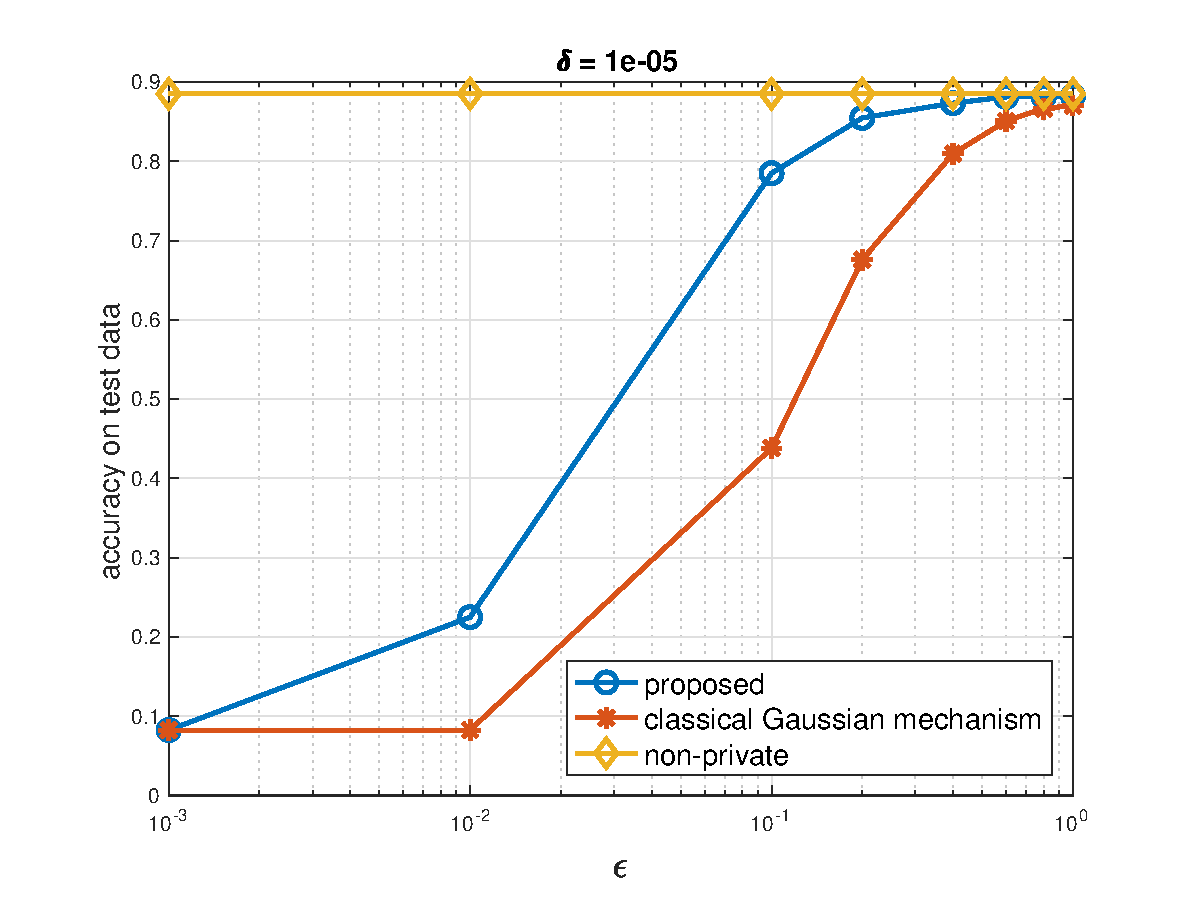
\includegraphics[width = 1.5in]{images/G_2}\label{fig_G_2}}}
\centerline{ \subfigure[$\delta = 1\mathrm{e}{-4}$.]{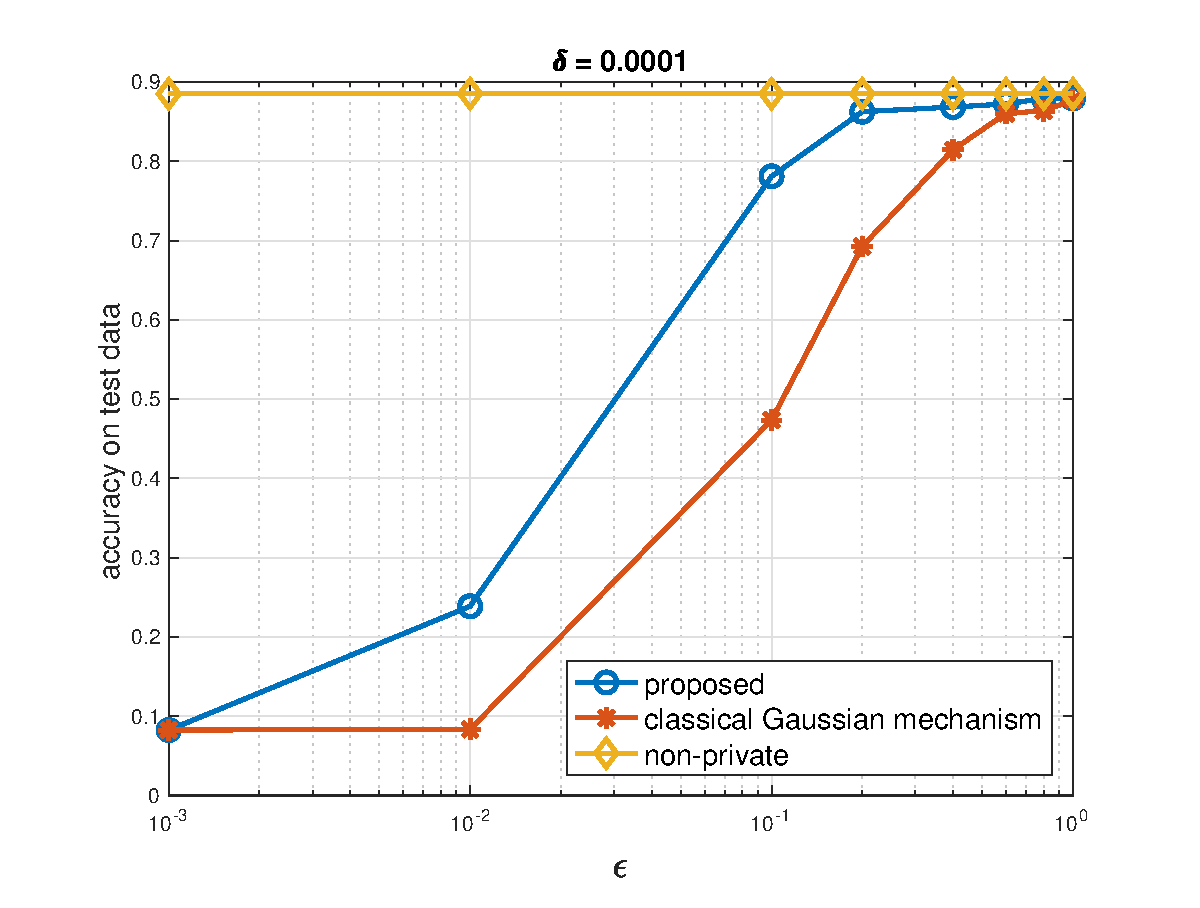
\includegraphics[width = 1.5in]{images/G_3}\label{fig_G_3}} \hfil \subfigure[$\delta = 1\mathrm{e}{-3}$.]{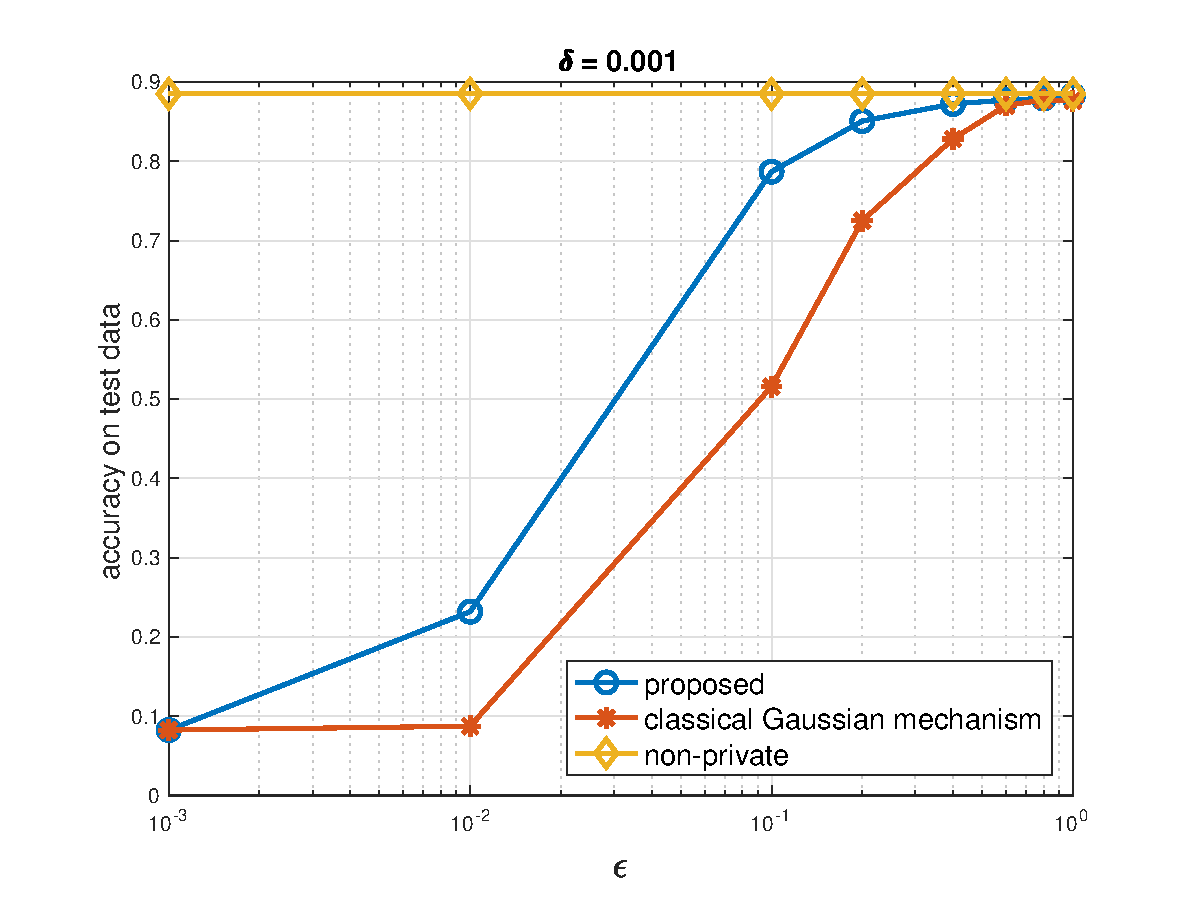
\includegraphics[width = 1.5in]{images/G_4}\label{fig_G_4}}}
\centerline{ \subfigure[$\delta = 1\mathrm{e}{-2}$.]{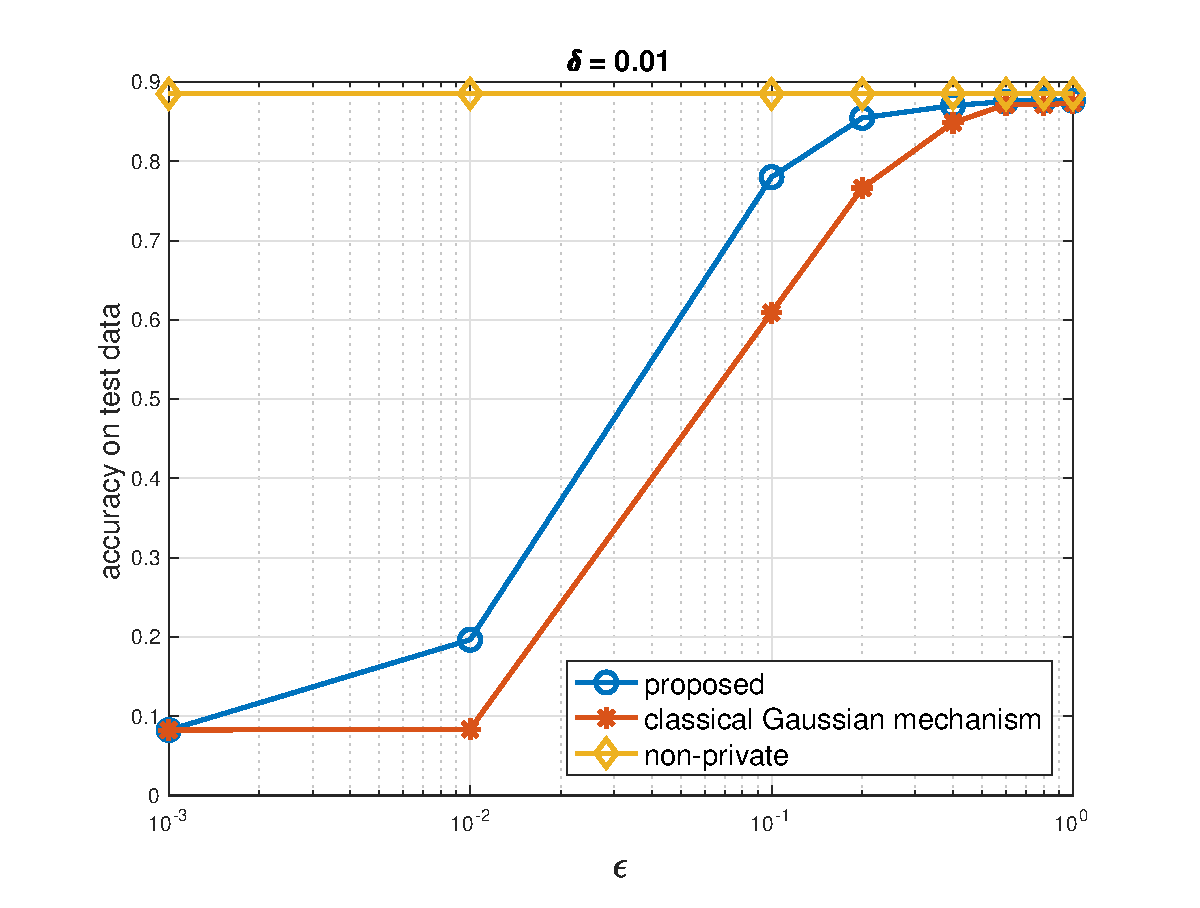
\includegraphics[width = 1.5in]{images/G_5}\label{fig_G_5}} \hfil \subfigure[$\delta = 1\mathrm{e}{-1}$.]{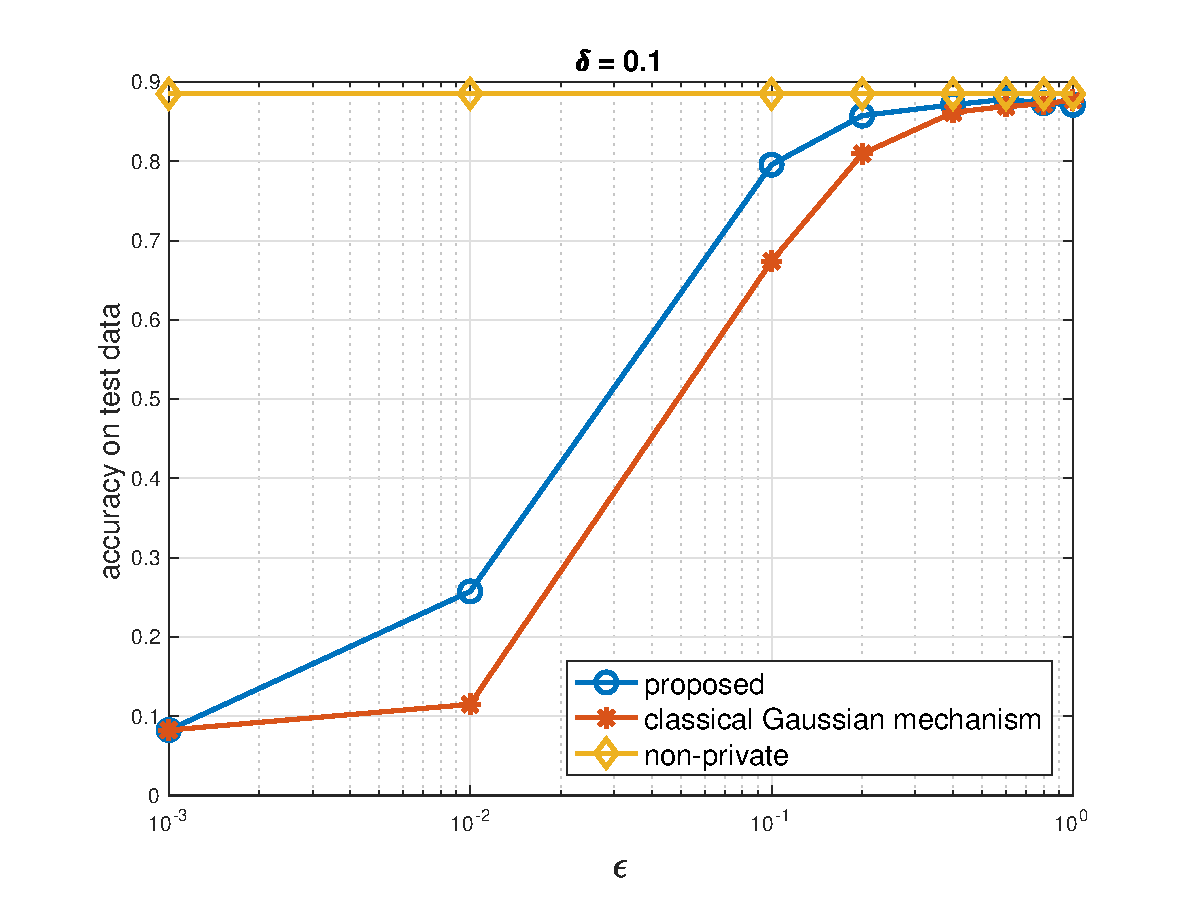
\includegraphics[width = 1.5in]{images/G_6}\label{fig_G_6}}}
\centerline{ \subfigure[$\delta = 0.5$.]{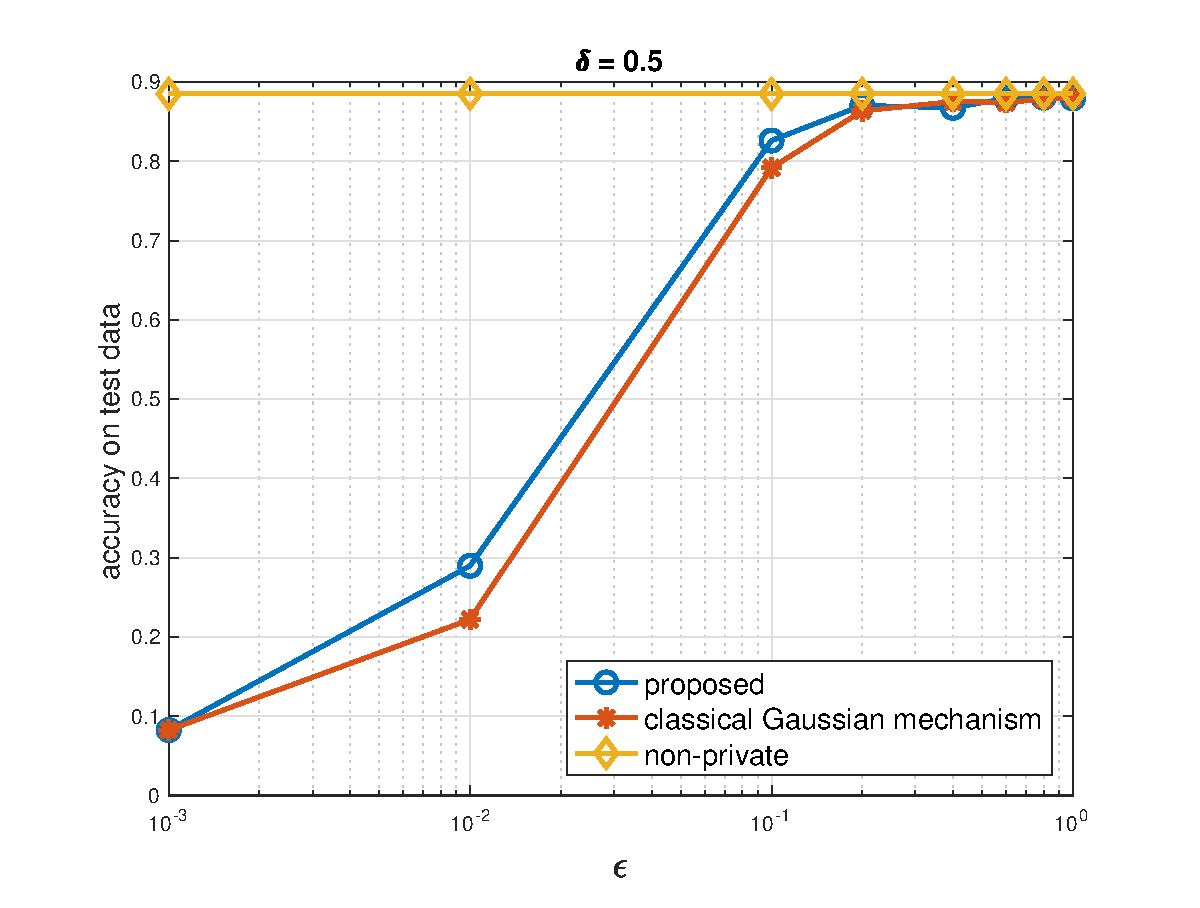
\includegraphics[width = 1.5in]{images/G_7}\label{fig_G_7}} \hfil \subfigure[$\delta = 0.9$.]{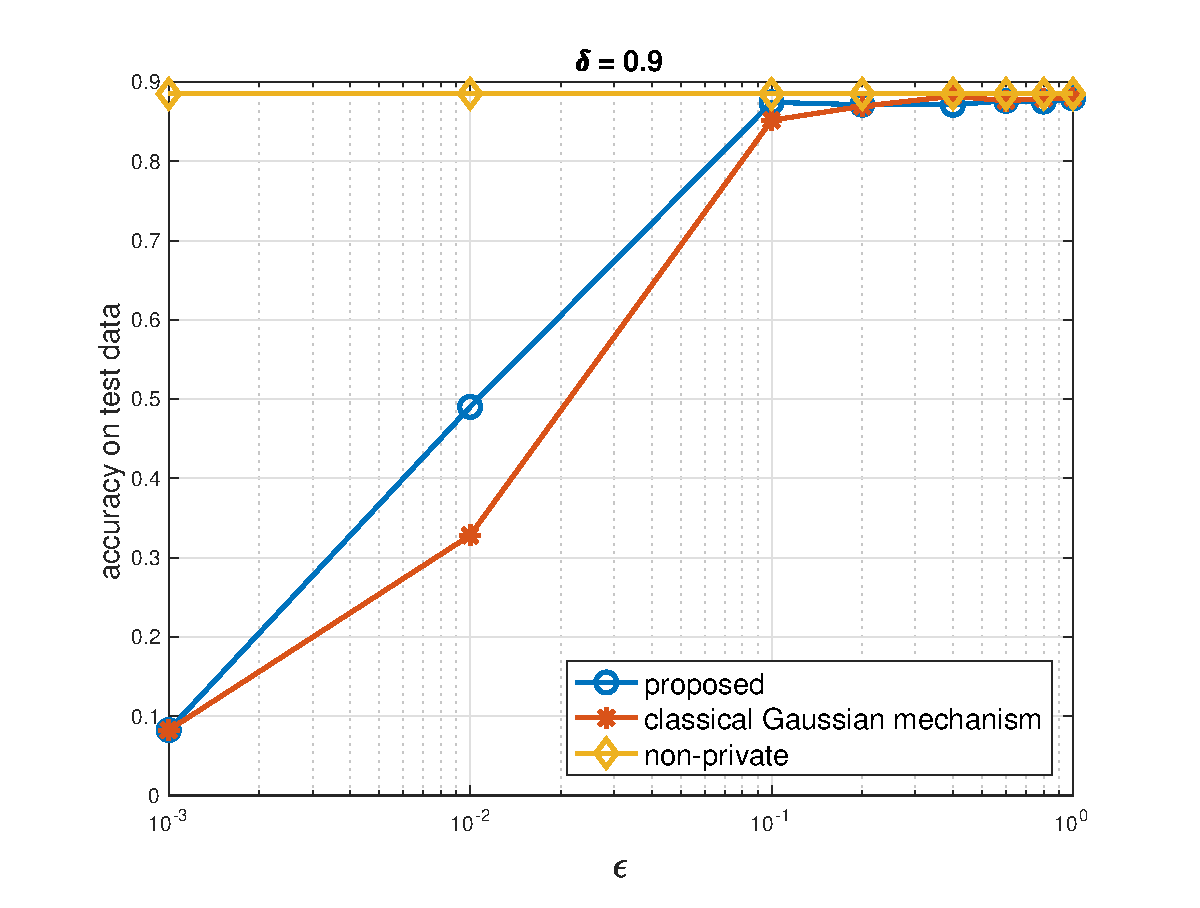
\includegraphics[width = 1.5in]{images/G_8}\label{fig_G_8}}}
\caption{The effect of $\epsilon$ on Freiburg test data classification accuracy.}\label{fig_G_first_part}
\end{figure}     
\begin{figure}
\centerline{ \subfigure[$\epsilon = 1\mathrm{e}{-3}$.]{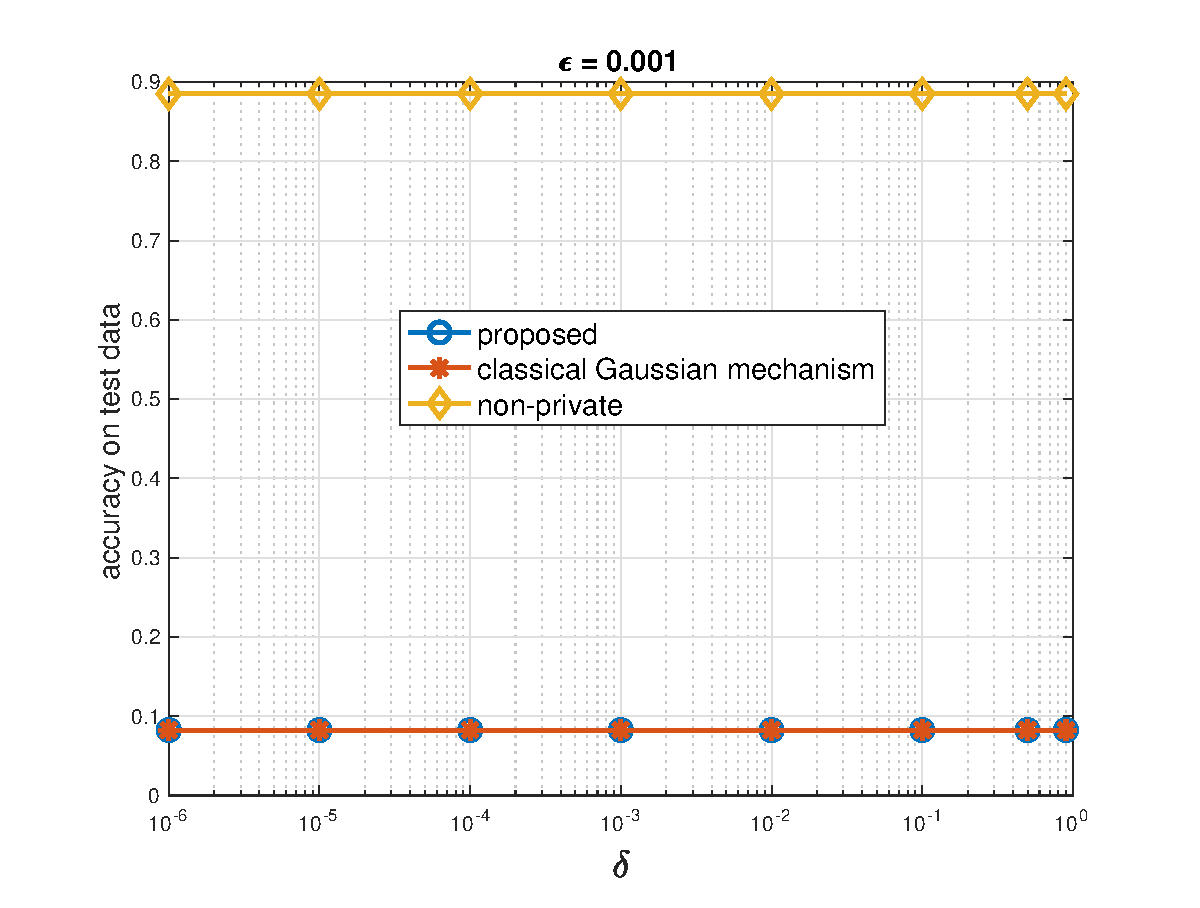
\includegraphics[width = 1.5in]{images/G_9}\label{fig_G_9}} \hfil \subfigure[$\epsilon = 1\mathrm{e}{-2}$.]{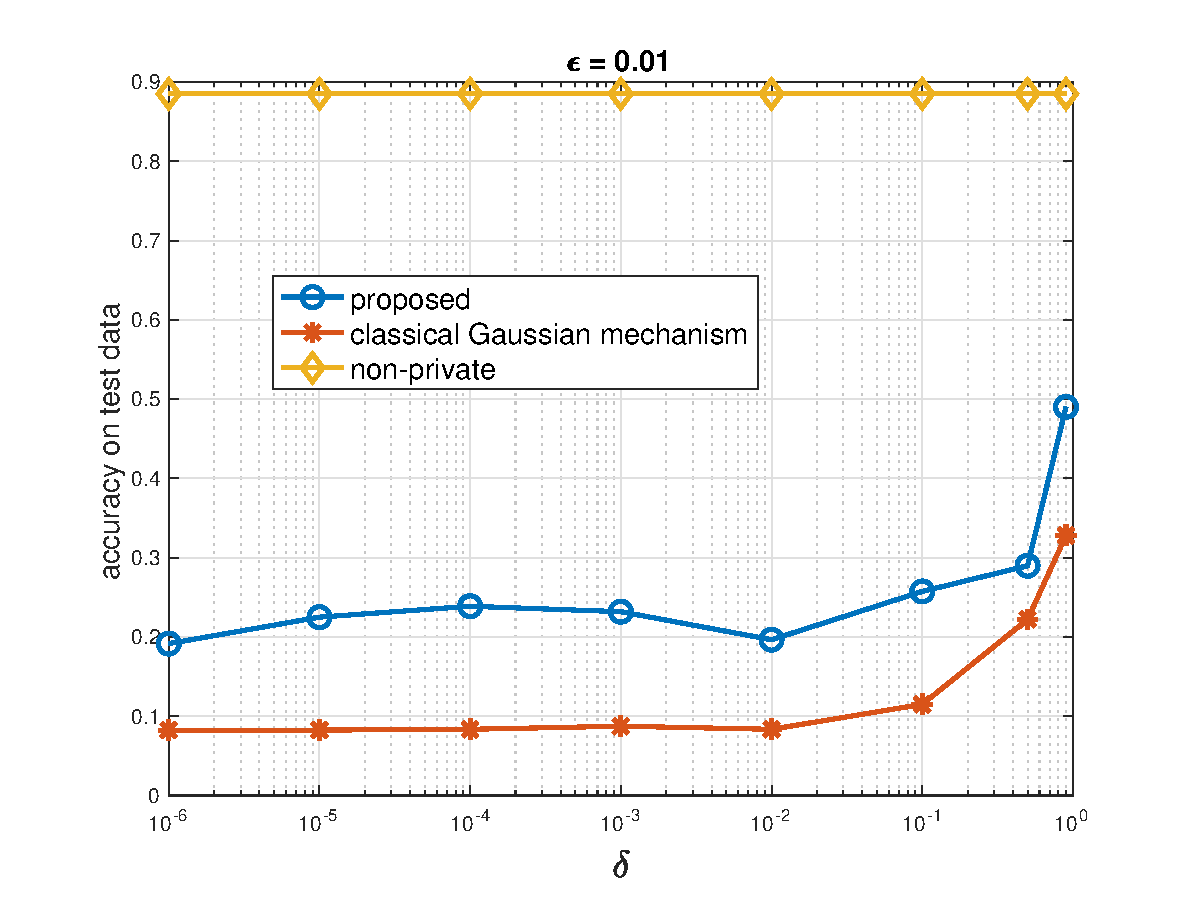
\includegraphics[width = 1.5in]{images/G_10}\label{fig_G_10}}}
\centerline{ \subfigure[$\epsilon = 1\mathrm{e}{-1}$.]{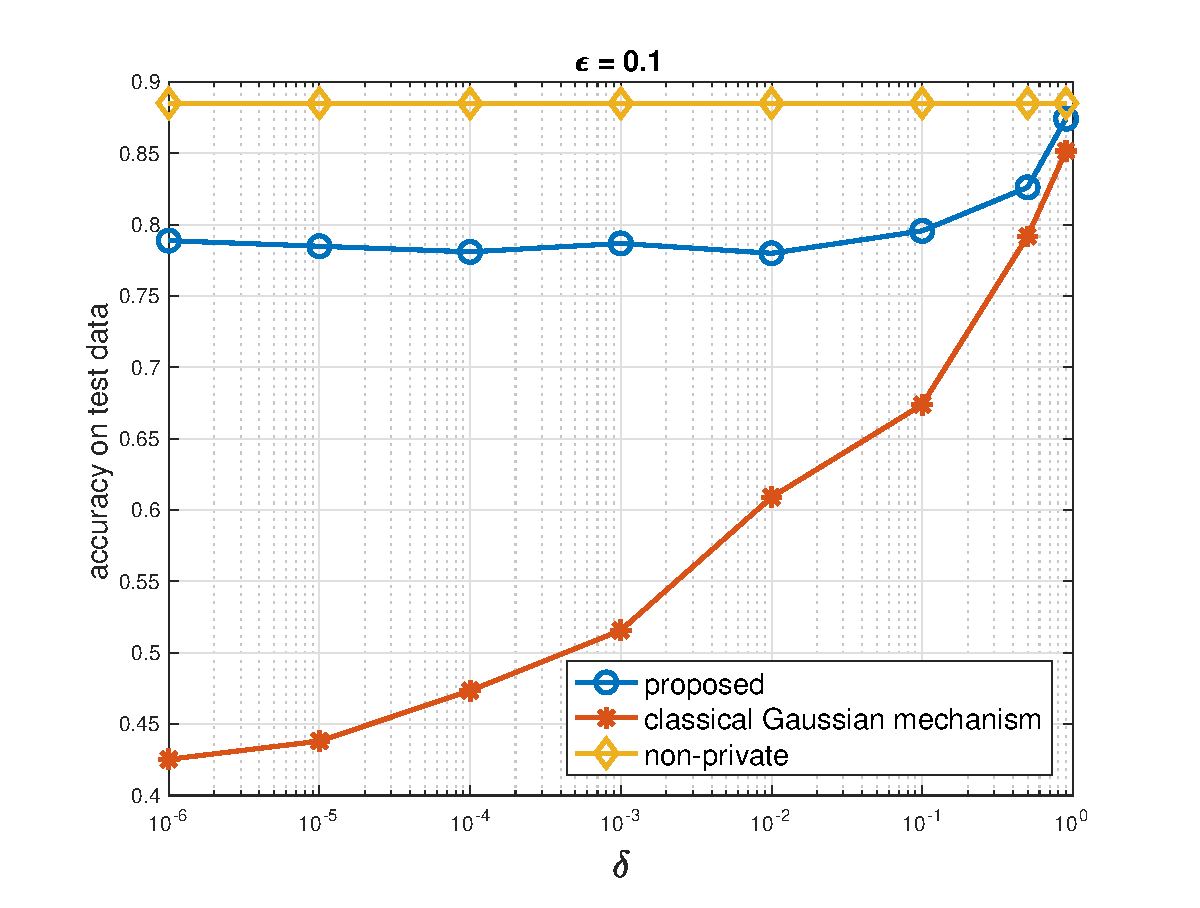
\includegraphics[width = 1.5in]{images/G_11}\label{fig_G_11}} \hfil \subfigure[$\epsilon = 0.2$.]{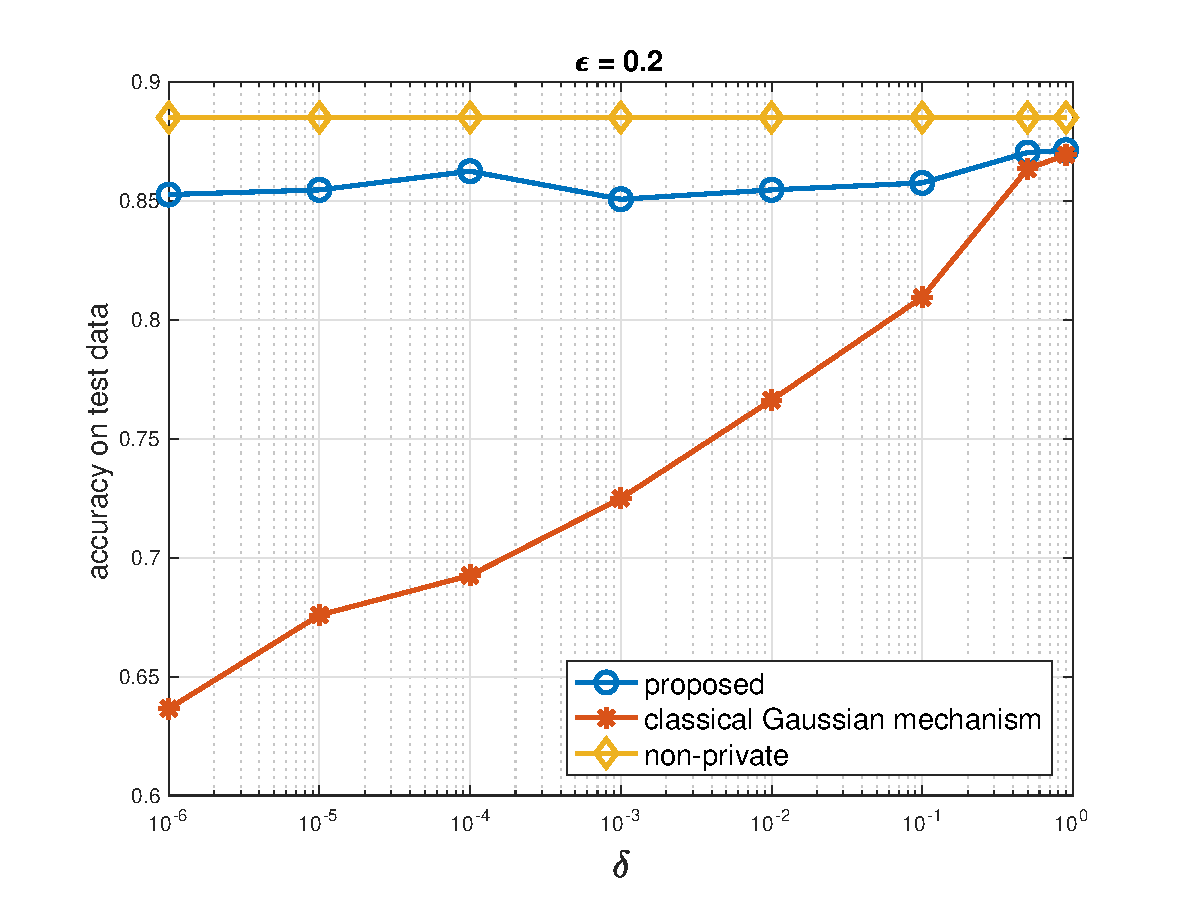
\includegraphics[width = 1.5in]{images/G_12}\label{fig_G_12}}}
\centerline{ \subfigure[$\epsilon = 0.4$.]{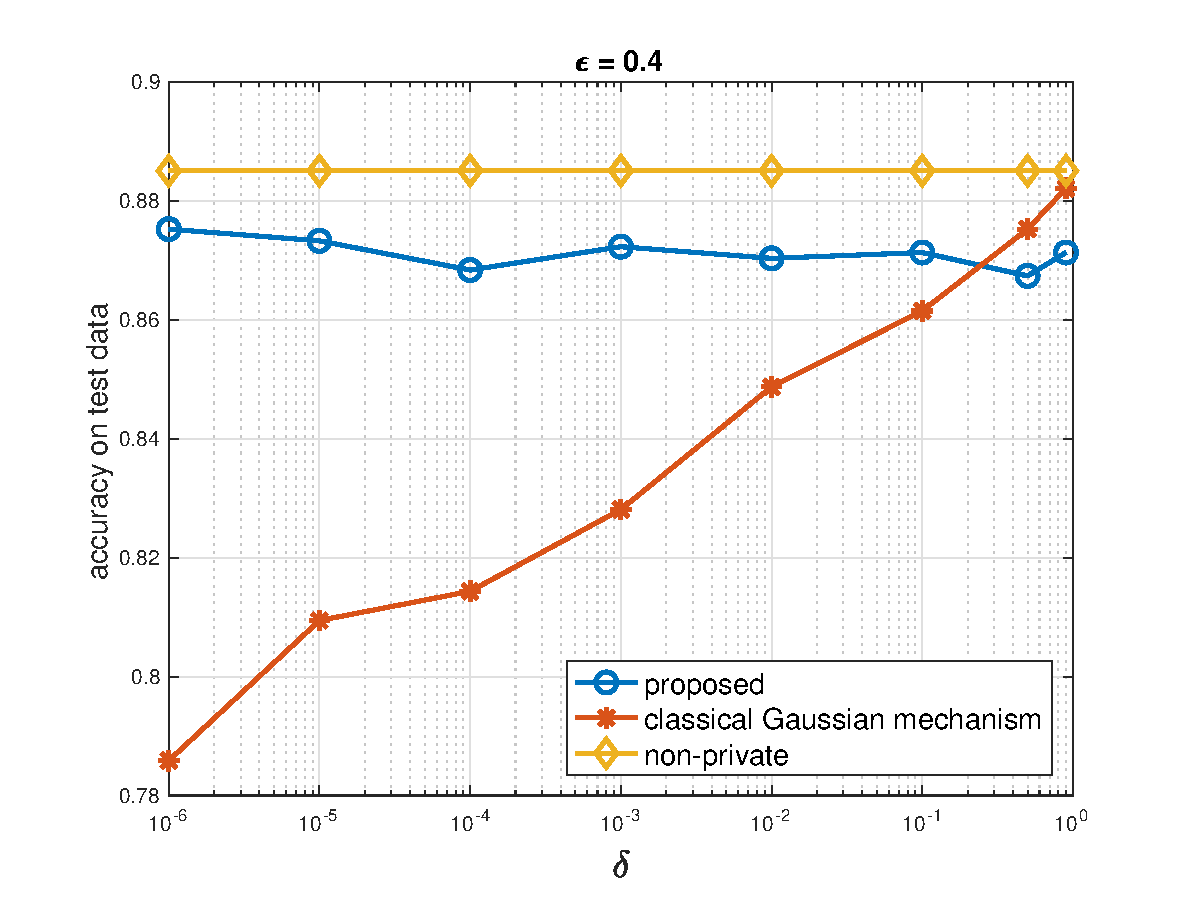
\includegraphics[width = 1.5in]{images/G_13}\label{fig_G_13}} \hfil \subfigure[$\epsilon = 0.6$.]{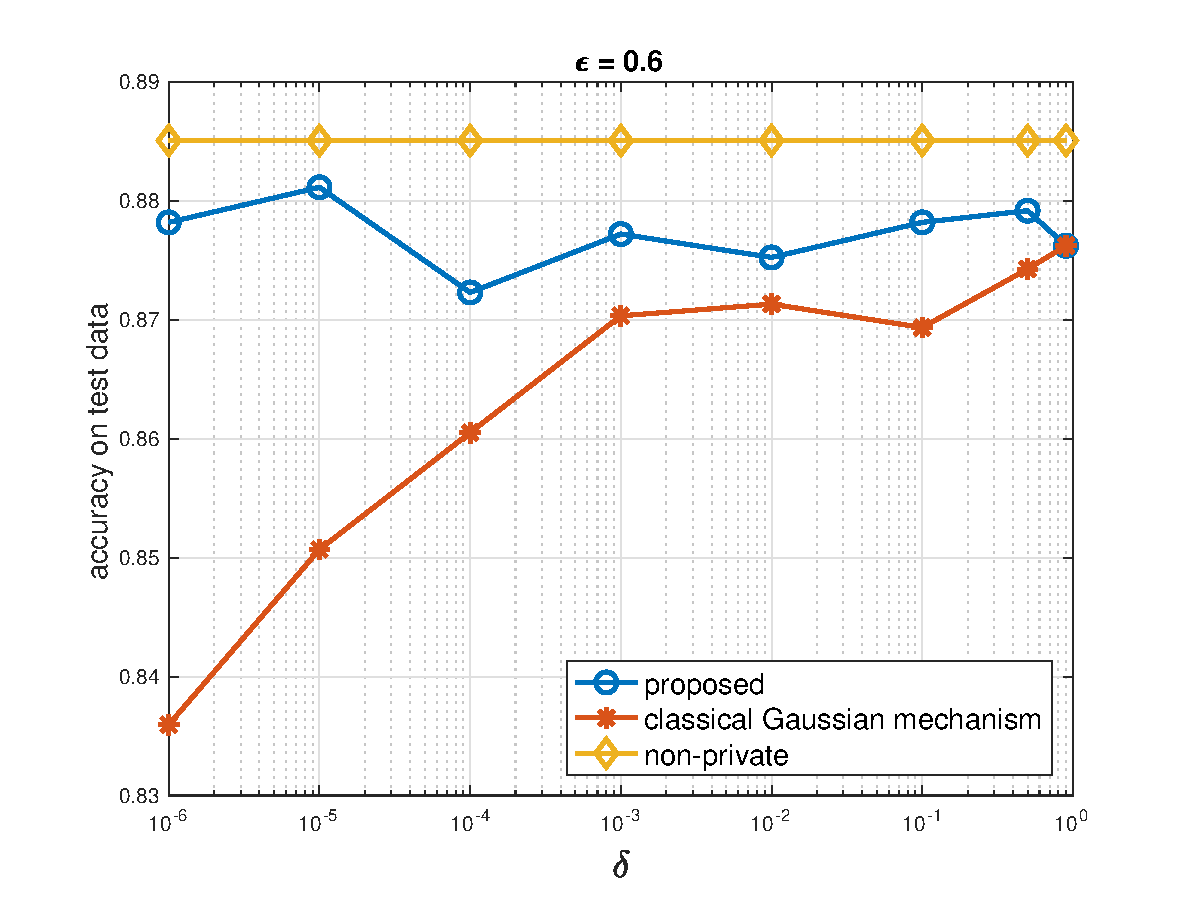
\includegraphics[width = 1.5in]{images/G_14}\label{fig_G_14}}}
\centerline{ \subfigure[$\epsilon = 0.8$.]{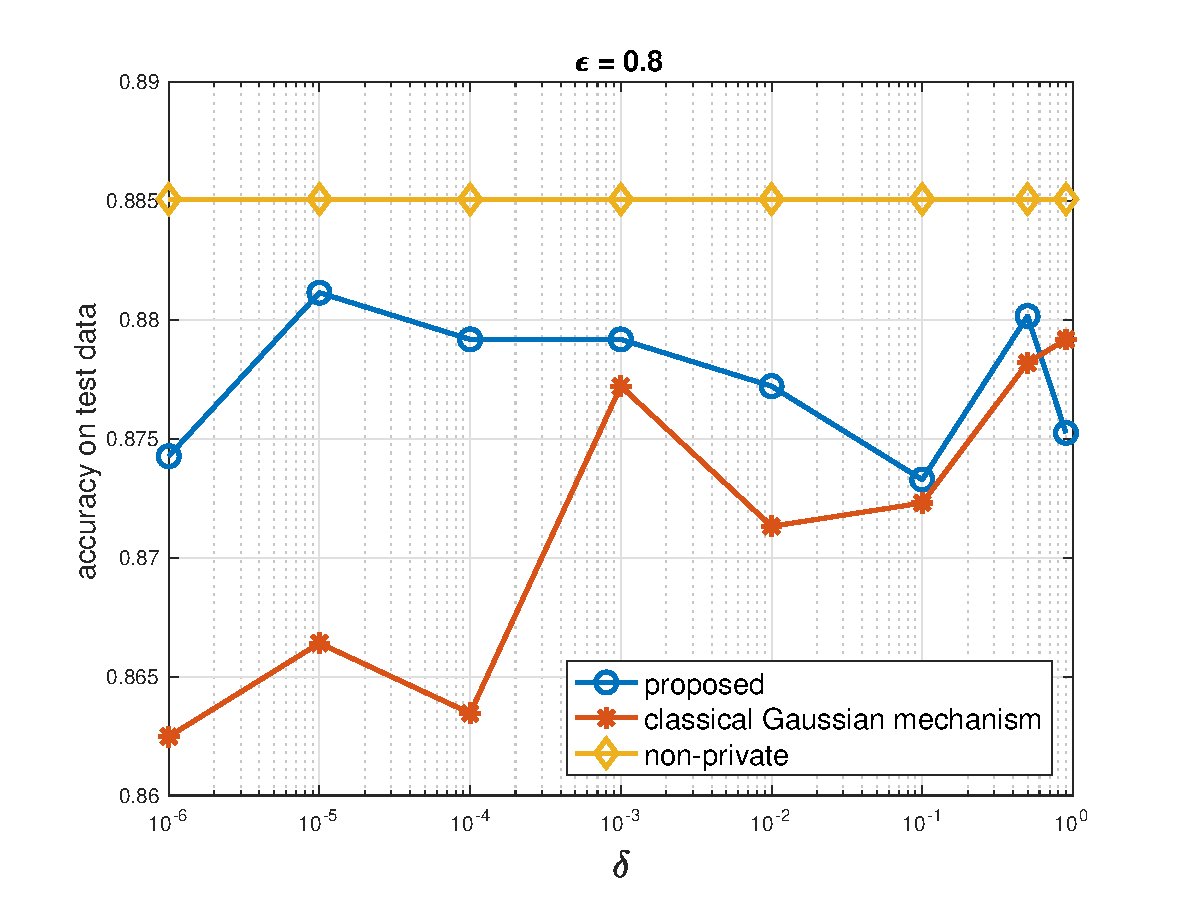
\includegraphics[width = 1.5in]{images/G_15}\label{fig_G_15}} \hfil \subfigure[$\epsilon = 1$.]{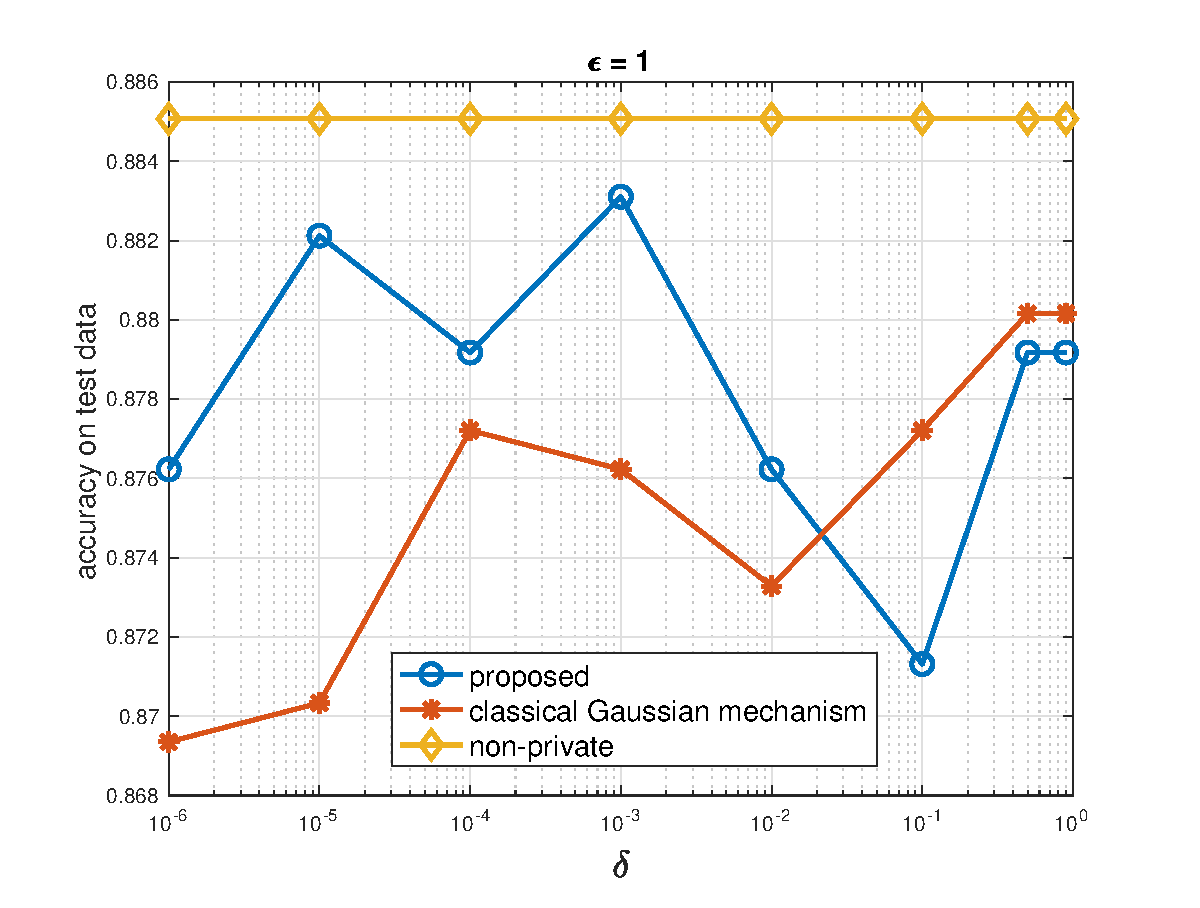
\includegraphics[width = 1.5in]{images/G_16}\label{fig_G_16}}}
\caption{The effect of $\delta$ on Freiburg test data classification accuracy.}\label{fig_G_second_part}
\end{figure} 
\subsubsection{Caltech-101 Dataset}
Catech-101~\cite{1384978} is a widely used dataset containing pictures of objects belonging to 101 categories. The dataset has 9144 images divided into 102 classes (101 object categories + one ``background'' category). Again, $8192-$dimensional feature vector is extracted from each image using AlexNet and VGG-16 followed by a normalization to have zero-mean and unity-variance along each dimension. As the classes have different number of images ranging from 31 to 800, we use a fixed number of training images per class and the classification performance is normalized across classes by calculating the average classification accuracy per class. The training set includes 30 randomly chosen images from each class and the rest images serve as the test images.
\begin{table}
\renewcommand{\arraystretch}{1.3}
\caption{Results of experiments on Caltech-101 dataset}
\label{table_results_caltech101} \centering
\begin{tabular}{c||c}
\hline
\bfseries method  & \bfseries $\begin{array}{c} \mbox{testing accuracy in \%} \\ \mbox{(averaged per class)} \end{array}$   \\
\hline \hline  
$(0.1,1\mathrm{e}{-6})-$differentially private proposed & \textbf{87.20} \\
$(0.1,1\mathrm{e}{-6})-$differentially private Gaussian & 36.92 \\
Non-private proposed & \textbf{88.05}   \\
Non-private SVM &    83.27      \\
Non-private Naive Bayes &  83.24    \\
Non-private Random Forest &  82.31    \\
Non-private $1$-NN & 79.16    \\
Non-private Decision Tree &  38.69  \\
\hline \hline
\end{tabular}
\end{table}        

The distributed learning scenario is created assuming that a class's complete training data is owned by a single participant. Thus, the number of participants is equal to 102. The method's $(\epsilon,\delta)-$differential privacy against perturbation (in one element of data vector), with perturbation magnitude upper bounded by $d = 0.1$, is studied. The experimental results have been summarized in Table~\ref{table_results_caltech101}. The results in Table~\ref{table_results_caltech101} further validate that    
1) The proposed optimal noise adding mechanism can result in multi-fold gain of the utility over the classical Gaussian mechanism. 2) The fuzzy based approach of this study offers a competitive alternative to the widely used machine learning methods for classification of high-dimensional data.

 
\subsubsection{Caltech-256 Dataset}
Caltech-256~\cite{griffinHolubPerona} is another challenging set of 30607 images labelled into 257 classes (256 object categories + one ``clutter'' category). A training set is built by choosing randomly 60 images from each of 257 classes and the rest images serve as testing set. The distributed learning scenario is created assuming that a class's complete training data is owned by a single participant. The method's $(\epsilon,\delta)-$differential privacy against perturbation (in one element of data vector), with perturbation magnitude upper bounded by $d = 0.1$, is studied. Table~\ref{table_results_caltech256}  reports the experimental results. The argument of competitive performance of proposed method is once again validated by the results stated in Table~\ref{table_results_caltech256}. 
\begin{table}
\renewcommand{\arraystretch}{1.3}
\caption{Results of experiments on Caltech-256 dataset}
\label{table_results_caltech256} \centering
\begin{tabular}{c||c}
\hline
\bfseries method  & \bfseries $\begin{array}{c} \mbox{testing accuracy in \%} \\ \mbox{(averaged per class)} \end{array}$   \\
\hline \hline  
$(0.1,1\mathrm{e}{-6})-$differentially private proposed & \textbf{74.54} \\
$(0.1,1\mathrm{e}{-6})-$differentially private Gaussian & 29 \\
Non-private proposed & \textbf{77.25}   \\
Non-private SVM &    69.24      \\
Non-private Naive Bayes &  65.22    \\
Non-private Random Forest &  63.66    \\
Non-private $1$-NN & 61.64    \\
\hline \hline
\end{tabular}
\end{table}    






\textbf{USTAN to provide the use case description and evaluation framework. Everyone to contribute once we have a clear idea about how to do evaluation}

%Need 2 to 3 pages on how we test serums?

{\color{purple}
Some thoughts/comments here:
\begin{itemize}
    \item Some evaluations will be from experts and some kinds of users (or through the use cases directly). These include areas like correctly being able to use the system, being able to authenticate well, etc.
    \item Some evaluations are ``formal'' in the sense that the goal is to use (semi-)formal methods to prove correctness. This includes the differential privacy, verification of components, modelling the system and showing results on the model, etc.
    \item We could consider compliance to be an evaluation criteria, e.g.~do we actually meet GDPR requirements.
    \item We may wish to link some of the above (or other) evaluation approaches to the KPIs we plan to have for the project.
    \item It may be helpful to link these to the earlier parts of the paper when done; e.g.~data fabrication is tested using technique X and shown that the fabricated and real data are indistinguishable.
\end{itemize}}




Zuyderland Medisch Centrum, Netherlands

%Need basic use case with picture

\begin{figure}[ht!]
    \centering
    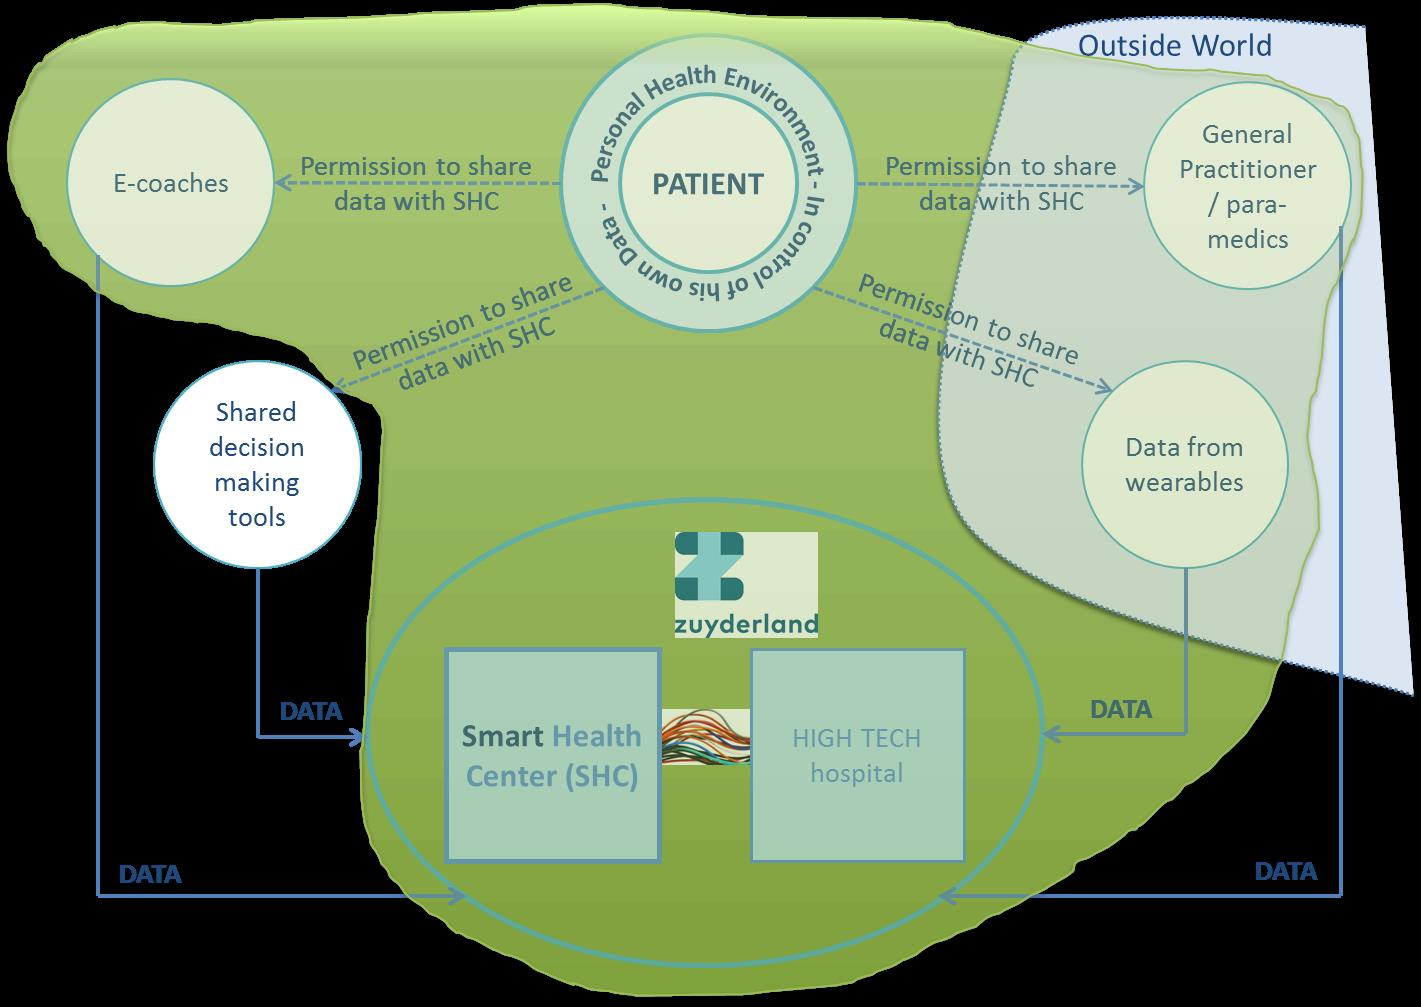
\includegraphics[width=70mm]{images/UseCaseZuyderland.jpg}
    \caption{Use Case Zuyderland}
    \label{fig:usecasezuyderland}
\end{figure}

Fundacio Clinic per a la Recerca Biomedica, Spain

\url{http://web.fundacioclinic.org/Home/tabid/499/language/en-US/Default.asx}

% Need 2-3 pages

% AV - Requested a copy of this case study - 201906-26

Joana's Journey through the Fundacio Clinic's services.

\begin{figure}
    \centering
    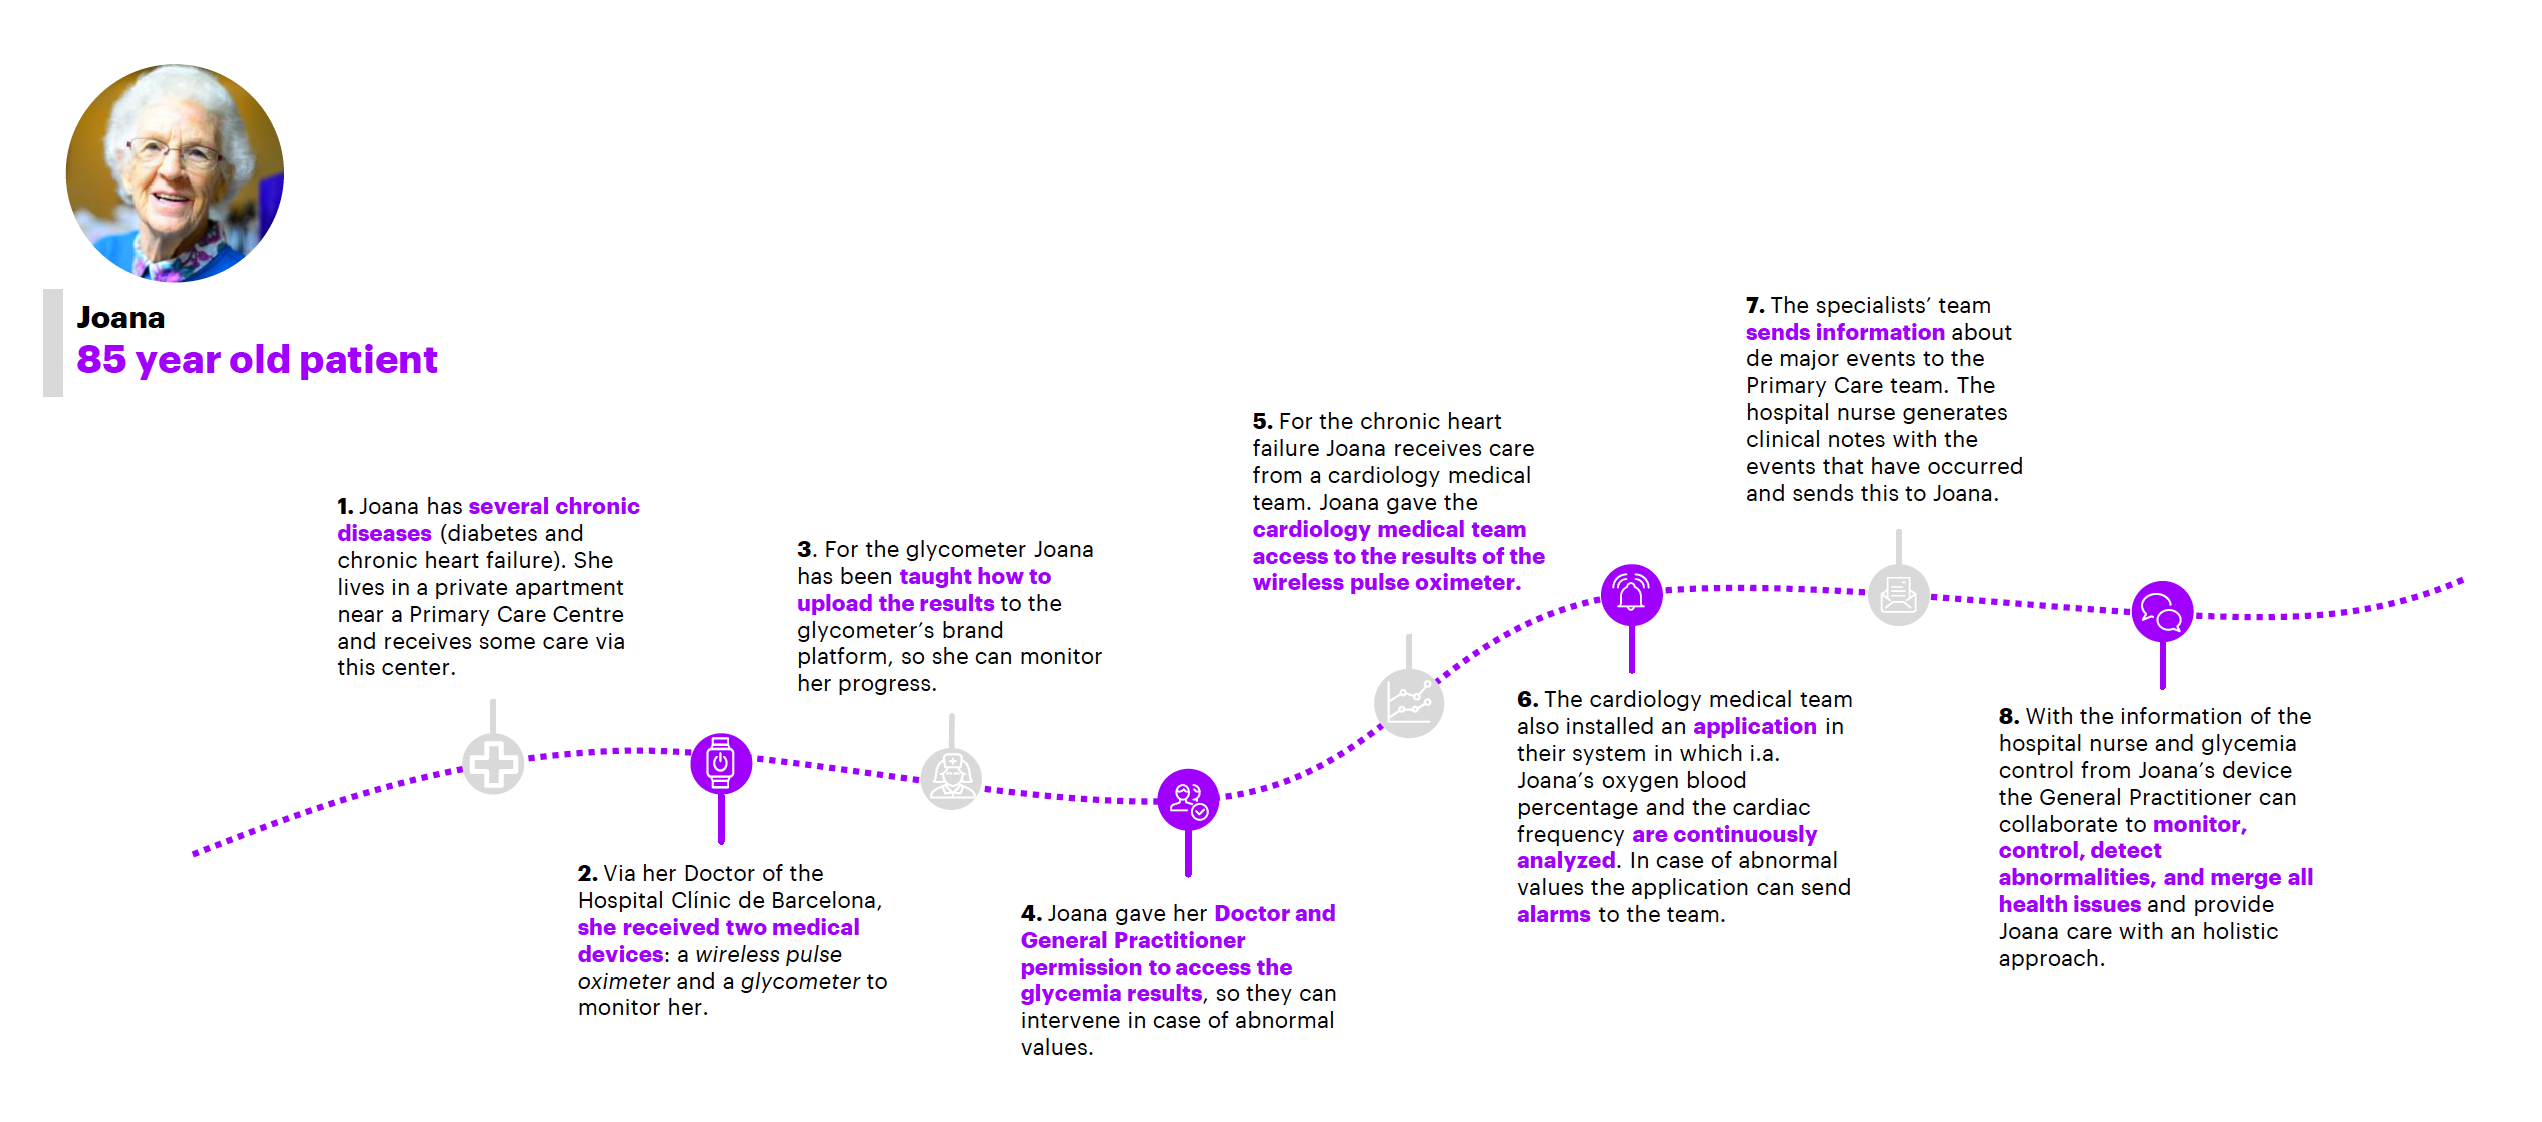
\includegraphics[width=75mm]{images/FCRB-Use-Case.png}
    \caption{Joana's Journey}
    \label{fig:usecasefcrb}
\end{figure}


\subsection{Use Case - Edinburgh Cancer Gateway}

\noindent
In the use case that we consider, we developed a dashboard to help the oncologist observe, monitor, and analyse the patients' condition as well as the chemotherapy treatments which might improve the well-being and survival rate of the patients. Our ultimate aim is to build a \emph{toxicity predictors model} (Figure~\ref{fig:USTANDiagram} to predict toxicity of the treatment based on treatment history and feedback from patients.

\begin{figure}[t!]
    \centering
    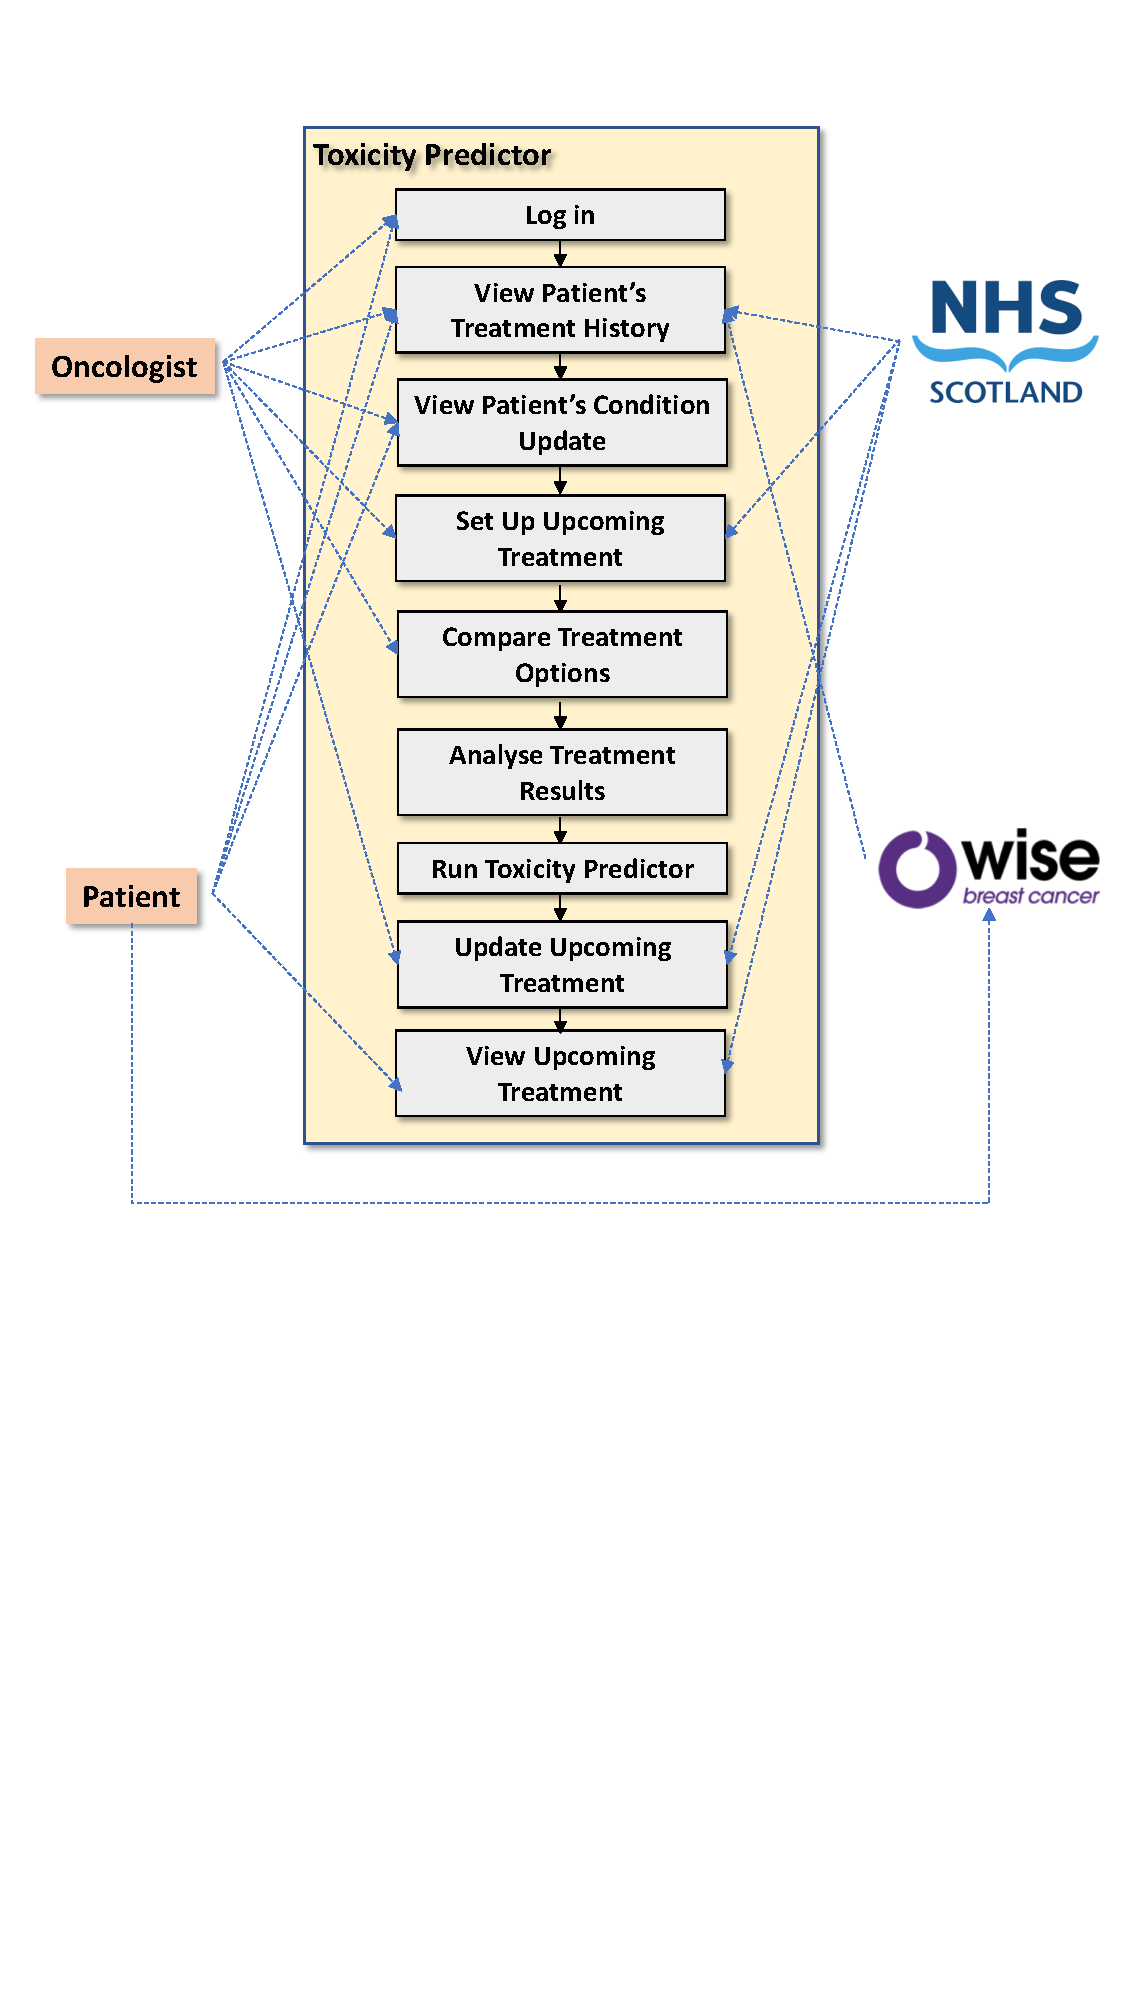
\includegraphics[width=0.45\textwidth]{images/USTANUseCaseDiagram.pdf}
    \caption{Toxicity Predictor for Breast Cancer Treatment}
    \label{fig:USTANDiagram}
\end{figure}

\begin{figure}[t!]
    \centering
    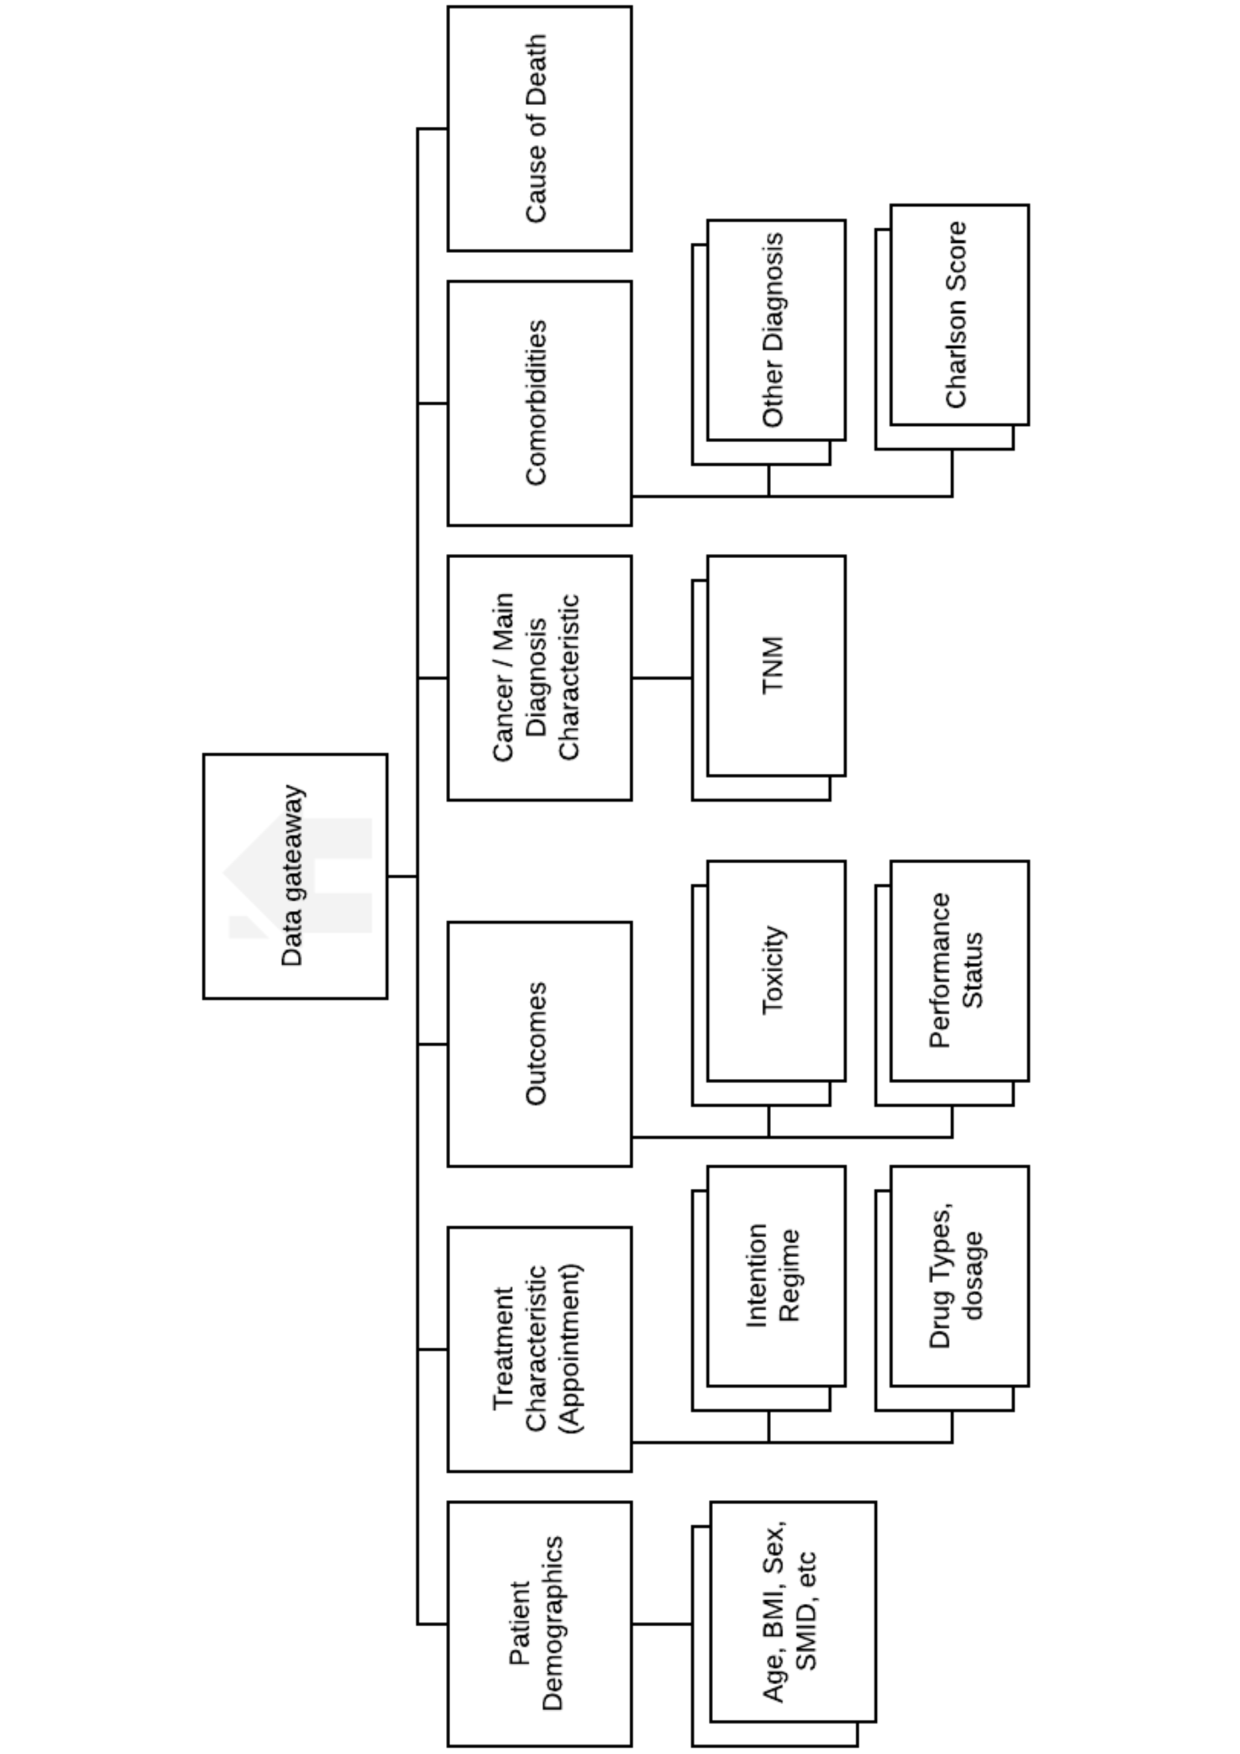
\includegraphics[angle=-90,width=0.45\textwidth]{images/ECG.pdf}
    \caption{Database Structure for Training the Toxicity Predictor Model}
    \label{fig:ECG}
\end{figure}
Figure~\ref{fig:ECG} shows the data structure we use for training the toxicity predictors model. We extracted the data during the initial step for training the machine learning models from three main databases (i.e., Chemocare, Trak, and Oncology DB) in the Edinburgh Cancer Centre (ECC). The data contains the information on treatment cycles, recorded side effects (here, toxicity level), comorbidities, and various observations concerning breast cancer patients for three years (from 2014 to 2016). The extraction has data for 51661 treatments, of which 13030 are of breast cancer treatments. There are 933 unique patients, and some patients may have two or three different treatments/regimes. Each regime has several cycles ranging from one to more than 50 cycles (e.g., 85) [cite: On Predicting the Outcomes of Chemotherapy Treatments in Breast Cancer].

\subsection{Evaluation Framework}

\subsection{Smart Patient Records}

\subsection{Data Fabrication}

\subsection{Blockchain}

\subsection{Authentication}

\subsection{Data Analytics}

%Need 2-3 pages on use case.


\section{Related Work}
Chen et al. in~\cite{deepChain} present DeepChain, a framework that combines the distributed deep learning with blockchain technology to achieve XX. 

Wang et al. in~\cite{healthdataQuery} describe a method to optimise the queries on medical data. 

Unified Medical Language System (UMLS~\cite{UMLS}) represents an attempt to integrate and distribute key terminology, classification and coding standards, and associated resources to promote creation of more effective and interoperable biomedical information systems and services, including electronic health records.

OpenEHR Specification Program~\cite{OpenEHR} provides specifications and their computable expressions to enable development and deployment of open, interoperable and computable patient-centric health information systems.

Shade~\cite{shade} is a framework for Apache Spark, a cluster computing framework, that provides strong privacy guarantees for users even in the presence of an informed adversary, while still providing high utility for analysts. It includes two mechanisms - SparkLAP, which provides Laplacian perturbation based on a user's query and SparkSAM, which uses the contents of the database itself in order to calculate the perturbation.

Palanisami et al.~\cite{privacyAware} present a privacy-aware data disclosure scheme that considers group privacy requirements of individuals in bipartite association graph datasets where even aggregate information about groups of individuals may be sensitive and need protection.

\textbf{Everyone to contribute}

\section{Conclusion}

\noindent
%The health centers of the future will be highly distributed and, due to convenience and cost effectiveness, will need to integrate home-, work- and environment-based monitoring with centralised hospital diagnostics and treatment services. 
In this paper, we have outlined the problems that the distributed health systems of the future will face in terms of safe storing and sharing of confidential patient data. %, especially taking into account more and more strict regulations and legislations (such as GDPR) that govern the ownership and access rights to personal data. 
We have also proposed the \emph{SERUMS} methodology for managing confidential, distributed medical data, covering all the phases in its lifetime, from retrieval and storing to end-point data analytics. Furthermore, we have described the initial versions of the tools from the \emph{SERUMS} tool-chain, including new universal smart patient record format, blockchain for controlling access to the health records and recording lineage of the data, authentication mechanisms for logging in to healthcare systems and privacy-preserving data analytics techniques. We have also described Data Fabrication Platform (DFP), a platform for generating large volumes of synthetic but realistic medical data that will be used for development and evaluation of the \emph{SERUMS} tool-chain. Finally, we have described its proposed use in the \emph{Edinburgh Cancer Gateway} use case that collects and analyses information about effects of chemotherapy treatments on breast cancer patients, to predict the outcome of the treatment and improve treatment.
%
%In future, we plan to develop the final versions of the tools in the \emph{SERUMS} tool-chain, investigate interoperability issues between them and integrate them into the \emph{SERUMS} methodology. We also plan to evaluate the tool-chain on two further large-scale use cases - a system for a new hospital that will be built by Zuyderland Medisch Centrum, one of the \emph{SERUMS} project partners, and a system for Fundacio Clinic per a Reserca Biomedica in Barcelona.


\section*{Acknowledgment}

The authors would like to thank...
more thanks here



\begin{thebibliography}{1}

\bibitem{IEEEhowto:kopka}
H.~Kopka and P.~W. Daly, \emph{A Guide to \LaTeX}, 3rd~ed.\hskip 1em plus
  0.5em minus 0.4em\relax Harlow, England: Addison-Wesley, 1999.
  
 \end{thebibliography}

\end{document}